%% inicio, la clase del documento es iccmemoria.cls
\documentclass{iccmemoria}
\usepackage[onelanguage, commentsnumbered, linesnumbered, boxed, ruled]{algorithm2e}
\usepackage{pdfpages}
\usepackage{amsfonts}
\usepackage{amssymb}
\usepackage{array}
\usepackage{longtable}
\usepackage{float}
\usepackage{especificacionutility}

%% datos generales y para la tapa
\titulo{Herramienta para la optimizaci�n de redes de distribuci�n de agua potable}
\author{Gabriel Gonzalo Alexander Sanhueza Fuentes}
\supervisor{Jimmy Gutierrez Bahamondes}
\cosupervisor{Daniel Mora Melia}
\informantes
	{Profesor Informante 1}
	{Profesor Informante 2}
\adicional{(s�lo por si se necesita agregar alg�n otro profesor)}
\director{Profesor del ramo Memoria de T�tulo}
\date{mes, a�o}

%% inicio de documento
\begin{document}

%% crea la tapa
\maketitle

%% dedicatoria
\begin{dedicatory}
Dedicado a ...
\end{dedicatory}

%% agradecimientos
\begin{acknowledgment}
Agradecimientos a ...
\end{acknowledgment}

%% indices
\tableofcontents
\listoffigures
\listoftables

%% resumen
\input{Resumen/Resumen}

%% abstract

\chapter{Introducci�n}
El proyecto que se desarrollara consiste en la creaci�n de una herramienta que haga uso de algoritmos metaheur�sticos para tratar y minimizar problemas existentes en redes de distribuci�n de agua potable.

Este proyecto solo abarcara dos problemas existentes dentro de las redes de distribuci�n de agua potable.

Para el desarrollo de este proyecto se usar�n librer�as ya existentes con el fin de reducir el tiempo de desarrollo. Estas librer�as son epanet2.dll, desarrollada en c, y JNA, librer�a en java para funciones nativas.


\section{Prop�sito del sistema}

El proyecto consiste en el desarrollo de un sistema que permita simular y buscar soluciones a problemas presentes en las redes de distribuci�n de agua potable haciendo uso de algoritmos metaheur�sticos. Adem�s, este sistema ser� desarrollado de tal forma que sea escalable con el fin de que otros desarrolles o investigadores sean capaces de extender su funcionalidad f�cilmente agregando nuevos algoritmos metaheur�sticos y problemas a tratar en el contexto de la distribuci�n de redes de agua potable.

\section{Alcance del proyecto}

Al final del periodo de desarrollo la herramienta contara con las siguientes prestaciones.
\begin{itemize}
    \item El sistema permitir� la carga y la visualizaci�n de la red gr�ficamente.
    \item El sistema inicialmente solo resolver� dos clases de problemas de optimizaci�n, uno monoobjetivo y el otro multiobjetivo. El problema monoobjetivo ser� el de los costos de inversi�n. En cuanto al problema multiobjetivo, este ser� el de los costos energ�ticos y el n�mero de encendidos y apagado de las bombas.  
    \item El sistema inicialmente �nicamente contara con dos algoritmos implementados los cuales ser�n el algoritmo gen�tico y NSGAII. El algoritmo gen�tico ser� el usado para tratar el problema monoobjetivo, mientras que NSGAII ser� aplicado al multiobjetivo.
\end{itemize}

Este proyecto no contempla la creaci�n de la red por lo que estas deber�n ser ingresadas como entradas al programa. La creaci�n de las redes puede realizarse a trav�s de EPANET. Adem�s, esta herramienta �nicamente podr� ser ocupada en equipos cuyo sistema operativo sea Windows debido a que se realizan llamadas a librer�as nativas.

\section{Contexto del proyecto} 
La escasez de agua potable es sin duda una problem�tica a nivel mundial y la optimizaci�n de los sistemas que permiten su distribuci�n es cada d�a m�s relevante. Existe una serie de problem�ticas asociadas a la determinaci�n de las condiciones �ptimas de operaciones y las caracter�sticas adecuadas para su construcci�n.

Las RDA son redes que pueden ser muy extensas y complejas. Forman parte de la estructura principal de cualquier ciudad. Deben ser capaces de adaptarse a los cambios y asegurar niveles m�nimos de servicios durante las 24 horas del d�a~\cite{Pereyra2017}. Adicionalmente, dependiendo de su topolog�a, las RDA integran sistemas de bombeo que requieren gran cantidad de energ�a en horarios determinados.

La optimizaci�n de estos sistemas, a la vez, involucra la participaci�n de m�ltiples criterios que deben ser tomados en cuenta a la hora de decidir. Sin embargo, la incorporaci�n de �stos, involucra la generaci�n de modelos cada vez m�s complejos~\cite{JHawanet-2019}.

Por lo anteriormente mencionado, esta �rea, ha llamado la atenci�n de muchos investigadores que han creado diversos m�todos para resolver la problem�tica desde diferentes enfoques. Sin embargo, a�n existen muy pocas aplicaciones computacionales que permitan emplear los nuevos modelos y t�cnicas de forma pr�ctica. �sto supone un gran problema para los interesados en aplicar estos conocimientos en un contexto real. Generalmente se trata de personas instruidas en tem�ticas relacionadas con la hidr�ulica pero que poseen un escaso manejo de t�cnicas computacionales de optimizaci�n.

En este trabajo se pretende dar respuesta a esa necesidad creciente a trav�s del dise�o e implementaci�n de una aplicaci�n de escritorio. Este nuevo sistema, permitir� a a los usuarios resolver dos de los principales problemas en la optimizaci�n de RDA. En el caso de los problemas con solo un objetivo se utilizar� un algoritmo gen�tico, mientras que en los problemas multiobjetivos se utilizar� NSGAII.
\section{Definiciones, siglas y abreviaturas}

\begin{description}
    \item [\textit{Genetic Algorithm (GA)}:] Estrategia de b�squeda de soluciones basada en la teor�a de la evoluci�n de Darwin. Para realizar esto, el algoritmo  parte desde un conjunto de soluciones denominada poblaci�n he iterativamente, lleva a cabo un proceso de reproducci�n, generando nuevas soluciones~\cite{Heiss-Czedik1997}.
    \item [\textit{Non-dominated Sorting Genetic Algorithm (NSGAII)}:] Algoritmo que utiliza el cruzamiento, mutaci�n y reproducci�n para encontrar un conjunto de soluciones optimas a problemas que cuentan con m�s de un objetivo~\cite{Deb2002}.
    \item [\textit{Metaheuristicas}:] Algoritmos que permiten resolver un amplio rango de problemas de optimizaci�n empleando t�cnicas con alg�n grado de aleatoriedad para encontrar soluciones a un problema. Estos algoritmos no garantizan que la soluci�n encontrada sea la �ptima, pero permiten obtener generalmente aproximaciones a esta~\cite{Yang2015, Boussaid2013, Luke2013}.
    \item [\textit{Java Reflection}:] Caracter�stica de java que permite que un programa se auto examine. Esta caracter�stica est� disponible a trav�s de la \textit{Java Reflection API}, la cual cuenta con m�todos para obtener los \textit{meta-object} de las clases, m�todos, constructores, campos o par�metros. Esta API tambi�n permite crear nuevos objetos cuyo tipo era desconocido al momento de compilar el programa~\cite{Braux1999}.
    \item [\textit{Java Annotation}:] Caracter�stica de java para agregar metadatos a elementos de java (clases, m�todos, par�metros, etc.)~\cite{Rocha2011}. Las anotaciones no tienen efecto directo sobre el c�digo, pero cuando son usadas junto con otras herramientas pueden llegar a ser muy �tiles. Estas herramientas pueden analizar estas anotaciones y realizar acciones en base a estas, por ejemplo, generar archivos adicionales como clases de java, archivos XML, entre otras; ser analizadas durante la ejecuci�n del programa v�a \textit{Java Reflection}, para crear objetos cuyo tipo no conocemos en tiempo de compilaci�n; etc. 
    \item [\textit{GUI}:] Graphical User Interface.

\end{description}

%% genera las referencias
\bibliography{refs}
\chapter{Marco Te�rico}
En este cap�tulo se presentan los conceptos que ser�n necesarios para la realizaci�n del proyecto.

\section{Metodolog�a de desarrollo}
Para el desarrollo de este proyecto se opto por la metodolog�a iterativo e incremental. La elecci�n de esta metodolog�a se debe al hecho de que este genera suficiente documentaci�n para ser utilizada en el desarrollo de futuros proyectos derivados de este trabajo.
\subsection{Metodolog�a iterativo e incremental}
El desarrollo iterativo e incremental es una metodolog�a la cual lleva a cabo el desarrollo de un proyecto de software dividi�ndolo en iteraciones que generan un incremento, el cual contribuye en el desarrollo del producto final.

Cada iteraci�n se compone de las fases de an�lisis, dise�o, implementaci�n y pruebas como se muestra en la Figura \ref{fig:methodie}. La fase de an�lisis se encarga de llevar a cabo la obtenci�n y definici�n de los requerimientos del software. Durante la etapa de dise�o se realiza la conceptualizaci�n del software basado en los requerimientos definidos anteriormente. Durante la implementaci�n se codifican las funcionalidades siguiendo las directivas establecidas durante el dise�o, con el fin de satisfacer los requerimientos. Y finalmente, durante la fase de pruebas, se valida y verifica la correctitud de las funcionalidades implementadas, as� como el cumplimiento de los requisitos.

\begin{figure}[h]
	  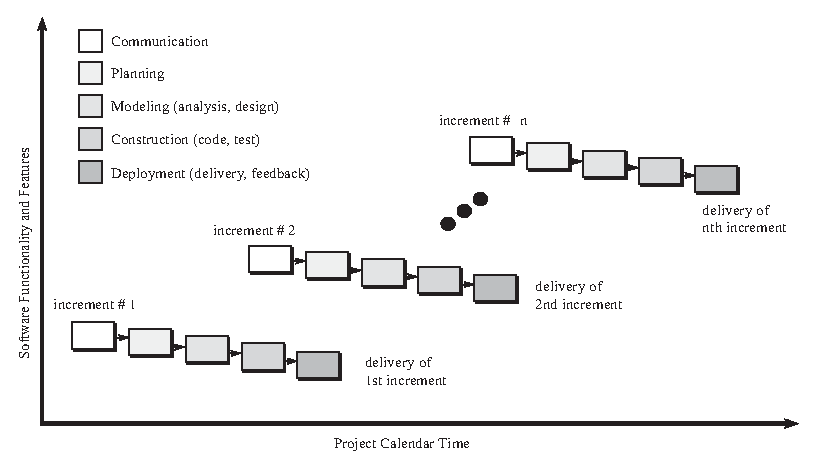
\includegraphics{Imagenes/iedevelopment.eps}
	\centering
	\caption{Metodolog�a iterativo e incremental \cite{Pressman2009}}
	\label{fig:methodie}
\end{figure}

El hecho de llevar a cabo un desarrollo iterativo permite la obtenci�n de retroalimentaci�n del producto que se esta desarrollando tempranamente y de esta manera poder refinar el trabajo en etapas posteriores del desarrollo. \cite{Victor2003, Mitchell2009, Martin1999,Alshamrani2015}.

\section{Metodolog�a de evaluaci�n}
\subsection{Casos de estudio}
Un caso de estudio \cite{Runeson2009} es una metodolog�a de investigaci�n la cual en ingenier�a de software permite analizar un proyecto, un grupo de personas, un producto, etc, en un contexto real con el objetivo de responder la pregunta de investigaci�n planteada. Esta metodolog�a de evaluaci�n considera aspectos formales para obtener evidencia. Los principales aspectos son:

\begin{itemize}
	\item Describir el contexto de aplicaci�n del caso: Consiste en establecer sobre que elemento se aplicara el caso de estudio a desarrollar.
	\item Definici�n de objetivos experimentales: Consiste en indicar cual es el objetivo de la investigaci�n a realizar, si es describir, evaluar o explicar alg�n suceso.
	\item Definici�n de un protocolo para conducir el caso de estudio: Consiste en escoger las pautas para llevar a cabo el caso de estudio, que instrumentos ser�n utilizados para recolectar datos y como se realizaran el an�lisis de estos.
	\item Definici�n de caracter�sticas a evaluar: Consiste en establecer que es lo que estamos interesados en evaluar del elemento sobre el que se aplica el caso de estudio.
	\item Definici�n de sujetos de prueba: Consiste en indicar cual sera la fuente de datos a ser utilizada para el caso de estudio, estas pueden ser personas, datos ya recolectados, etc.
	\item Aplicaci�n de caso de estudio en un conjunto de sesiones no controladas: Consiste en llevar a cabo el caso de estudio sobre los sujeto de prueba definidos.
	\item Aplicaci�n de herramientas de obtenci�n de evidencia emp�rica: Consiste en la utilizaci�n de m�todos o t�cnicas con el fin de obtener evidencia emp�rica a partir de los datos recolectados 	
	\item An�lisis y evaluaci�n de datos emp�ricos: Consiste en analizar la evidencia y evaluar la validez de los resultados obtenidos.
\end{itemize}

\section{Herramientas para la implementaci�n del software}
\subsubsection{Java}
Java es un lenguaje de programaci�n de alto nivel orientado a objetos y de prop�sito general. Un programa java se ejecuta sobre la maquina virtual llamada la Java Virtual Machine, la cual le da a este lenguaje la caracter�stica de ser multiplataforma. Adicionalmente, java incorpora el soporte para multi-hilos, una poderosa herramienta que permite la ejecuci�n de distintas instrucciones de c�digo al mismo tiempo \cite{Gosling2015}. Ademas. este lenguaje tambi�n incorpora una caracter�stica conocida como el recolector de basura, el cual se encarga de limpiar la memoria de objetos que ya no est�n siendo utilizados.  Fue anunciado por Sun Microsystems en Mayo de 1995 \cite{3java}. 

\subsubsection{Java Reflection}
Caracter�stica de java que permite que un programa se auto examine. Esta caracter�stica est� disponible a trav�s de la Java Reflection API, la cual cuenta con m�todos para obtener los meta-object de las clases, m�todos, constructores, campos o par�metros. Esta API tambi�n permite crear nuevos objetos cuyo tipo era desconocido al momento de compilar el programa \cite{Braux1999}.
\subsubsection{Java Annotation}
Caracter�stica de java para agregar metadatos a elementos de java (clases, m�todos, par�metros, etc.) [7]. Las anotaciones no tienen efecto directo sobre el c�digo, pero cuando son usadas junto con otras herramientas pueden llegar a ser muy �tiles. Estas herramientas pueden analizar estas anotaciones y realizar acciones en base a estas, por ejemplo, generar archivos adicionales como clases de java, archivos xml, entre otras; ser analizadas durante la ejecuci�n del programa v�a Java Reflection, para crear objetos cuyo tipo no conocemos en tiempo de compilaci�n; etc. 
\section{Red de distribuci�n de agua potable}
Conjunto de elementos enlazados de tal manera que permite suministrar cierta cantidad de agua a una presi�n establecida \cite{Doctoral2012}.

\subsubsection{Caudal}
Cantidad de agua que se mueve a trav�s de un segmento de la red.

\subsection{Componentes f�sicos de una red}
A continuaci�n se define los componentes que conforman una red de agua potable \cite{Rossman2017}, los cuales se aprecian en la Figura \ref{fig:componentesfisicos}:


\begin{figure}[h]
	 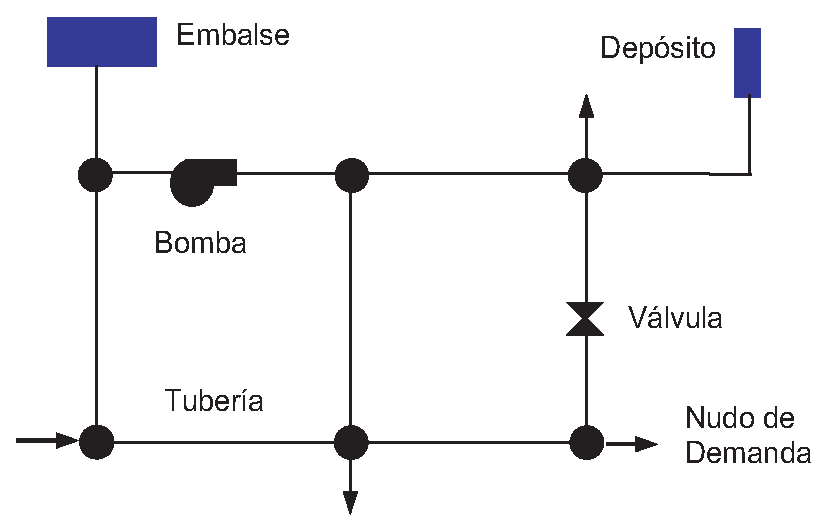
\includegraphics{Imagenes/componentesfisicosred.eps}
	\centering
	\caption{Componentes f�sicos de un sistema de distribuci�n de agua \cite{Rossman2017}}
	\label{fig:componentesfisicos}
\end{figure}
\subsubsection{Nudos de caudal}

Son los puntos o extremos de una tuber�a, los cuales tambi�n permiten que estas se unan. Estos nudos pueden actuar como nudos de demanda a trav�s de los cuales el flujo abandona la red.

\subsubsection{Embalse}
Es una fuente de alimentaci�n externa.
\subsubsection{Deposito}
Son elementos con la capacidad de almacenar agua.
\subsubsection{Tuber�a}
 Son los elementos a trav�s de los cuales transita el agua de un nudo a otro.
\subsubsection{Bomba}
Elementos que permiten impulsar el liquido con el fin de elevarlo a una posici�n superior.
\subsubsection{V�lvula}
Elementos que limitan la presi�n o el caudal que transita en un punto de la red.
\subsection{Epanet}
Software que permite simular el comportamiento hidr�ulico y la calidad del agua en redes de distribuci�n de aguas compuesta por tuber�as, nodos, bombas, v�lvulas y tanques de almacenamiento \cite{Rossman2017}.  Este software cuenta tambi�n con una librer�a din�mica conocida bajo el nombre de Epanet Programming Toolkit, la cual cuenta con un conjunto de funciones para realizar simulaciones desde diferentes entornos de desarrollo como C, C++, VB, Java, etc \cite{Rossman1999}.
\section{Optimizaci�n}
La optimizaci�n consiste en maximizar o minimizar un conjunto de funciones que matem�ticamente pueden ser expresadas de la siguiente forma:
$$f_1(x),f_2(x), ..., f_N(x),\ x=(x_1,...,x_d) | x \in X$$
sujeto a una serie de condiciones
$$h_j(x) = 0, j=1,2,...,J$$
$$g_k(x) \leq 0, k=1,2,...,K$$
siendo $f_1,...,f_N$ funciones objetivos; $x_1, ..., x_d$ variables de decisi�n, pertenecientes al espacio de b�squeda $X$; y $h_j$ junto con $g_k$, una serie de restricciones \cite{Yang2015}. De acuerdo a la cantidad de funciones objetivos que se tenga, se establece que si $N=1$ la optimizaci�n es \textbf{monoobjetivo}, mientras que para $N\geq 2$ se conoce como \textbf{multiobjetivo} \cite{Yang2015}. En este punto se debe tener en cuenta que los objetivos planteados deben encontrarse en contradicci�n. 

Debido a la definici�n de las restricciones es posible dividir el espacio de b�squeda en dos regiones \cite{Bozorg-Haddad2017}:
\begin{itemize}
	\item Soluciones factibles: Compuesto por los elementos pertenecientes al espacio de b�squeda que satisfacen todas las restricciones.
	\item Soluciones no factibles: Integrado por aquellos elementos que no complen todas las restricciones.
\end{itemize}
\section{Heur�stica}
Es el conocimiento que se tiene del problema el cual permite acotar la b�squeda de las soluciones en espacios de b�squeda de gran tama�o que hacen inviable la aplicaci�n de t�cnicas deterministas por el costo de tiempo que implican. Con la utilizaci�n de estas t�cnicas se espera encontrar soluciones buenas en un tiempo razonable, pero esto no esta garantizado \cite{Yang2015,Romanycia1985}.
\section{Metaheur�stica}
Algoritmos que permiten resolver un amplio rango de problemas de optimizaci�n empleando t�cnicas con alg�n grado de aleatoriedad para encontrar soluciones a un problema. Estos algoritmos no garantizan que la soluci�n encontrada sea la �ptima, pero permiten obtener generalmente aproximaciones a esta. La diferencia entra heur�sticas y metaheur�sticas, es que esta ultima puede ser aplicado a un amplio conjunto de problemas sin necesidad de realizar grandes cambios en el algoritmo, mientras que las heur�sticas generalmente son aplicadas a un dominio especifico \cite{Yang2015,Boussaid2013,Luke2013}.
\subsection{Algoritmos Evolutivos}
Conjunto de algoritmos inspirado en la teor�a de la evoluci�n de Darwin acerca de la capacidad de la naturaleza para evolucionar seres vivos bien adaptados a su entorno. Estos algoritmos hacen uso de diversos mecanismos entre los que se encuentra la selecci�n, mutaci�n y cruzamiento sobre los individuos de una poblaci�n con el fin de generar una nueva generaci�n de individuos \cite{Boussaid2013}. En la Figura \ref{fig:EA} muestra un un pseudocodigo de los pasos generales de un algoritmo evolutivo.


%\begin{figure}[h]
%	\begin{algorithm}[H]
%		\caption{Algoritmo Evolutivo}
%		\DontPrintSemicolon
%		\SetKwFunction{CreateInitialPopulation}{createInitialPopulation}
%		\SetKwFunction{EvaluatePopulation}{evaluatePopulation}
%		\SetKwFunction{Selection}{selection}
%		\SetKwFunction{Crossover}{crossover}
%		\SetKwFunction{Mutation}{mutation}
%		\SetKwFunction{Replace}{replace}
%		\SetKwData{PopulationVar}{population}
%		\SetKwData{SelectionVar}{selection}
%		\SetKwData{OffspringVar}{offspringPopulation}
%		
%		\PopulationVar $\leftarrow$ \CreateInitialPopulation{}\;
%		\EvaluatePopulation{\PopulationVar}\;
%		
%		\While{is not stopping condition reached}{
%			\SelectionVar $\leftarrow$ \Selection{\PopulationVar}\;
%			\OffspringVar $\leftarrow$ \Crossover{\SelectionVar}\;
%			\OffspringVar $\leftarrow$ \Mutation(\OffspringVar)\;
%			\OffspringVar $\leftarrow$ \EvaluatePopulation(\OffspringVar)\;
%			\PopulationVar $\leftarrow$ \Replace(\PopulationVar, \OffspringVar)\;
%		}
%		
%	\end{algorithm}
%	\caption{Pseudocodigo algoritmo evolutivo}
%	\label{fig:EA}
%\end{figure}

\begin{figure}[h]
	\begin{algorithm}[H]
		\caption{Algoritmo Evolutivo}
		\DontPrintSemicolon
		\SetKwFunction{CreateInitialPopulation}{crearPoblaci�nInicial}
		\SetKwFunction{EvaluatePopulation}{evaluarPoblaci�n}
		\SetKwFunction{Selection}{selecci�n}
		\SetKwFunction{Crossover}{cruzamiento}
		\SetKwFunction{Mutation}{mutaci�n}
		\SetKwFunction{Replace}{remplazar}
		\SetKwData{PopulationVar}{poblaci�n}
		\SetKwData{SelectionVar}{poblacionSeleccionada}
		\SetKwData{OffspringVar}{poblaci�nDecendiente}
		
		\PopulationVar $\leftarrow$ \CreateInitialPopulation{}\;
		\EvaluatePopulation{\PopulationVar}\;
		
		\While{la condici�n de termino no ha sido alcanzada}{
			\SelectionVar $\leftarrow$ \Selection{\PopulationVar}\;
			\OffspringVar $\leftarrow$ \Crossover{\SelectionVar}\;
			\OffspringVar $\leftarrow$ \Mutation(\OffspringVar)\;
			\OffspringVar $\leftarrow$ \EvaluatePopulation(\OffspringVar)\;
			\PopulationVar $\leftarrow$ \Replace(\PopulationVar, \OffspringVar)\;
		}
		
	\end{algorithm}
	\caption{Pseudocodigo algoritmo evolutivo}
	\label{fig:EA}
\end{figure}

Primero, se crea la poblaci�n inicial. Luego, se eval�an los objetivos de dicha poblaci�n y se itera hasta que la condici�n de termino haya sido alcanzada. La condici�n de t�rmino puede ser, por ejemplo un m�ximo numero de evaluaciones o evaluaciones sin mejoras en los resultados.  Dentro del ciclo se realiza la selecci�n sobre la poblaci�n con el fin de determinar las soluciones que ser�n usadas en los operadores de cruzamiento y mutaci�n. Finalmente, se remplaza la poblaci�n inicial con la descendiente.

\subsubsection{Poblaci�n}
Conjunto de soluciones candidatas sobre las cual opera el algoritmo. Durante cada iteraci�n del algoritmo se generan nuevas soluciones que son agregadas a la poblaci�n a la vez que se remueven otras. Una soluci�n en la poblaci�n se conoce como individuo \cite{Heiss-Czedik1997}. 

Los individuos pueden ser representados de diversas maneras, entre ellas se encuentra la representaci�n binaria (1 y 0), la real(Los n�meros reales), etc. Para la representaci�n binaria cada variable se codifica como un conjunto de bits, lo cual forma una cadena binaria. Por ejemplo, la representaci�n binaria de la soluci�n $(2,4,6,8)$ formada por enteros de 4 bits corresponder�a a

$$0010\ 0100\ 0110\ 1000$$


 En cambio, para la representaci�n real esta se presenta como un vector, en donde cada valor que forma este vector pertenece a los n�meros reales, es decir, $$v = (x1,x2, \dots, x_n), \textrm{en donde } v \in \mathbb{R}^n$$

\subsubsection{Selecci�n}
La selecci�n es un mecanismo utilizado por los algoritmos evolutivos para escoger a los individuos mas aptos los cuales ser�n usados para la reproducci�n \cite{Heiss-Czedik1997}. Existen numerosos algoritmos de selecci�n que pueden ser utilizados en los algoritmos evolutivos.


\subsubsection{Cruzamiento}
El cruzamiento es un mecanismo usado para generar nuevos soluciones a partir de dos o mas individuos seleccionados \cite{Blum2003, Boussaid2013}.
\subsubsection{Mutaci�n}
La mutaci�n es un operador el cual permite mantener la diversidad en la descendencia \cite{Boussaid2013} realizando modificaciones en ciertas partes de la soluci�n.

\subsection{Algoritmo Gen�tico}
El algoritmo gen�tico es una estrategia de b�squeda de soluciones. Para realizar esto, el algoritmo parte desde un conjunto de soluciones denominada poblaci�n he iterativamente, lleva a cabo un proceso de reproducci�n, generando nuevas soluciones \cite{Heiss-Czedik1997}. Este algoritmo pertenece a la categor�a de algoritmos evolutivos y por lo tanto puede usar el mismo esquema presentado en la Figura \ref{fig:EA}.

Los individuos en el contexto del algoritmo gen�tico son llamados cromosomas, los cuales como se menciono en la secci�n de los algoritmos evolutivos pueden ser representados de diversas maneras.

\subsection{Conceptos para la optimizaci�n multiobjetivo}
Como resultado de un proceso de optimizaci�n multiobjetivo no existe una �nica soluci�n a un problema, sino que se tiene un conjunto de soluciones. Es por ello que a continuaci�n se presentaran una serie de criterios que permitir�n analizar y determinar el conjunto de soluciones optimas. Los criterios son los siguientes \cite{VanVeldhuizen1998}:
 
\subsubsection{Dominancia de Pareto}

Sean $u$ y $v$ vectores pertenecientes a $\Re^n$, se dice que $u$ domina a $v$ (se denota como $u \preceq v$) si, y s�lo si (en el caso de minimizaci�n):
$\forall i \in \{1,2,...,n\} | f_i(u) \leq f_i(v) \wedge \exists j \in \{1,2,...,n\} | f_j(u) < f_j(v)$

Es decir, para que una soluci�n domine a otra, cada uno de sus objetivos debe ser mejores o iguales y al menos en uno de ellos este debe ser mejor.

En el ejemplo de la Figura \ref{fig:dominancia} se muestra los vectores A,B,C,D de los cuales C y B dominan a D, y A domina a C B y D. N�tese que C y B no son dominantes entre s�. 

\subsubsection{Optimo de Pareto}
Una soluci�n $u$ es un optimo de Pareto si no hay otra soluci�n $v$ en el espacio $\Omega$, tal que v domine a u, es decir, para $u , v \in \Re^n\ \  \nexists v \preceq u $. Los �ptimos de pareto tambi�n se conocen bajo el nombre de soluci�n no-dominada. En la Figura \ref{fig:dominancia} el vector A ser�a un optimo de Pareto.

\begin{figure}[h]
	 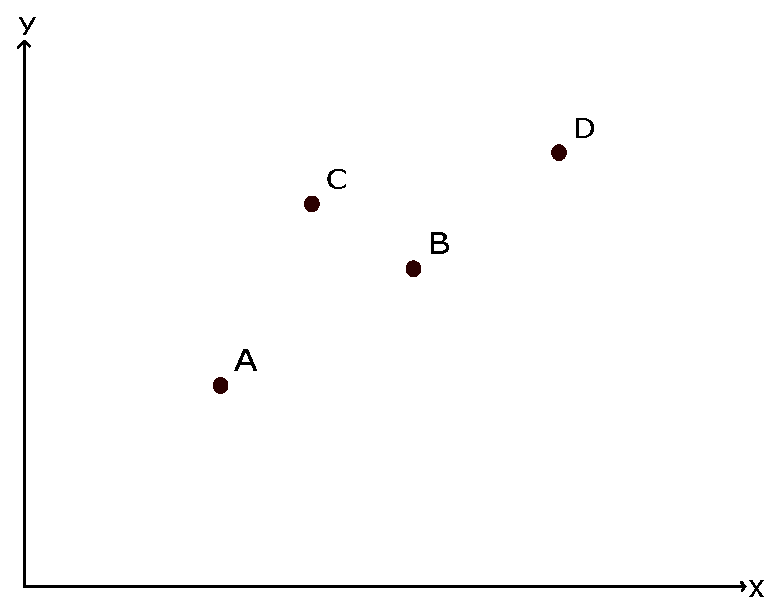
\includegraphics{Imagenes/dominancia.eps}
	\centering
	\caption{Ejemplo de dominancia y �ptimo de Pareto}
	\label{fig:dominancia}
\end{figure}

\subsubsection{Frontera de Pareto}
La frontera de Pareto es el conjunto de todas las soluciones no dominadas las cuales componen las soluciones �ptimas al problema multiobjetivo. En la Figura \ref{fig:frente_pareto} los puntos rojos componen la frontera de Pareto.

\begin{figure}[h]
	 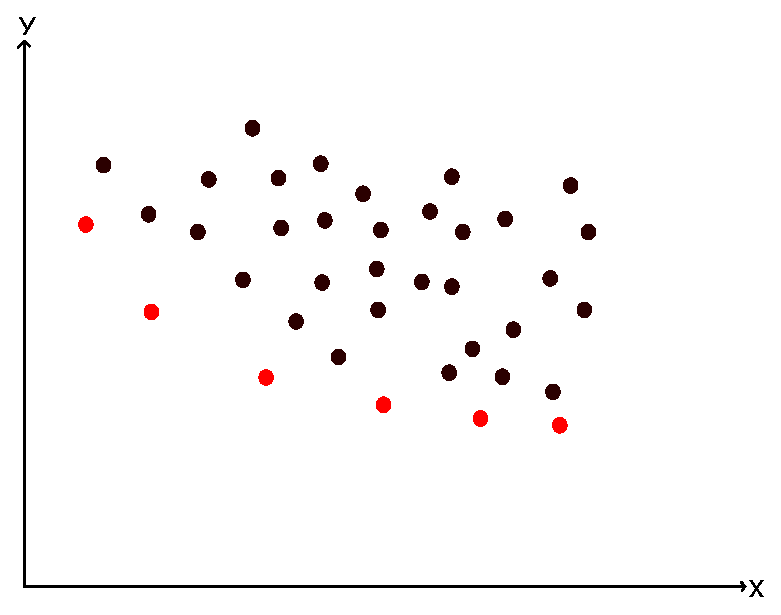
\includegraphics{Imagenes/frontera-pareto.eps}
	\centering
	\caption{Ejemplo frente de Pareto}
	\label{fig:frente_pareto}
\end{figure}
\subsection{Algoritmo NSGA-II (Nondominated Genetic Algorithm)}
El algoritmo NSGA-II \cite{Deb2002} pertenece a la categor�a de algoritmo evolutivo multiobjetivo (MOEA). Este algoritmo al igual que el algoritmo gen�tico hace uso de los operadores de selecci�n, cruzamiento y mutaci�n para encontrar un conjunto de soluciones optimas a problemas que cuentan con m�s de un objetivo. Adicionalmente, NSGA-II a�ade conceptos y operadores adicionales los cuales permiten mejorar su rendimiento y la calidad de las soluciones obtenidas. NSGA-II puede ser implementado siguiendo los mismos pasos de el algoritmo evolutivo mostrados en la Figura \ref{fig:EA}, utilizando la funci�n de remplazo mostrada en la Figura \ref{fig:RemplaceNSGAII}.

En la Figura \ref{fig:RemplaceNSGAII} se puede ver que el proceso de remplazo dentro del algoritmo gen�tico consiste en unir la poblaci�n actual y la poblaci�n descendiente (formada por los elementos resultantes del operador de selecci�n y sobre la que se han aplicado el cruzamiento y la mutaci�n) en un solo elemento llamada unionPoblaci�n. Luego, esta  es enviada a un procedimiento el cual ordena y categoriza la poblaci�n en diversos frentes de acuerdo al concepto de dominancia de Pareto. Despu�s, de que la poblaci�n a sido categorizada se procede a iterar sobre los frentes y a�adir sus elementos a una nueva poblaci�n con el cuidado de no sobrepasar el tama�o de la poblaci�n deseada ($N$). En caso de que uno de los frentes no pueda ser a�adido en su totalidad por sobrepasar dicho tama�o, se llevar� a cabo un proceso por el cual se ordenaran las soluciones en dicho frente basadas en un criterio conocido como densidad de las soluciones. Una vez realizado el ordenamiento, se agregar�n las mejores soluciones a la nueva poblaci�n hasta alcanzar el tama�o deseado  $N$. Se puede ver un ejemplo de este procedimiento gr�ficamente en la Figura \ref{fig:procedimientoNSGAII}.

% Una vez las soluciones se encuentren ordenadas se rellenar� la nueva poblaci�n hasta alcanzar el tama�o de deseado $N$. 

\begin{figure}[h]
	\begin{algorithm}[H]
		\caption{Funci�n de remplazo para el algoritmo NSGA-II}
		\DontPrintSemicolon
		\SetKwData{PopulationVar}{poblaci�n}
		\SetKwData{OffspringVar}{poblaci�nDescendiente}
		\SetKwData{JoinVar}{unionPoblacion}
		\SetKwData{Front}{$F$}
		\SetKwData{NewPopulation}{nuevaPoblacion}

		\SetKwFunction{FastNonDominatingSorting}{ordenarPorFrentesNoDominados}
		\SetKwFunction{CrowdingDistanceAssignament}{asignarDensidad}
		\SetKwFunction{Sort}{ordernar}

		\SetKwProg{Fn}{Function}{}{fin}
		\Fn{remplazar(\PopulationVar, \OffspringVar)}{
		
		$\JoinVar \leftarrow \PopulationVar \cup \OffspringVar$\;
		\BlankLine
		\tcc*[h]{$F = (F_1,F_2, ...)$}\;
		\Front $\leftarrow$ \FastNonDominatingSorting(\JoinVar)\;
		\BlankLine
		\NewPopulation $\leftarrow \emptyset$ \;
		\BlankLine
		$i = 1$\;
		\BlankLine
		\tcc*[h]{Hasta que \NewPopulation este lleno}\;
		\While{$(|\NewPopulation| +|F_i|) \leq N$}{
			\tcc{Calcular y asignar la densidad a cada soluci�n del frente $F_i$}
			\CrowdingDistanceAssignament($F_i$)\;
			\BlankLine
			\tcc{A�adir a \NewPopulation las soluciones del frente $F_i$}
			\NewPopulation $\leftarrow$ \NewPopulation $\cup$ $F_i$ \;
			\BlankLine
			$i = i+1$\;
		}
		\BlankLine
		\tcc{Ordenar el frente $F_i$ usando el comparador de densidad}
		\Sort($F_i$, $\prec_n$) \;
		\BlankLine
		\tcc{Elegir los primeros $N -|\NewPopulation|]$ }
		\NewPopulation $\leftarrow$ \NewPopulation $\cup$ $F_i[1: N -|\NewPopulation|]$ \;
		\BlankLine
		retornar \NewPopulation\;
	}
		
	\end{algorithm}
	\caption{Pseudoc�digo de la funci�n de remplazo utilizada en el algoritmo NSGA-II \cite{Deb2002}}
	\label{fig:RemplaceNSGAII}
\end{figure}


\begin{figure}[h]
	 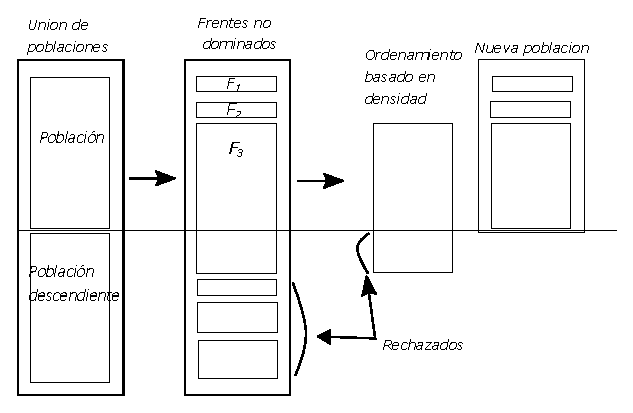
\includegraphics{Imagenes/ProcedimientoNSGA-II.eps}
	\centering
	\caption{Procedimiento NSGA-II \cite{Deb2002}}
	\label{fig:procedimientoNSGAII}
\end{figure}

A continuaci�n se proceder� a explicar los operadores adicionales presentados en \cite{Deb2002} y que son utilizados por la funci�n de remplazo del algoritmo NSGA-II en la Figura \ref{fig:RemplaceNSGAII}.

\subsubsection{Ordenamiento de soluciones en frentes no dominados}
Uno de los procedimientos presentados en la Figura \ref{fig:RemplaceNSGAII} consiste en ordenar las soluciones en frentes no dominados. Los frentes no dominados son conjuntos en los que se almacenan las soluciones que no se dominan entre si. En la Figura \ref{fig:frente-no-dominados} se muestra un ejemplo con tres frentes.

\begin{figure}[h]
	 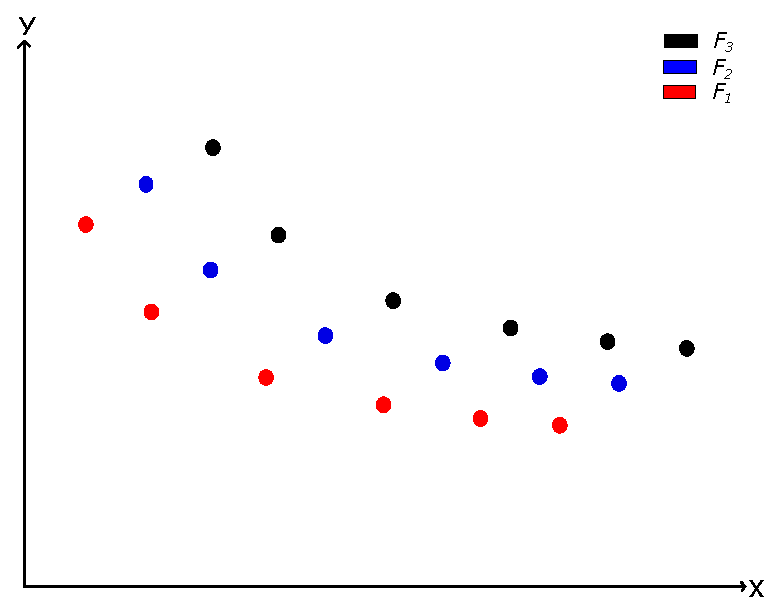
\includegraphics{Imagenes/frentes-no-dominados.eps}
	\centering
	\caption{Frentes no dominados}
	\label{fig:frente-no-dominados}
\end{figure}

El algoritmo para llevar a cabo esto se presenta en la Figura \ref{fig:sortFront} y consiste en lo siguiente:

Primero, se debe comparar todas las soluciones entre si utilizando el concepto de dominancia de Pareto. Para ello, cada soluci�n $p$ cuenta con un atributo $S_p$ en el que guarda todas las soluciones a las que domina y un contador $n_p$ que almacena el numero de soluciones que lo dominan a �l. Cada vez que se termina de comparar una soluci�n con todas las otras, si su contador $n_p$ es igual a 0, se le asigna a la soluci�n el rango que indica el frente al que pertenece, y se guarda esta en un conjunto que contiene a todas las soluciones de dicho frente $F_1$. 
	
Una vez que se han identificado todas las soluciones no dominadas del primer frente se procede a generar el siguiente, para lo cual, por cada soluci�n $q$ almacenada en el conjunto $S_p \in p$ del frente ya conocido se disminuye en uno su contador $n_q$. Si el contador $n_q$ de la soluci�n $q$ llega a 0, entonces se le asigna a dicha soluci�n el rango correspondiente y se guarda esta en un conjunto temporal $Q$ con el resto de las soluciones en dicho frente. Cuando se tengan identificadas todas las soluciones, estas se asignan al frente correspondiente $F_i$. 

Finalmente, se repite el procedimiento anterior sobre el nuevo frente hasta haberlos generado todos.


\begin{figure}[h]
	\begin{algorithm}[H]
		\caption{Funci�n de ordenaci�n en frentes no dominados}
		\DontPrintSemicolon
		\SetKwData{PopulationVar}{poblaci�n}
		\SetKwData{Front}{$F$}
		\SetKwData{NewPopulation}{nuevaPoblacion}
		
		\SetKwFunction{FastNonDominatingSorting}{ordenarPorFrentesNoDominados}


		
		\SetKwProg{Fn}{Function}{}{fin}
		\Fn{\FastNonDominatingSorting(\PopulationVar)}{
		$\Front \leftarrow \emptyset$\;
		\ForEach{$p \in \PopulationVar$}{
			\tcc*[h]{Conjunto de soluciones dominadas por $p$}\;
			$S_p = \emptyset$\; 
			\tcc*[h]{Numeros de soluciones que dominan a $p$}\;
			$n_p = 0$\;
			\ForEach{$q \in \PopulationVar$}{
				\uIf(\tcc*[h]{$p$ domina a $q$}){$p \prec q$}{
					$S_p = S_p \cup \{q\}$\;
				}\ElseIf(\tcc*[h]{$q$ domina a $p$}){$q \prec p$}{
					$n_p = n_p + 1$\;
				}
				\If{$n_p = 0$}{
					$p_{rango} = 1$\;
					$F_1 = F_1 \cup \{p\}$\;
				}	
			}
		}
		\BlankLine
		$i = 1$\;
		\BlankLine
		\While{$F_i \neq 0$}{
			$Q = \emptyset$\;
			\ForEach{$p \in \Front_i$}{
				\ForEach{$q \in S_p$}{
					$n_q = n_q - 1$\;
					\If{$n_q = 0$}{
						$q_{rango} = i + 1$\;
						$Q = Q \cup \{q\}$\;
					}
				}
			}

			$i = i+1$\;
			$F_i = Q$\;
		}
		
		
		
	}
		
	\end{algorithm}
	\caption{Pseudoc�digo de la funci�n de ordenamiento utilizada en NSGA-II \cite{Deb2002}}
	\label{fig:sortFront}
\end{figure}

\subsubsection{Densidad de estimaci�n (Crowing Distance)}
Otra funci�n presente en la Figura \ref{fig:RemplaceNSGAII} es la asignaci�n de las densidades sobre cada soluci�n, la cual corresponde a la distancia promedio entre la soluci�n anterior y la siguiente a partir de cada uno de los objetivos. En la Figura \ref{fig:crowdingDistance} la densidad de la soluci�n $i$ corresponde a la suma de la longitud del lado mayor y del lado menor del rect�ngulo.

\begin{figure}[h]
	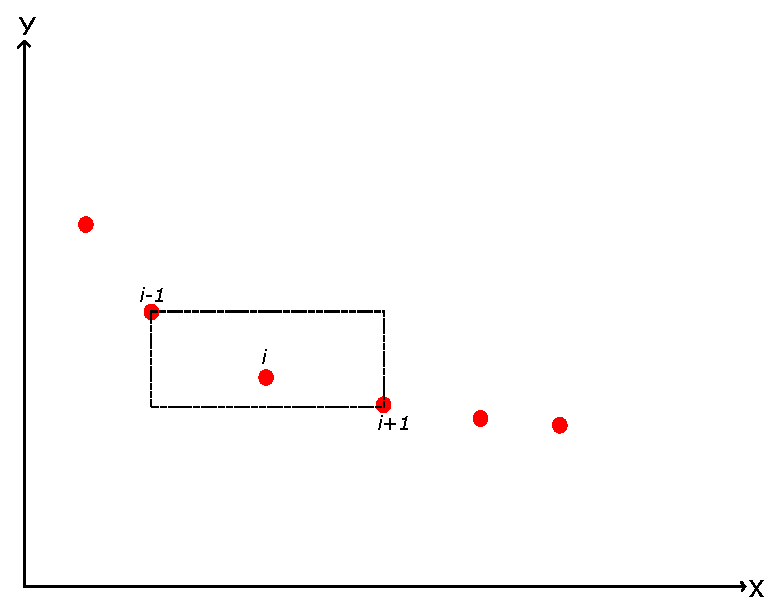
\includegraphics[scale=0.8]{Imagenes/crowing-distance.eps}
	\centering
	\caption{Calculo de la densidad de estimaci�n al rededor de la soluci�n $i$ \cite{Deb2002}.}
	\label{fig:crowdingDistance}
\end{figure}

El procedimiento para esta funci�n  se muestra en la Figura \ref{fig:crowdingDistance} y consiste en:

Primero, crear e inicializar un arreglo $\mathcal{I}_{distancia}$, con el valor 0, en donde guardar las distancias para cada soluci�n a medida que se van calculando. Luego, por cada uno de los objetivos se ordena el frente $\mathcal{I}$ y dentro $\mathcal{I}_{distancia}$ se le asigna al primer y ultimo elemento el valor infinito. Finalmente, se recorre desde la segunda hasta la pen�ltima soluci�n calculando la distancia $\mathcal{I}[i]_{distancia}$. Notar que $f_m^{max}$ y $f_m^{min}$ corresponden al valor del objetivo $m$ de la primera y ultima soluci�n.

\begin{figure}[h]
	\begin{algorithm}[H]
	\caption{Funci�n de calculo de densidades}
	\DontPrintSemicolon
	\SetKwData{NDS}{$\mathcal{I}$}
	\SetKwFunction{CrowdingDistanceAssignament}{asignarDensidad}
		
		
		
	\SetKwProg{Fn}{Function}{}{fin}
	\Fn(\tcc*[h]{$\NDS$ : frente de soluciones no dominadas}){\CrowdingDistanceAssignament($\NDS$)}{
		$l = |\NDS|$ \tcc*[h]{Obtiene el tama�o del frente}\;\;
		\BlankLine
		\tcc*[h]{Inicializa la distancia para cada soluci�n}\;
		\ForEach{$i \leftarrow 1$ \KwTo $l$}{
			$\NDS[i]_{distancia} \leftarrow 0$
		}
		\ForEach{$m \leftarrow 1$ \KwTo numero de objetivos}{
			$\NDS \leftarrow$ sort($\NDS$, m) \tcc*[h]{Ordena por el objetivo m}\; 
			\BlankLine
			\tcc*[h]{Asignar a la primera y ultima solucion el valor $\infty$ }\;
			$\NDS[1]_{distancia} \leftarrow \NDS[l]_{distancia} \leftarrow \infty$\;
			\BlankLine
			\For{$i \leftarrow 2$ \KwTo $l-1$}{
				\tcc*[h]{Asigna la distancia a las soluciones restantes}\;
				$\NDS[i]_{distancia} \leftarrow \NDS[i]_{distancia} + (\NDS[i+1].m - \NDS[i-1].m)/(f_m^{max} - f_m^{min})$\;	
			}
		}
	
	}
		
	\end{algorithm}
	\caption{Pseudoc�digo de la funci�n de asignaci�n de densidad \cite{Deb2002}}
	\label{fig:CrowindDistance}
\end{figure}
\subsubsection{Comparador de densidad (Crowing Distance comparator)}
Este operador compara las soluciones basados en dos conceptos los cuales son el rango de dominaci�n y la densidad de soluciones. Estos fueron calculados al momento de generar los frentes y asignar la densidad a las soluciones. De acuerdo a Deb \cite{Deb2002}, se define el orden dado por el operador de densidad ($\prec_n$) como: $i \prec_n j $, si $(i_{rango} < j_{rango})$ o $((i_{rango} = j_{rango})$ o $(i_{distancia} > j_{distancia}))$.

%% contenido del tercer cap�tulo
\chapter{Metodolog�a de desarrollo}
En este cap�tulo se presenta la metodolog�a a seguir durante el desarrollo del proyecto, as� como las fases que la componen y las tareas que son realizadas por cada una de estas fases.

La metodolog�a escogida para utilizar durante el desarrollo de este proyecto es la metodolog�a iterativa e incremental. Debido a que la metodolog�a esta pensada para ser llevada a cabo por un equipo de trabajo, esta se ha adaptado para poder ser aplicada en el desarrollo llevado a cabo por una sola persona. Esta adaptaci�n consiste, de manera general, en disminuir la cantidad de documentaci�n generada por cada fase, flexibilidad para permitir llevar a cabo m�s de una fase dentro de cada iteraci�n al mismo tiempo y que los roles de analista, dise�ador, implementador y tester sean realizados por una sola persona.

Las tareas a desempe�ar por cada fase consisten en:
\paragraph{An�lisis:}
\begin{itemize}
	\item Identificaci�n y especificaci�n de los requisitos de usuario. 
	\item Priorizaci�n de los requisitos.
	\item Validaci�n de requisitos.
	\item Especificaci�n formal de requisitos.
\end{itemize}
\paragraph{Dise�o:} 
\begin{itemize}
	\item Definici�n y especificaci�n de la arquitectura del sistema.
	\item Dise�o de las interfaces de usuario.
	\item Dise�o de los componentes.
	\item Especificaci�n formal del dise�o del sistema.
\end{itemize}
\paragraph{Implementaci�n:}
\begin{itemize}
	\item Programaci�n de los componentes de software.
	\item Integraci�n de los componentes de software.
	\item Elaboraci�n del producto entregable.
	\item Elaboraci�n de manual de usuario.
\end{itemize}
\paragraph{Pruebas:}
\begin{itemize}
	\item Verificaci�n del producto entregable.
	\item Definici�n y especificaci�n de casos de prueba.
	% \item Validaci�n del producto.
	% \item Registro de incidencias.
	\item Especificaci�n formal de pruebas.
\end{itemize}

Cada una de las fases mencionadas anteriormente tiene como resultado un documento de especificaci�n formal. Espec�ficamente, estos contienen el siguiente contenido:

\paragraph{Especificaci�n formal de requisitos:}
\begin{itemize}
	\item Introducci�n: En este apartado del documento se da una introducci�n al problema que se ha identificado.
	\item Requisitos de usuario: Consiste en la recopilaci�n de lo requisitos de los usuarios que deben ser cumplidos al final del periodo de desarrollo.
	\item Requisito de sistema: Son los requisitos, desde un punto de vista mas t�cnico, que son necesarios para satisfacer los requisitos de usuario.
	\item Matriz de trazado requisitos de usuario vs sistema: Matriz que permite ver la trazabilidad de los requisitos de usuario con los de sistema.
\end{itemize}
\paragraph{Especificaci�n formal del dise�o del sistema:}
\begin{itemize}
	\item Casos de uso: Serie de diagramas que permiten ver la interacci�n que el usuario tiene con el sistema.
	\item Arquitectura f�sica: Descripci�n de los componentes f�sicos que intervienen en la aplicaci�n.
	\item Arquitectura l�gica: Descripci�n a alto nivel del software y los componentes que lo componen.
	\item Diagrama de componentes: Permite ver la divisi�n del sistema y la interacci�n entre los distintos componentes~\cite{Bell2004}.
	\item Dise�o de interfaces: Bosquejos o implementaci�nes de las interfaces a ser utilizadas en la propuesta.
	\item Diagrama de clases: Describe la relaci�n entre las distintas clases presentes en la soluci�n propuesta.
\end{itemize}
\paragraph{Manual de usuario:} Explicaci�n acerca de la capacidades de la aplicaci�n, acompa�ada de esquemas y ejemplos de uso.
\paragraph{Especificaci�n formal de pruebas:} 
\begin{itemize}
	\item Se documenta las pruebas automatizadas que se realizan y sobre que elemento se llevan a cabo.
\end{itemize}

La raz�n por la que se utiliza esta metodolog�a sobre otras es porque el producto resultante de este proyecto esta pensado para servir como base para futuros trabajos. Debido a esto es necesario documentar correctamente los detalles de la implementaci�n para que otros programadores puedan continuar con su desarrollo en el futuro. Aunque existen otras metodolog�as como cascada u otras tradicionales, estas son dif�ciles de llevar a cabo por la cantidad de documentaci�n que se requiere, mientras que metodolog�as de desarrollo �gil carecen en cuanto a la documentaci�n que se necesita para el sistema a desarrollar. Adicionalmente, esta metodolog�a nos permite obtener una retroalimentaci�n al final de cada iteraci�n, obtener nuevos requisitos que no hayan quedado definidos en etapas anteriores o refinar los requisitos y el dise�o ya existente, permitiendo as� mejorar la calidad del producto final.

La implementaci�n de esta metodolog�a para el desarrollo del proyecto se lleva a cabo repartiendo las tareas necesarias para el cumplimiento de los objetivos en iteraciones. De este modo al final de cada iteraci�n se cuenta con un prototipo funcional de la aplicaci�n sobre el que se agrega las nuevas funcionalidades en las iteraciones siguientes.

\chapter{Desarrollo}
En esta cap�tulo se da a conocer la concepci�n del proyecto y como se lleva a cabo la aplicaci�n de la metodolog�a en el desarrollo de �ste. Para esto, se presenta por cada una de las fases del desarrollo las actividades realizadas en cada iteraci�n utilizando una serie de casos de prueba a modo de ejemplos de las funcionalidades a implementar. 

\section{Concepci�n del proyecto}

Este proyecto se origina como una propuesta por parte del profesor del departamento de Ingenier�a en Obras Civiles, Daniel Mora Melia. �l, junto a un grupo de expertos de diversas �reas, presentaron y publicaron un articulo del proyecto JHawanet~\cite{JHawanet-2019}. Dicho articulo, presenta la integraci�n de dos librer�as independientes, JMetal y Epanet, como herramienta para llevar a cabo optimizaciones sobre RDA. JMetal~\cite{Durillo2010} es un Framework de Java, orientado a la optimizaci�n multiobjetivo y es usado como motor de optimizaci�n. Mientras que Epanet~\cite{Rossman1999} es una herramienta la cual permite realizar simulaciones en redes de agua potable.

Debido al articulo anteriormente mencionado, surgi� la idea de crear una herramienta gr�fica con el fin de facilitar la optimizaci�n de redes de agua potable. Puesto que la utilizaci�n de la herramienta JHawanet requiere conocimiento computacional avanzado. Y de esta forma, permitir el trabajo de Ingenieros hidr�ulicos en un entorno especialmente dise�ado para su �rea sin perder la capacidad que la herramienta posee para que usuarios avanzados puedan incorporar y evaluar nuevos problemas y algoritmos. 


\section{Funcionalidades}

En esta secci�n se presentan las funcionalidades que se utilizan para demostrar la aplicaci�n de la metodolog�a.

Se escogen 3 funcionalidades las cuales corresponden a:
\paragraph{Funcionalidad 1:} El sistema debe poder visualizar la red. Esta funcionalidad consiste en visualizar gr�ficamente la forma de la red cargada. El archivo de descripci�n de red debe ser creado desde la aplicaci�n Epanet y tener la extensi�n inp.

\paragraph{Funcionalidad 2:} El sistema debe poder encontrar soluciones al problema de la optimizaci�n del dise�o de RDA basado en la selecci�n de di�metros de tuber�as utilizando un Algoritmo Gen�tico.

\paragraph{Funcionalidad 3:}  El sistema debe poder realizar una simulaci�n hidr�ulica utilizando los valores por defecto del archivo de red.
\section{Requisitos}

Durante la fase de requisitos se llevo a cabo la captura, priorizaci�n y la especificaci�n formal de requisitos.

Los requisitos iniciales de la aplicaci�n fueron capturados a partir de una reuni�n con el profesor Jimmy Gutierrez. Posteriormente, estos requisitos fueron priorizados para finalmente ser documentados en el documento de especificaci�n formal de requisitos. 

A medida que avanzaban las iteraci�nes algunos requisitos fueron cambiando o fueron surgiendo requisitos nuevos. En el Cuadro~\ref{fig:cambios_requisitos} se detallan los cambios y actividades realizados durante cada iteraci�n.

\begin{table}[H]
  \begin{center}
    \caption{Actividades y cambios de la fase de requisitos durante cada iteraci�n}
    \bigskip
    \begin{tabular}{||c| m{2cm}| m{8cm}||} 
      \hline
      \textbf{N� Iteraci�n} & \textbf{Requisitos cubiertos} & \textbf{Tareas}\\ [0.5ex] 
      \hline\hline
      1 & 5/32 & Se capturan 5 requisitos.\newline Se crea el informe de especificaci�n de requisitos. \\
      \hline
      2 & 11/32 & Se capturan 6 nuevos requisitos. \newline Se actualiza el documento de requisitos.\\
      \hline
      3 & 16/32 & Se capturan 5 nuevos requisitos. \newline Se actualiza el documento de requisitos. \\
      \hline
      4 & 20/32 & Se capturan 4 nuevos requisitos.\newline Se actualiza el documento de requisitos. \\
      \hline
      5 & 20/32 & No hay nuevos requisitos. \\
      \hline
      6 & 32/32 & Se capturan 12 nuevos requisitos.\newline Se actualiza el documento de requisitos. \\
      \hline

    \end{tabular}
   \label{fig:cambios_requisitos}
 \end{center}
\end{table}

Los cuadros~\ref{fig:RU004},~\ref{fig:RU002} y~\ref{fig:RU020} muestran la especificaci�n formal de los requisitos relacionados a las funcionalidades escogidas anteriormente.

\begin{requisito}[fig:RU004][Especificaci�n del requisito de usuario RU004.]
  \Requisito{RU004}{Visualizar red en una interfaz gr�fica.}
  \Descripcion{Se debe mostrar en la interfaz gr�fica una representaci�n de la red (Un dibujo, etc) generada a partir de la informaci�n contenida en el archivo inp.}
  
  \Fuente{Jimmy Guti�rrez}
  \Prioridad{Moderada}
  \Estabilidad{Intransable}
  \FechaA{09/09/2019}
  \Estado{Cumple}
  \Incremento{3}
  \Tipo{Funcional}
\end{requisito}

\begin{requisito}[fig:RU002][Especificaci�n del requisito de usuario RU002.]
  \Requisito{RU002}{Resolver el problema monoobjetivo (\textit{Pipe Optimizing})  usando un Algoritmo Gen�tico.}
  \Descripcion{El Algoritmo Gen�tico debe ser aplicado para resolver el problema monoobjetivo que tiene como funci�n objetivo el costo de inversi�n y como variable de decisi�n el di�metro de las tuber�as.}
  
  \Fuente{Jimmy Guti�rrez}
  \Prioridad{Alta}
  \Estabilidad{Intransable}
  \FechaA{09/09/2019}
  \Estado{Cumple}
  \Incremento{2}
  \Tipo{Funcional}
\end{requisito}

\begin{requisito}[fig:RU020][Especificaci�n del requisito de usuario RU020.]
  \Requisito{RU020}{Permitir realizar simulaciones hidr�ulicas utilizando los valores por defectos que vienen en el archivo inp y visualizar los resultados.}
    \Descripcion{Utilizando los valores que vienen por defecto en el archivo inp se debe poder llevar a cabo la simulaci�n hidr�ulica de la red. Posteriormente, los resultados podr�n ser visualizados por el usuario.}
    
    \Fuente{Daniel Mora-Meli�}
    \Prioridad{Alta}
    \Estabilidad{Intransable}
    \FechaA{27/01/2020}
    \Estado{Cumple}
    \Incremento{5}
    \Tipo{Funcional}
\end{requisito}

La especificaci�n formal de los requisitos restantes se encuentra en el \textbf{Anexo~\ref{appendix:requisito}}.






\section{Dise�o}

Una vez terminada la fase de requisitos se procede a dise�ar la aplicaci�n. Dentro del dise�o, se encuentran las tareas de escoger  y documentar la arquitectura f�sica y l�gica, realizar los diagramas de clases, diagramas de secuencia, dise�o de interfaces, entre otros.

Mientras avanzaba el desarrollo fue necesario ir modificando el documento de dise�o debido a la aparici�n o al cambio de requisitos, as� como la realizaci�n de mejoras en los diagramas realizados. En el Cuadro~\ref{fig:cambios_diseno} se presentan m�s detalladamente los cambios realizados en cada iteraci�n.

\begin{table}
  \begin{center}
    \caption{Actividades y cambios en la fase de dise�o durante cada iteraci�n}
    \begin{tabular}{||c| m{6cm}| m{6cm}||} 
      \hline
      N� Iteraci�n & Tareas & Comentario\\ [0.5ex] 
      \hline\hline
      1 & Crear arquitectura l�gica. \newline Crear arquitectura f�sica. \newline Dise�ar m�dulos.\newline Crear diagrama de clases del modulo metaheur�stica. \newline Crear diagrama de clases del la representaci�n de la red.
      & Durante esta iteraci�n se creo el documento de dise�o y se crearon los esquemas b�sicos para orientar la construcci�n del software.\\
      \hline
      2 & No hubieron cambios & No hubieron cambios en esta iteraci�n en el aspecto del dise�o.\\
      \hline
      3 & Dise�ar interfaces de usuario.\newline Especificar detalles de la implementaci�n referente a las anotaciones de Java (\textit{Java Annotations}) y \textit{Java Reflection}.\newline Generar diagrama de secuencia de optimizaci�n. & Durante esta fase de dise�aron algunas de las interfaces de usuario de la aplicaci�n. \newline Los diagramas de secuencia creados indican la interacci�n entre las clases para poder realizar una tarea.\\
      \hline
      4 & No hubieron cambios & No hubieron cambios en esta iteraci�n en el aspecto del dise�o.\\
      \hline
      5 & Modificar interfaces de usuario. \newline Crear diagrama de secuencia para realizar la simulaci�n usando las configuraciones por defecto. Modificar y mejora del diagrama de secuencia de la optimizaci�n. & Debido a requisitos del usuario en el �rea de usabilidad de la aplicaci�n fue necesario modificar las interfaces.\\
      \hline
      6 & Modificar y mejora del diagrama de secuencia de la optimizaci�n. & Se modifico el diagrama de secuencia de la optimizaci�n debido a la aparici�n de un nuevo requisito.  \\
      \hline
    \end{tabular}
    \label{fig:cambios_diseno}
  \end{center}
\end{table}

Como una de las primeras tareas realizadas durante esta fase se procedi� a definir la arquitectura de la aplicaci�n, tanto desde el punto f�sico como el l�gico. 

La arquitectura f�sica del programa a desarrollar es la arquitectura monol�tica, cuya caracter�stica es que software que posee esta arquitectura funciona localmente sin necesidad de interactuar con otros equipos. Esta elecci�n se debe a que en reuniones con el cliente se estableci� que el programa ser� usado localmente y debe operar sobre el sistema operativo Windows. Limitaci�n debida principalmente al acceso a funciones nativas cuando se realizan simulaciones hidr�ulicas utilizando la  librer�a din�mica de Epanet. La Figura~\ref{fig:arq_fisica} muestra el diagrama de la arquitectura monol�tica.

\begin{figure}[h]
  
\includegraphics[width=0.5\textwidth]{Capitulo4/assets/arquitectura_fisica.png}
  \centering
  \caption{Arquitectura f�sica monol�tica}
  \label{fig:arq_fisica}
\end{figure}

En cuanto a la arquitectura l�gica se escogi� utilizar Modelo-Vista-Controlador. �sta elecci�n es debido al hecho de que dicha arquitectura nos permite separar la capa de interfaz de usuario de la l�gica de la aplicaci�n mejorando asi escalabilidad y mantenibilidad del software. La Figura~\ref{fig:arq_logica} muestra el diagrama de la arquitectura l�gica, as� como los principales m�dulos de la aplicaci�n.

\begin{figure}[h]
  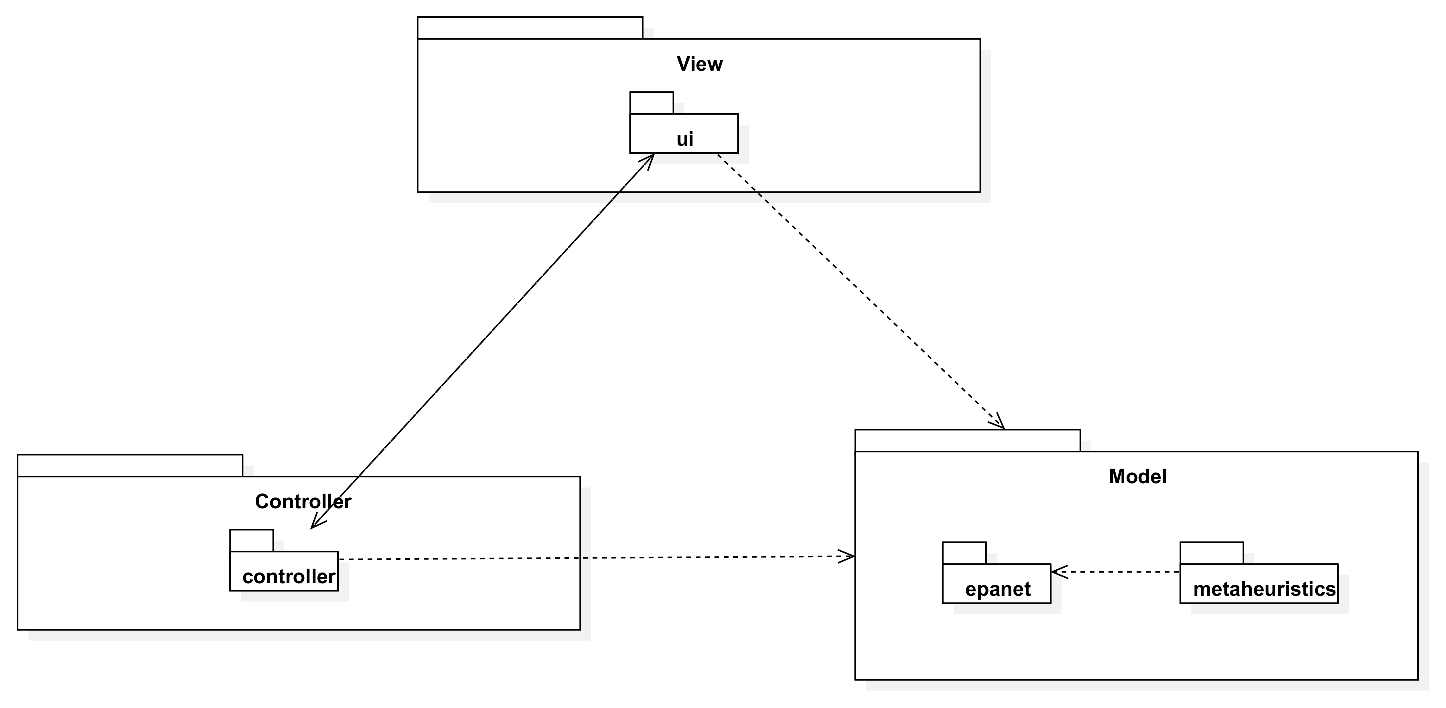
\includegraphics[width=\textwidth]{Capitulo4/assets/arquitectura_logica.eps}
  \centering
  \caption{Arquitectura l�gica Modelo-Vista-Controlador}
  \label{fig:arq_logica}
\end{figure}

A continuaci�n se presentar�n los dise�os relaci�nados por cada una de las funcionalidades escogidas con anterioridad.

\paragraph{Funcionalidad 1:} Para implementar esta funcionalidad es necesario abstraer en un conjunto de clases los datos almacenados en el archivo de configuraci�n de red. La Figura~\ref{fig:dia_clase_network} muestra el diagrama de clases reducido (se dejan fuera varias clases que especifican las configuraciones generales de la red) de la estructura sobre la que se almacenan los datos al momento de cargar la red. La clase \textit{Network} act�a como un contenedor para las dem�s clases presentes en el diagrama.


\begin{figure}[h]
  \centering
  \includegraphics[width=\textheight, angle=90]{Capitulo4/assets/d_clases_network.eps}
  \caption{Diagrama de clases de la abstracci�n de la red reducido.}
  \label{fig:dia_clase_network}
\end{figure}

El diagrama de la Figura~\ref{fig:dia_sec_visualizacion} muestra el conjunto de clases y los mensajes de la clases que interact�an con la clase \textit{Network} con el fin de visualizar la red. 

\begin{figure}[h]
  \centering
  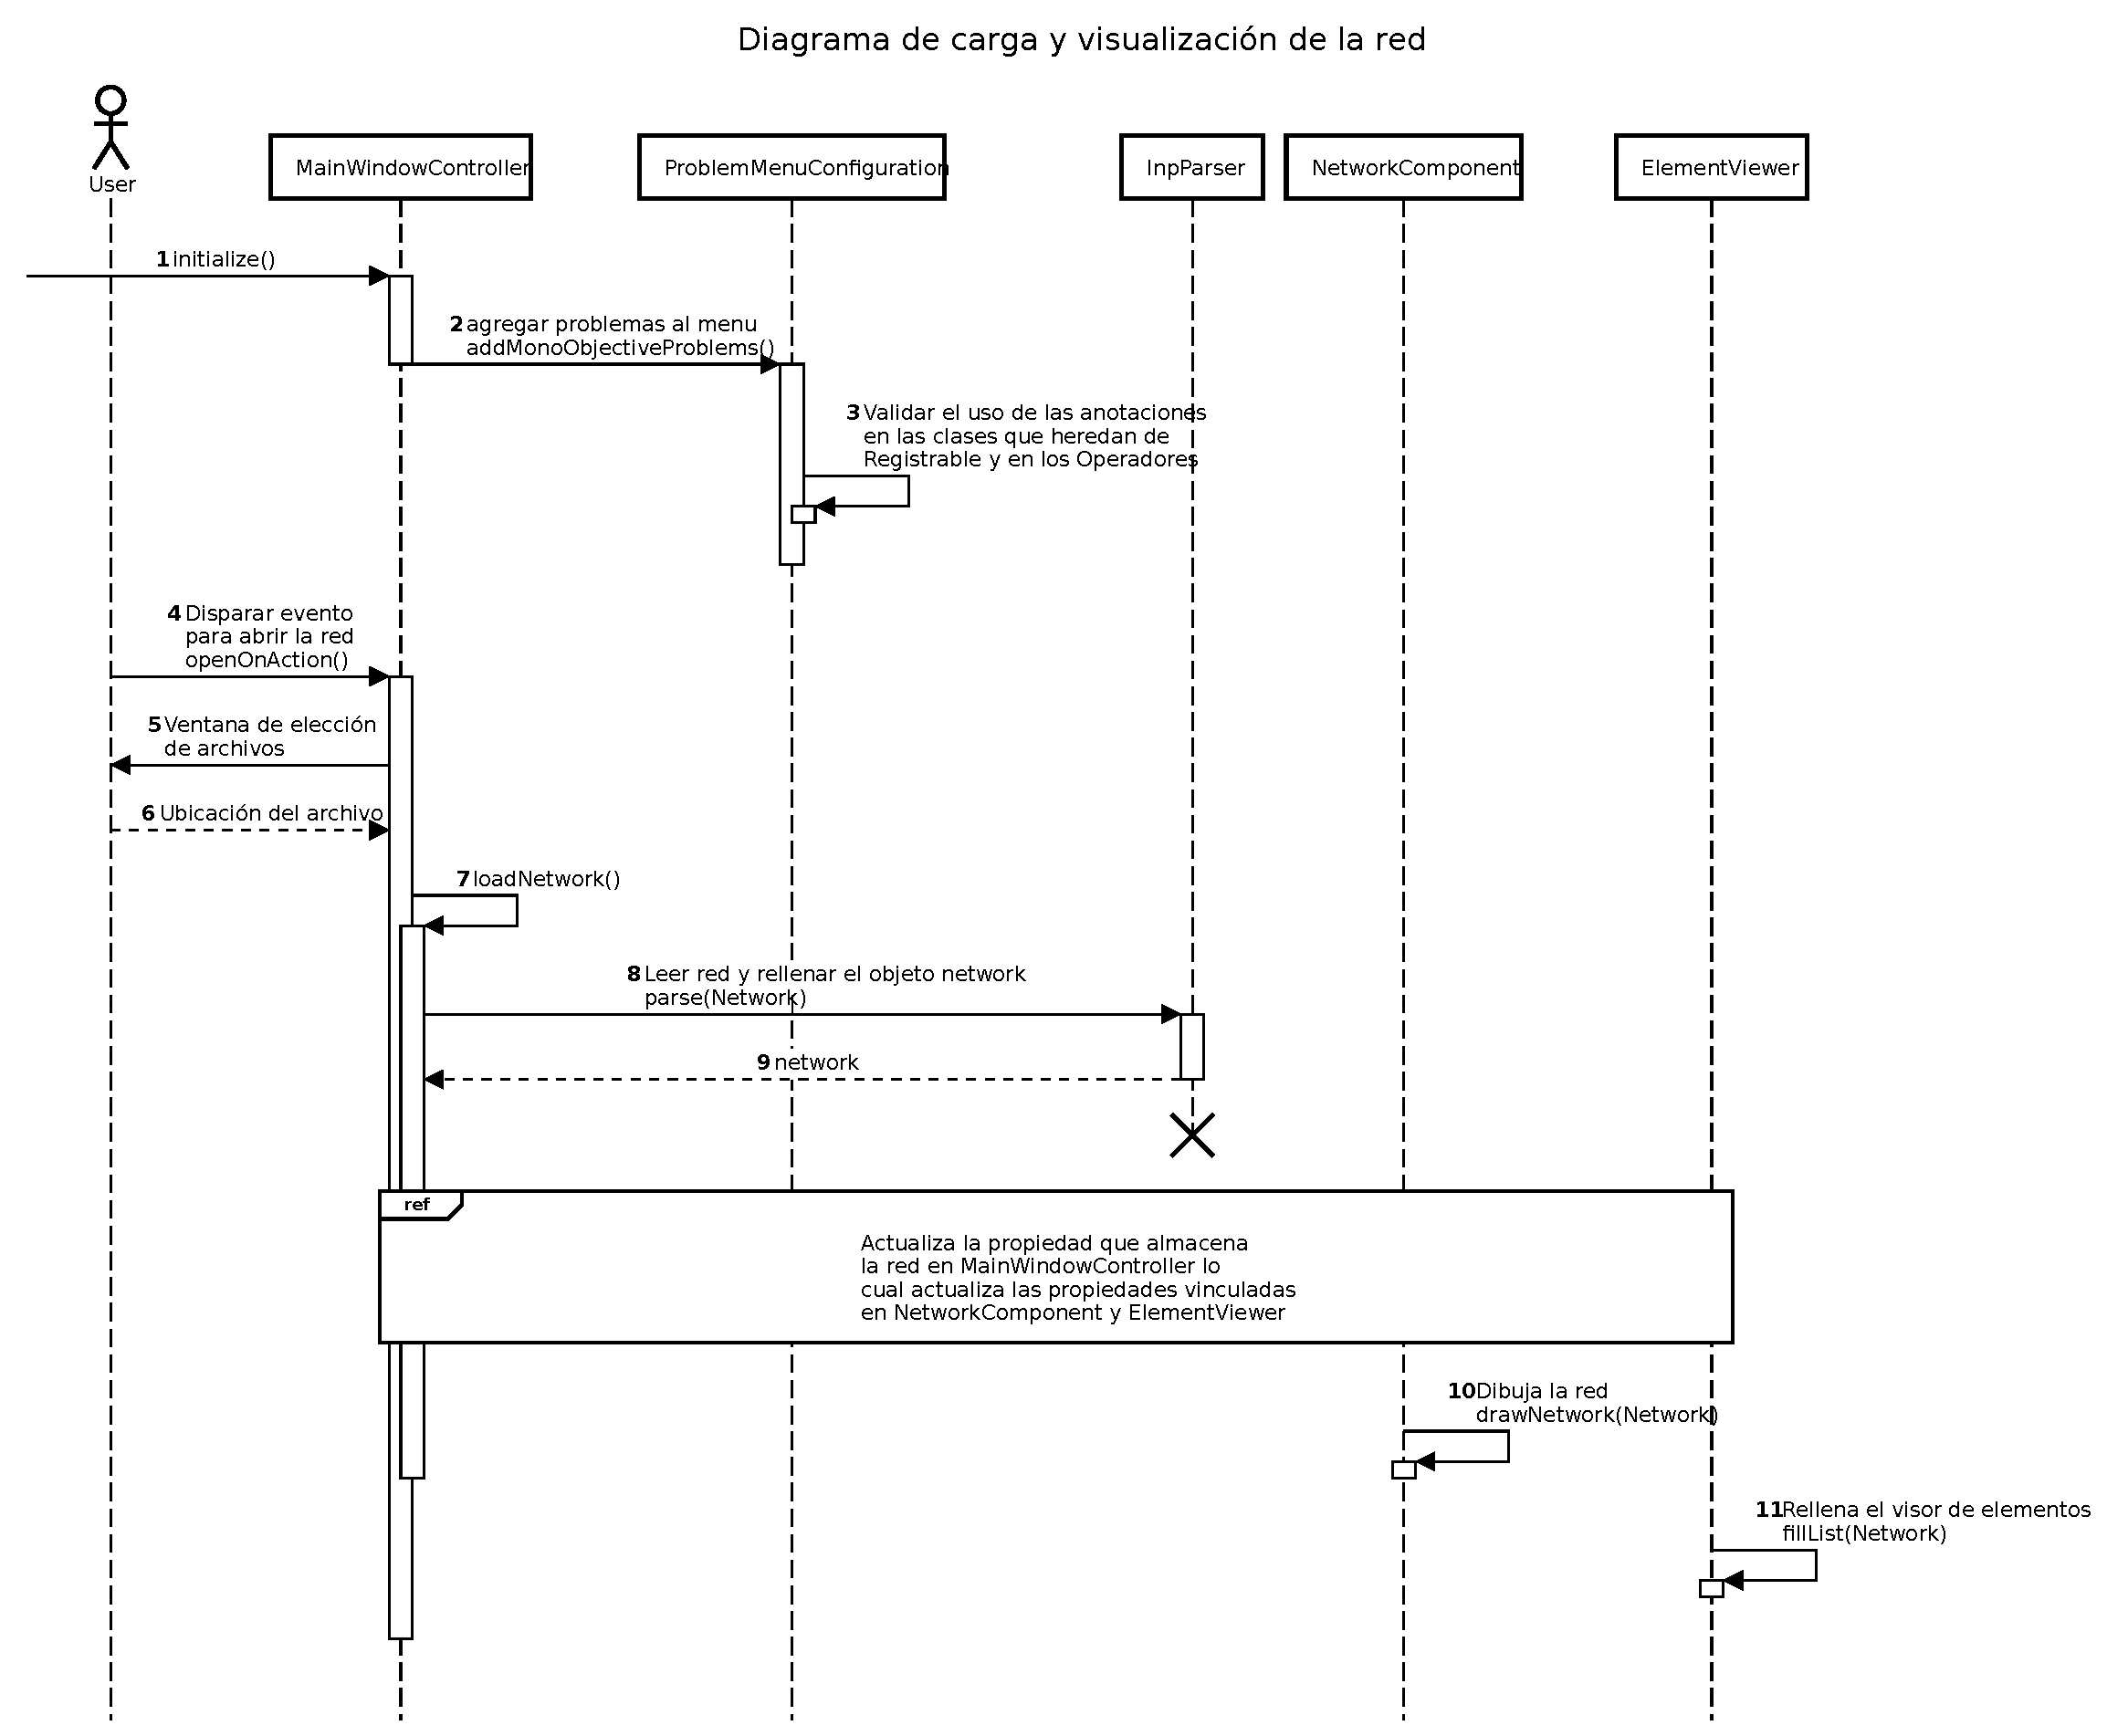
\includegraphics[height=\textwidth, angle=90]{Capitulo4/assets/d_sec_visualizacion.eps}
  \caption{Diagrama de secuencia de la carga y visualizaci�n de la red}
  \label{fig:dia_sec_visualizacion}
\end{figure}

\paragraph{Funcionalidad 2:} Esta es una de las funcionalidades ligada al modulo metaheur�stica y debido a uno de los requisitos establecidos por el cliente de que la aplicaci�n debe poder extender el n�mero de algoritmos, operadores y problemas implementados es necesario implementar una jerarqu�a de clases que facilite lo anteriormente mencionado. Es por ello, que se utilizo como base la jerarqu�a de clases utilizada por el Framework JMetal~\cite{Durillo2010} la cual fue adaptada para ser ocupada por esta aplicaci�n. La Figura~\ref{fig:dia_class_met} corresponde a la jerarqu�a ya mencionada.


\begin{figure}[h]
  \centering
  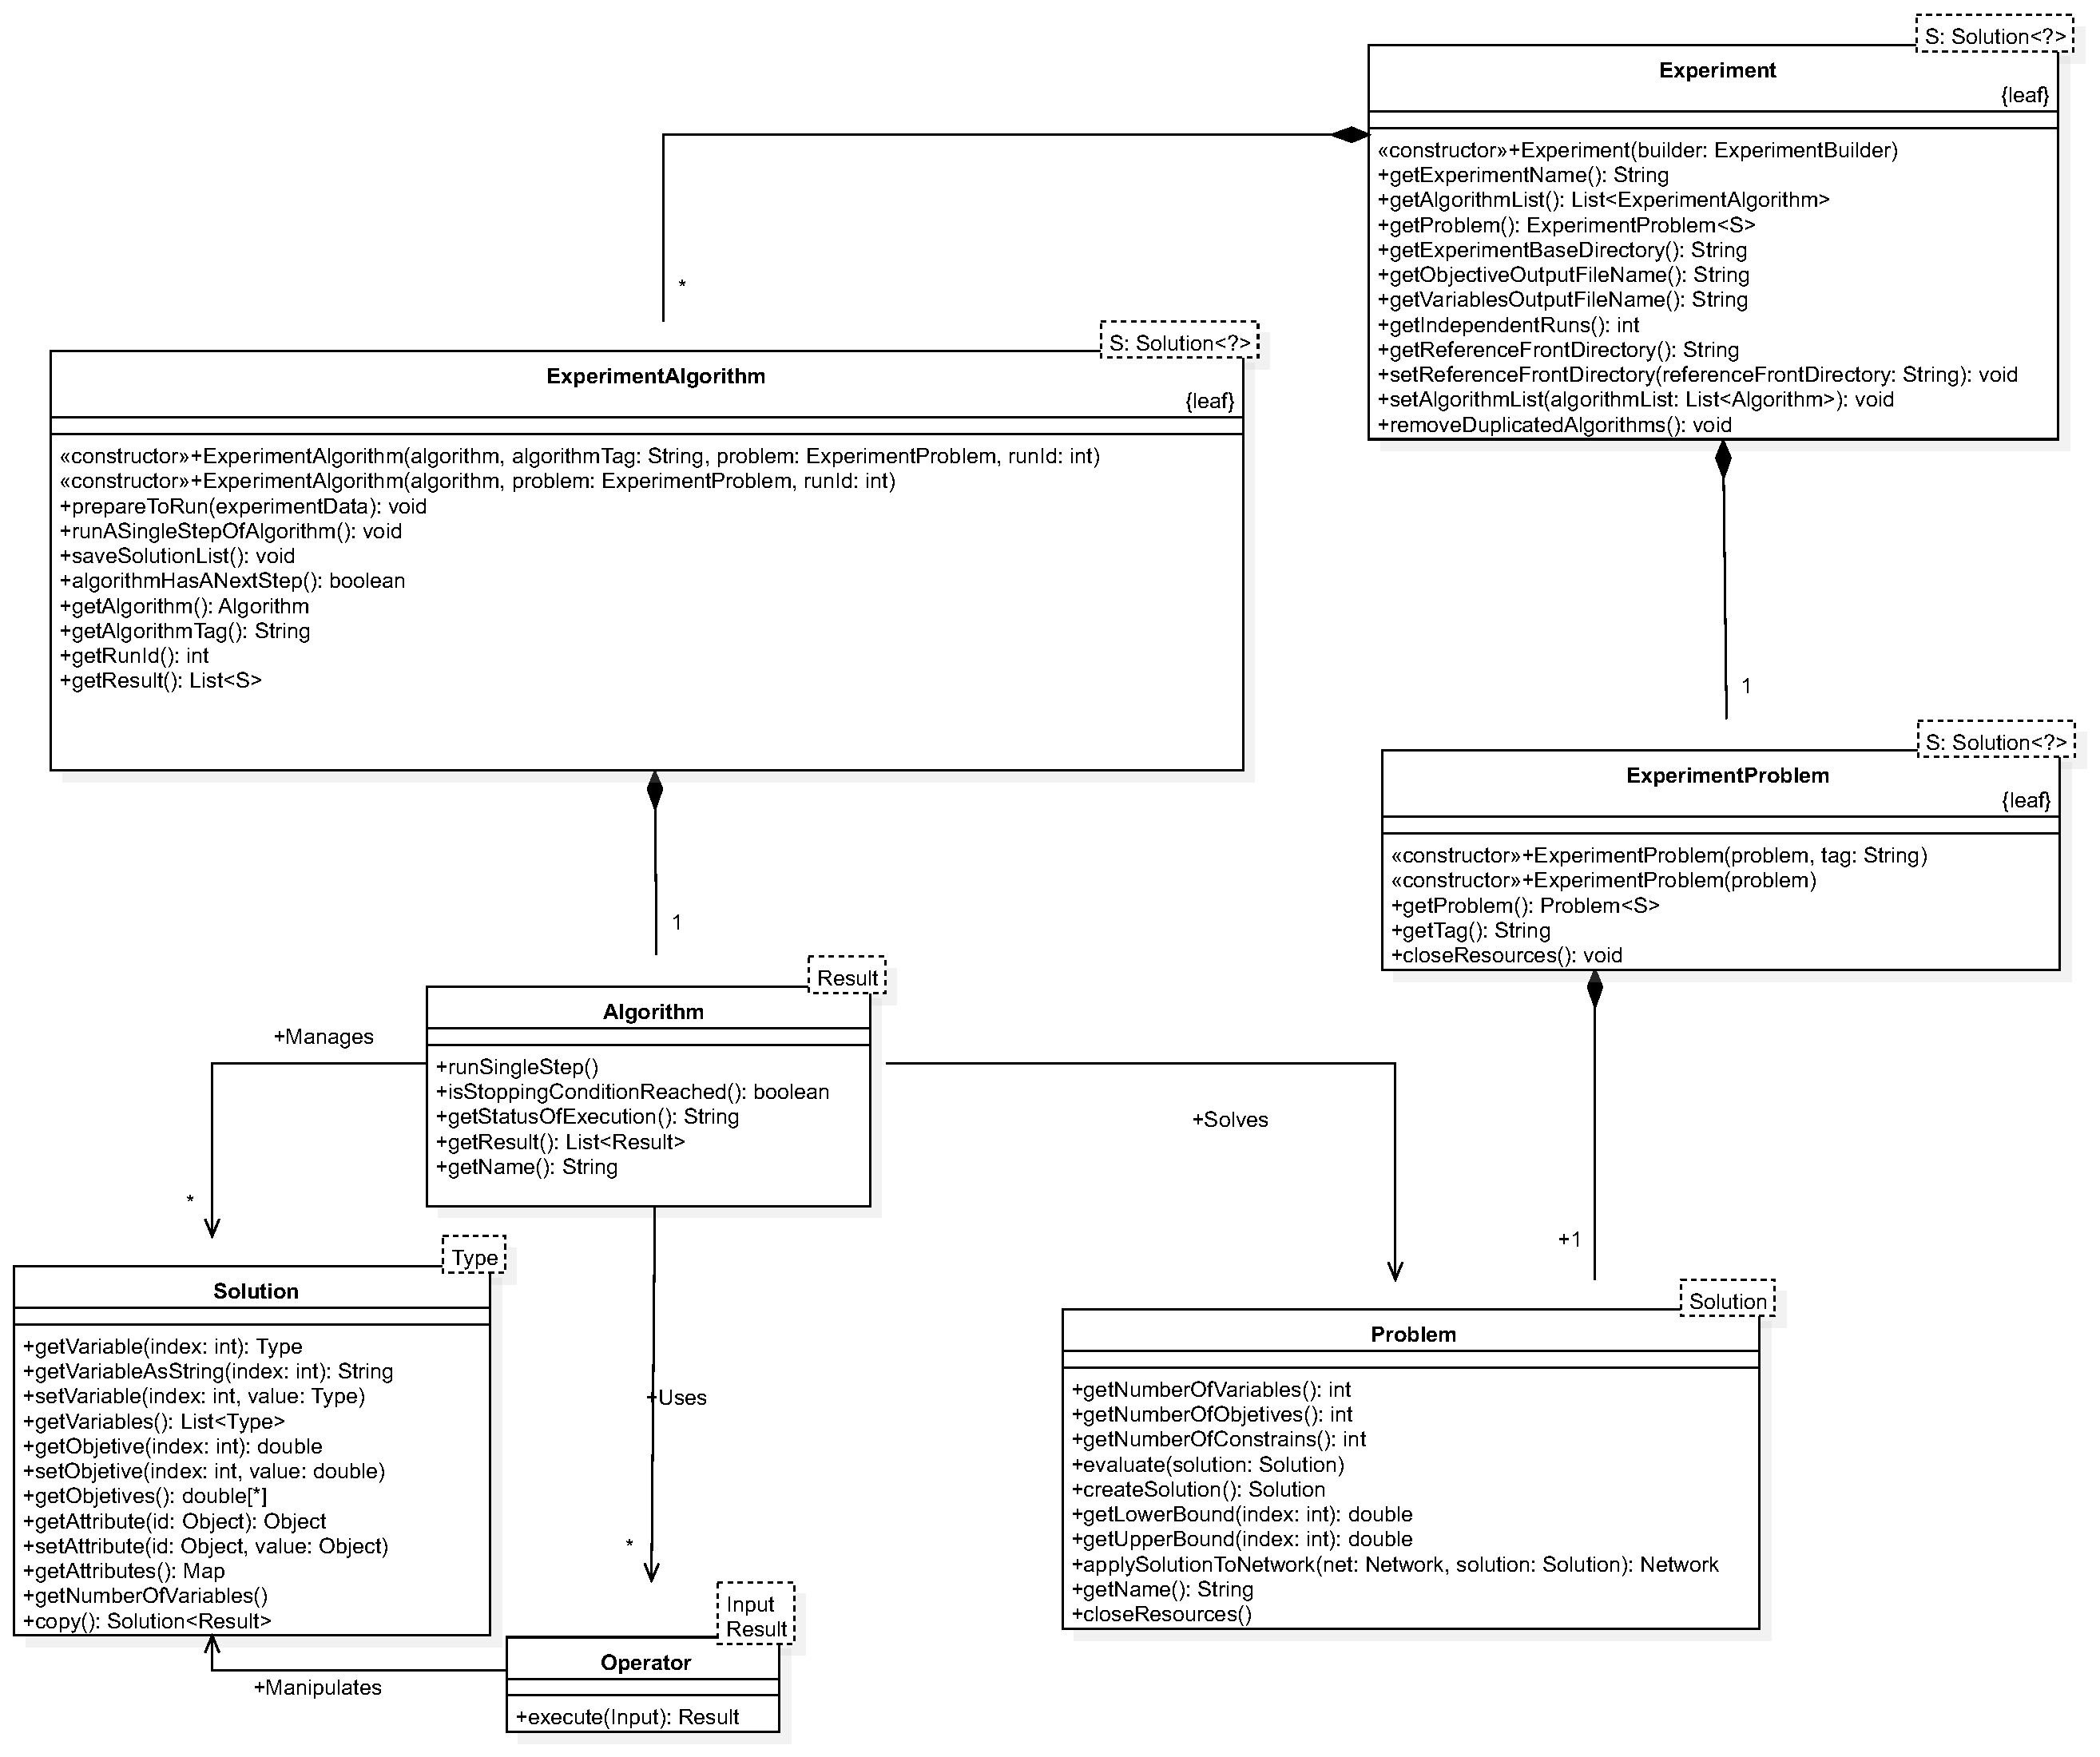
\includegraphics[height=\textwidth, angle=90]{Capitulo4/assets/d_clases_metaheuristica.eps}
  \caption{Diagrama de clases modulo metaheur�stica. Modificaci�n a partir del diagrama presentado en~\cite{Durillo2010}}
  \label{fig:dia_class_met}
\end{figure}

%%%%%%%%%%%%%%%%%%%%%%%%%%%%%%%

Debido a la importancia que tienen las metaheur�sticas para la aplicaci�n, se explicar� de manera general que realiza cada una de las clases e interfaces presentes en la Figura~\ref{fig:dia_class_met}.

\textit{\textbf{Algorithm}} es la interfaz desde la que se heredan, ya sea directa o indirectamente, cada uno de los algoritmos metaheur�sticos implementados por la aplicaci�n. Su principal m�todo es \textit{runASingleStep} puesto que �ste permite realiza una �nica iteraci�n del algoritmo, permitiendo as� que el programa interactu� con la instancia del algoritmo. Esta interacci�n permite recuperar los resultados intermedios de la optimizaci�n, as� como tambi�n cancelar la ejecuci�n. Un ejemplo de la implementaci�n de este m�todo para GA se muestra en la Figura~\ref{fig:runSingleStep}.

\begin{figure}[h]
  \begin{lstlisting}
int step = 0;
List<IntegerSolution> population;
public void runSingleStep() throws Exception, EpanetException {
  List<S> offspringPopulation;
  List<S> selectionPopulation;

  // Durante la primera iteraci�n inicializa 
  // y eval�a la poblaci�n
  if (step == 0) {
    population = createInitialPopulation();
    population = evaluatePopulation(population);
    initProgress();
  }
  // Desde la segunda iteraci�n en adelante selecciona
  // y reproduce las soluciones
  if (!isStoppingConditionReached()) {
    selectionPopulation = selection(population);
    offspringPopulation = reproduction(selectionPopulation);
    offspringPopulation = evaluatePopulation(offspringPopulation);
    population = replacement(population, offspringPopulation);
    updateProgress();
  }

  this.step++;
}
  \end{lstlisting}
  \caption{C�digo del m�todo \textit{runSingleStep} utilizado con GA y NSGAII}
  \label{fig:runSingleStep}
\end{figure}

\textit{\textbf{Solution}} es la interfaz que representa la soluci�n del problema. La aplicaci�n implementa esta interfaz en una clase llamada \textit{IntegerSolution}, la cual permite trabajar variables de decisi�n de tipo entero.

\textit{\textbf{Operator}} es la interfaz de la que heredan todos los tipos de operadores usado en la aplicaci�n. Los operadores son clases que contienen una funci�n que trabaja sobre una o un conjunto de soluciones. Sus usos son muy variables, entre ellos se encuentra la selecci�n de soluciones dentro de un conjunto, la modificaci�n de las variables de decisi�n de una soluci�n y la combinaci�n de dos soluciones con el fin de generar unas nuevas.

\textit{\textbf{Problem}} es la interfaz de la que heredan todos los problemas. Las clases que implementan esta interfaz son las que se encargan de evaluar y penalizar las soluciones generadas por los algoritmos metaheur�sticos en el m�todo \textit{evaluate}. Adicionalmente, esta clase es usada para mapear una soluci�n sobre la red cargada y de esta manera poder generar un nuevo archivo de configuraci�n de red. El m�todo que realiza esto ultimo es \textit{applySolutionToNetwork}.

Las clases \textit{\textbf{ExperimentAlgorithm}} y \textit{\textbf{ExperimentProblem}} act�an como envoltorios para las clases \textit{Algorithm} y \textit{Problem} incorporando algunas funciones adicionales.

Por ultimo la clase \textit{\textbf{Experiment}} es un contenedor de algoritmos. Cada algoritmo agregado al experimento corresponde a una iteraci�n independiente. Actualmente, se pensaron los experimentos para solo contener varias instancias de un mismo algoritmo. Los algoritmos deben ser acoplados a un \textit{ExperimentAlgorithm} antes de ser agregados al Experimento.

Cada una de las clases explicadas anteriormente tiene un bajo acoplamiento entre ellas, as� como del resto de la aplicaci�n puesto que se hace uso de la t�cnica llamada Polimorfismo. Esto permite combinar cada una de ellas de diferentes maneras, por ejemplo, se pueden usar distintos algoritmos para el mismo tipo de problema. La limitaci�n de esto es que el problema debe ser compatible con el algoritmo, es decir, si el algoritmo esta dise�ado para ser monoobjetivo, entonces el problema debe tener un solo objetivo.
%%%%%%%%%%%%%%%%%%%%%%%%%%%%%%%

El diagrama de secuencia de la Figura~\ref{fig:dia_sec_opt} muestra la interacci�n de las clases con del modulo metaheur�sticas, con el resto de clases de la aplicaci�n.


\begin{figure}[h]
  \centering
  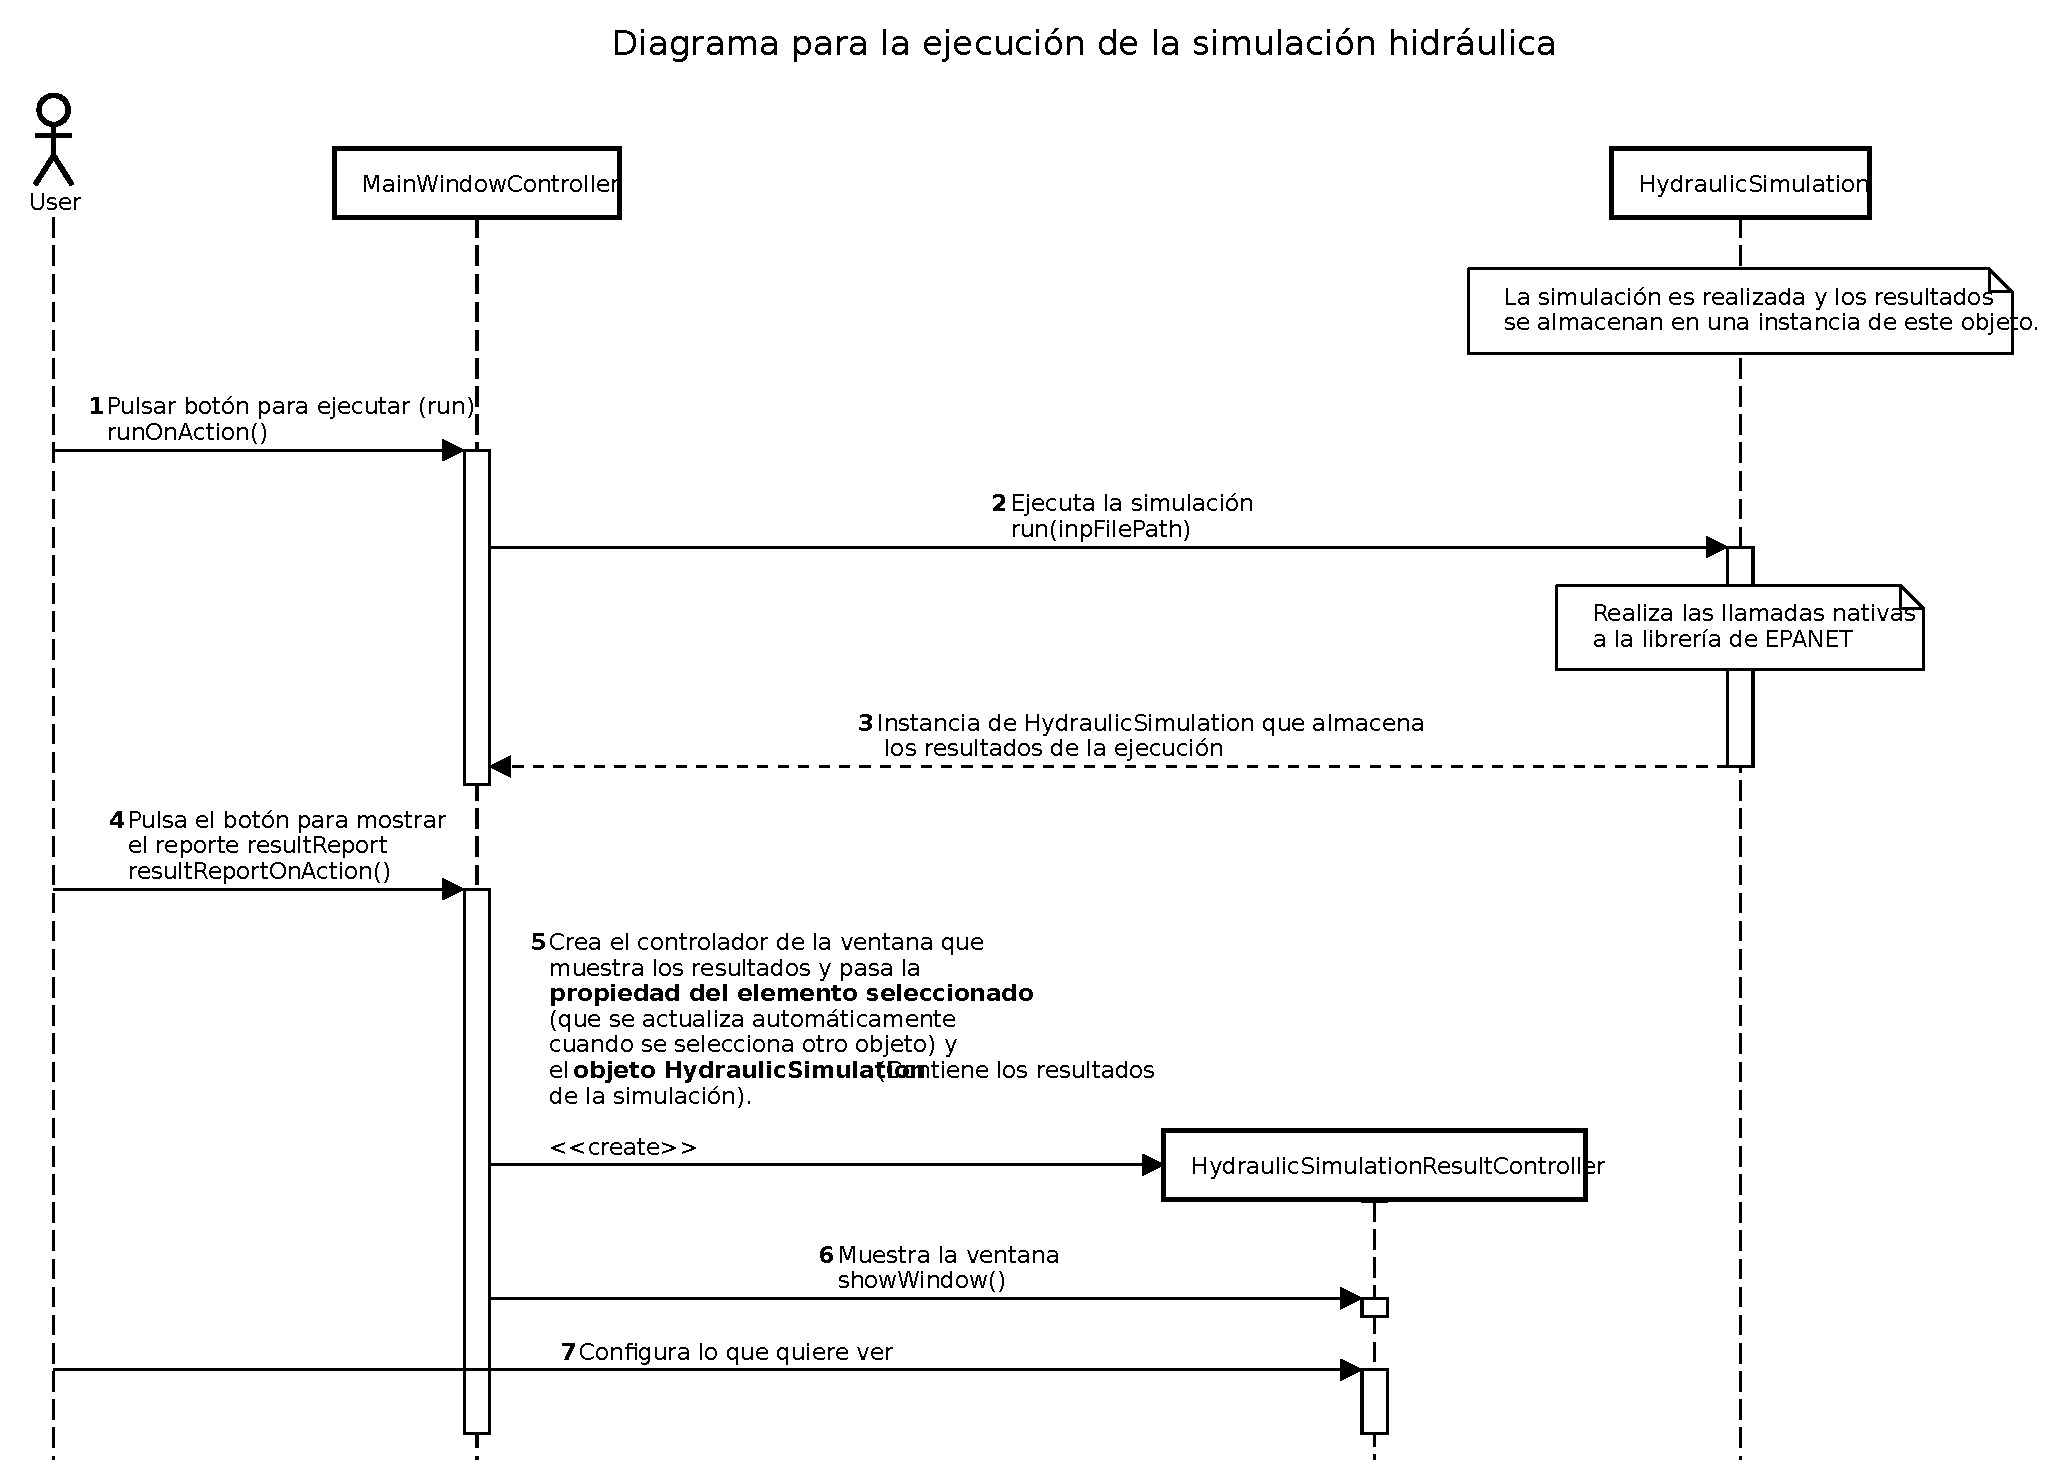
\includegraphics[width=\textwidth]{Capitulo4/assets/d_seq_simulacion-monomulti.eps}
  \caption{Diagrama de secuencia para llevar a cabo la optimizacion de los problemas}
  \label{fig:dia_sec_opt}
\end{figure}

\paragraph{Funcionalidad 3:} Para implementar esta funcionalidad es necesario implementar un conjunto de clases las cuales guardar�n los resultados de la simulaci�n para cada uno de los nodos y enlaces de una red. Estas nuevas clases son las mostradas en la Figura~\ref{fig:dia_class_sim_hyd}.


\begin{figure}[h]
  \centering
  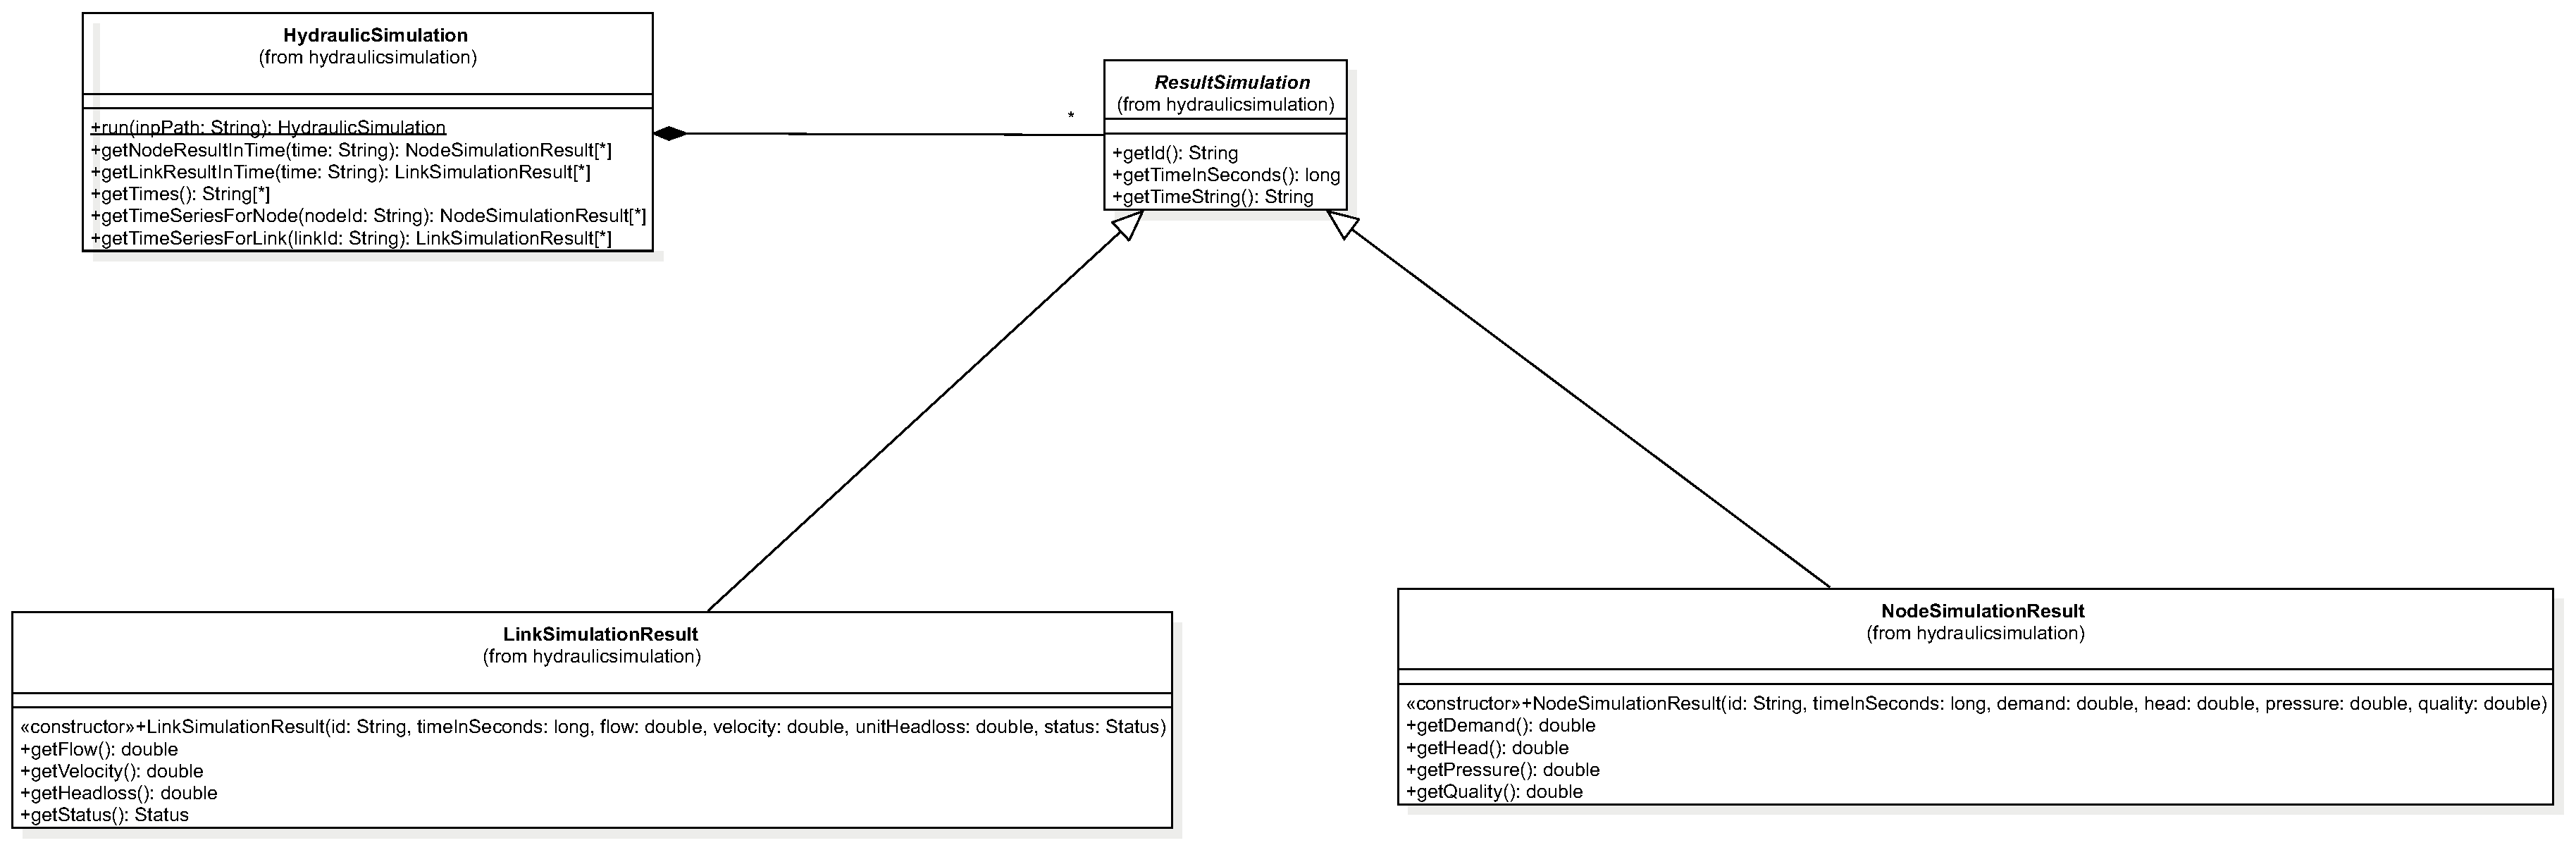
\includegraphics[width=\textwidth]{Capitulo4/assets/d_clases_hyd_simulation.eps}
  \caption{Diagrama de clases para la simulaci�n hidr�ulica}
  \label{fig:dia_class_sim_hyd}
\end{figure}

El diagrama de secuencia presentado en la Figura~\ref{fig:dia_sec_sim_hyd} muestra la interacci�n entre las clases necesarias para realizar la simulaci�n hidr�ulica utilizando los valores del archivo de red cargado.

\begin{figure}[h]
  \centering
  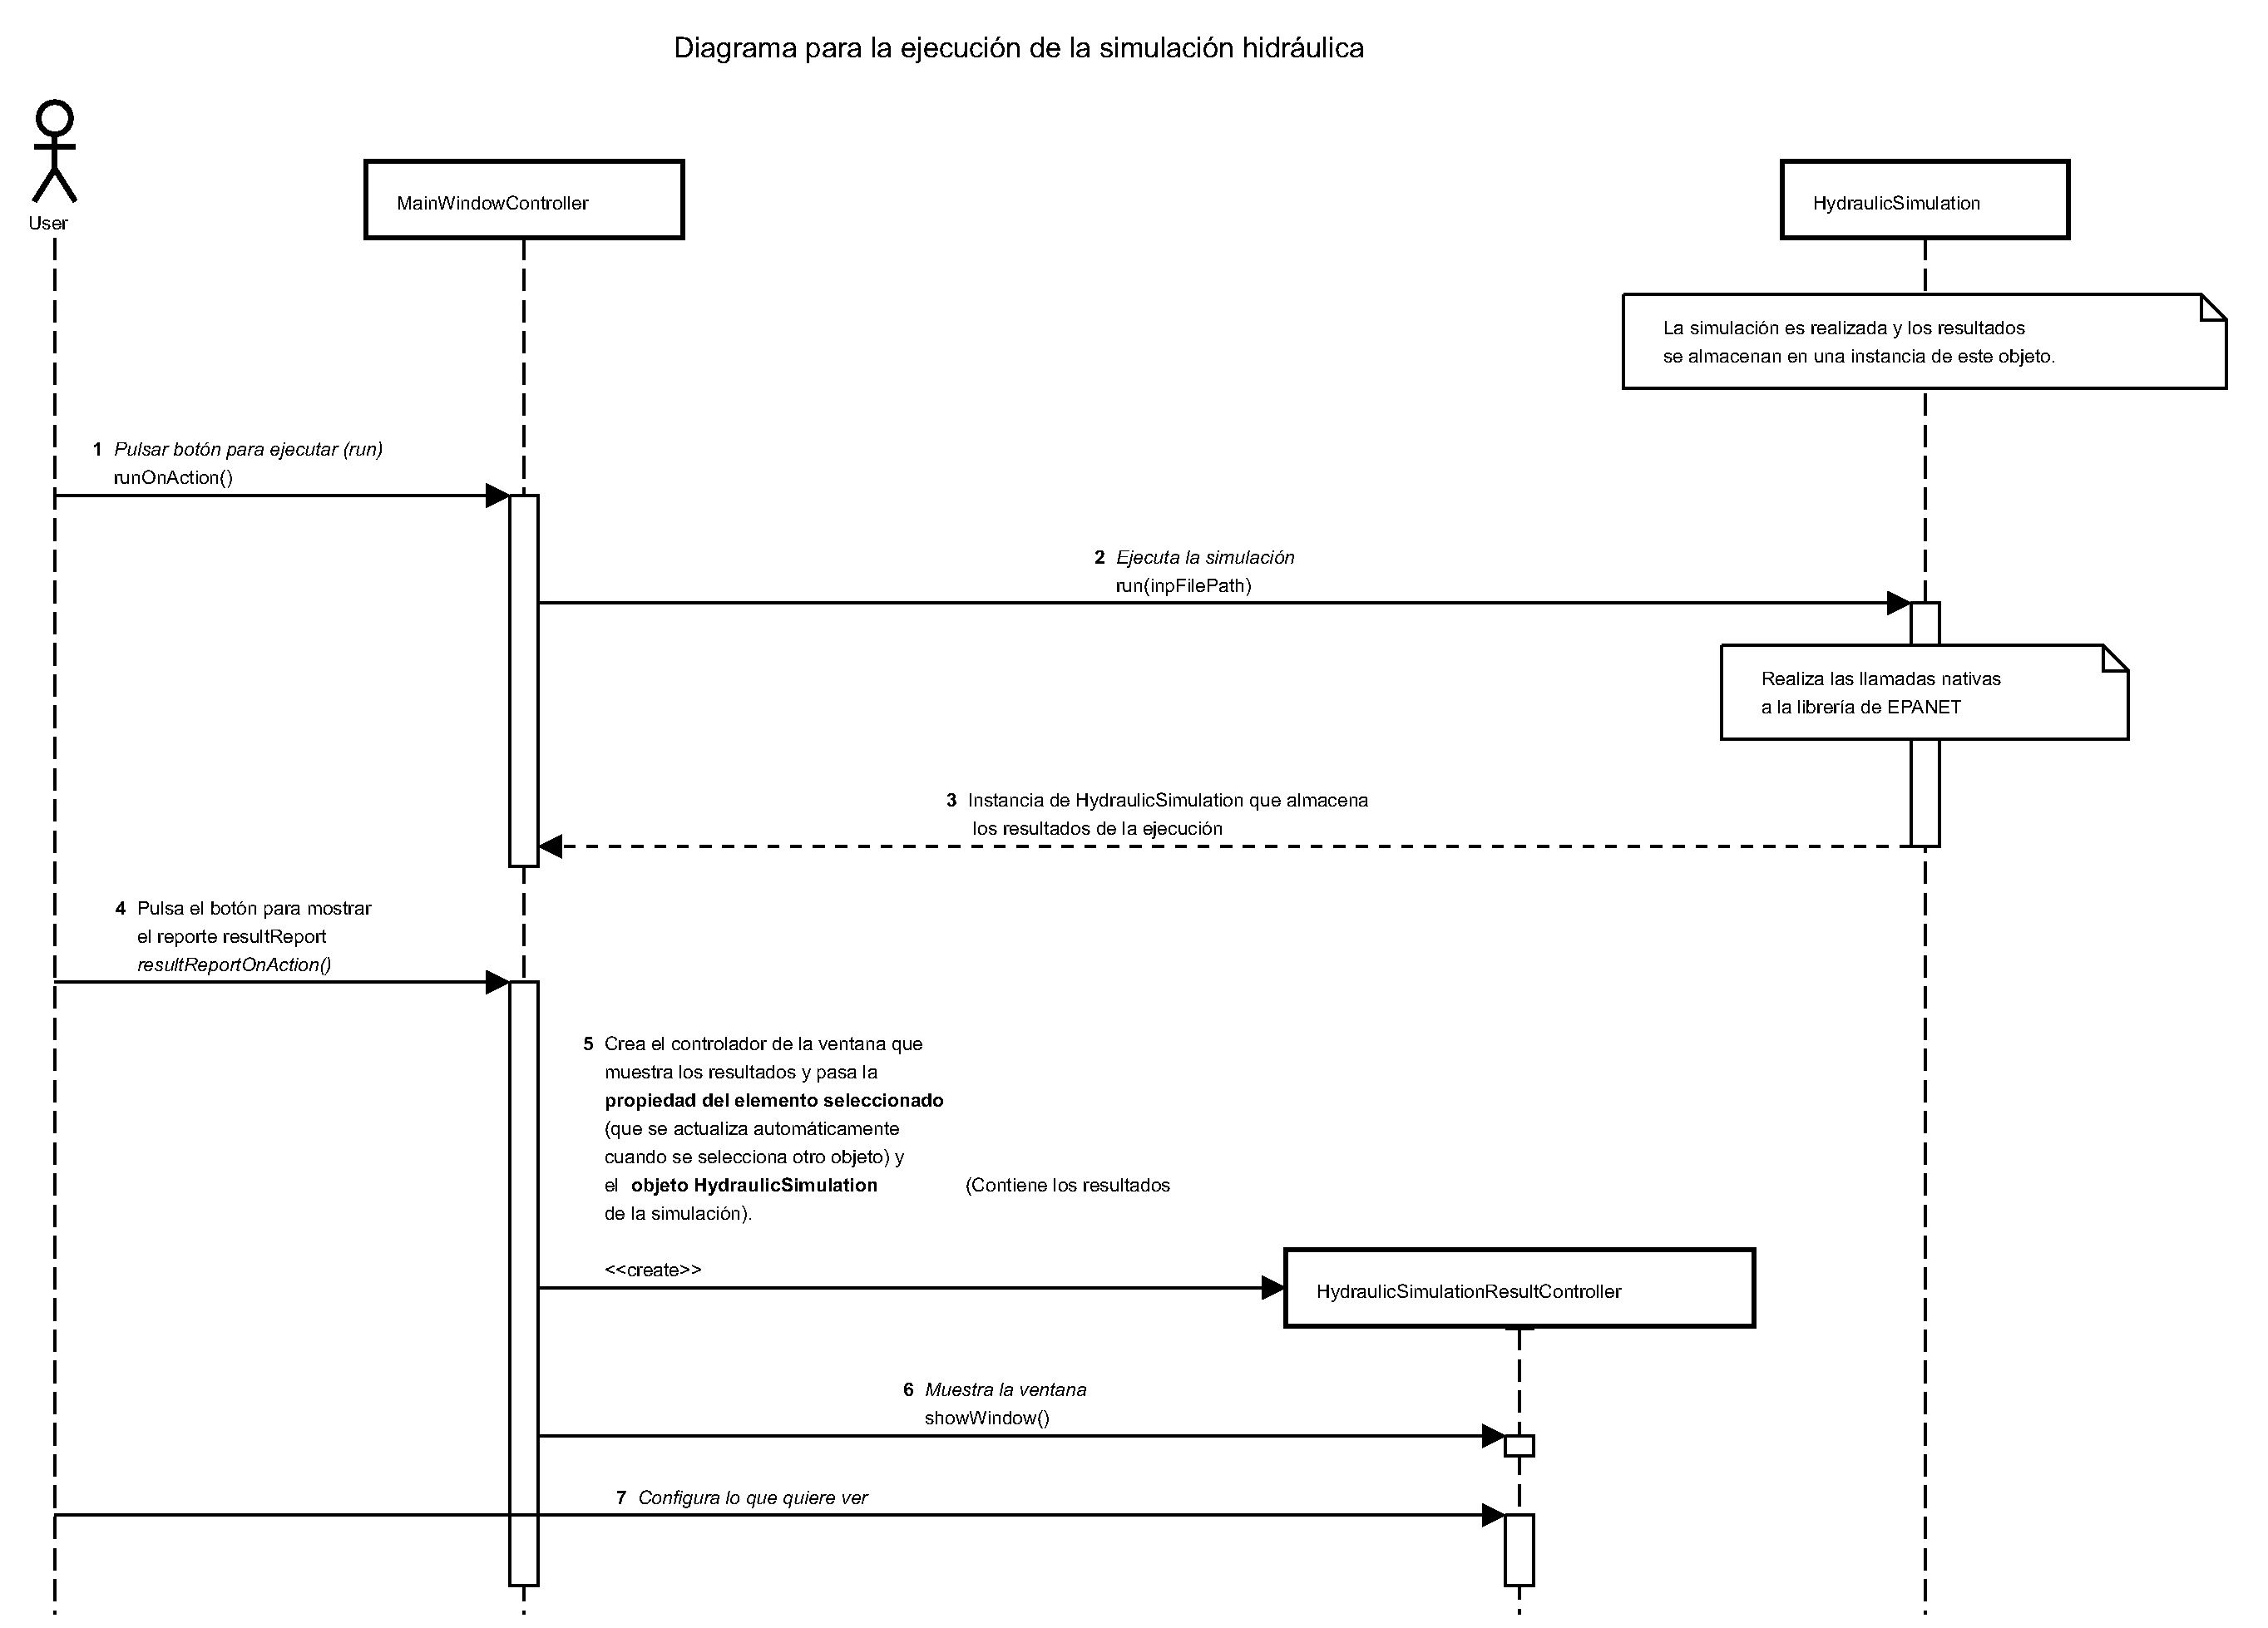
\includegraphics[height=\textwidth, angle=90]{Capitulo4/assets/d_seq_simulacion-hidraulica.eps}
  \caption{Diagrama de secuencia para realizar la simulaci�n hidr�ulica}
  \label{fig:dia_sec_sim_hyd}
\end{figure}


%% Extensibilidad
En diferentes secciones de este documento se ha mencionado que la aplicaci�n debe ser extensible, refiri�ndonos al hecho de que se deben poder agregar nuevos algoritmos, operadores y problemas. Una vez alcanzada la tercera iteraci�n fue necesario hacer frente a este problema. Sin embargo, �ste no es un problema f�cil de abordar. Las ideas que surgieron para tratar este problema eran diversas. Una de ellas, por ejemplo, consist�a en que el usuario implementara por si mismo la interfaz de configuraci�n de los nuevos problemas y algoritmos que ha a�adido, asi como que se encargue de que estas ventanas fueran visibles desde la aplicaci�n. No obstante, realizar �sta tarea consist�a en que se deb�a tener conocimiento de la implementaci�n de interfaces gr�ficas usando JavaFX.
  
Finalmente se decidi� utilizar un enfoque parecido al de los Frameworks como Spring y JUnit. Para esto se creo la jerarqu�a de clases que se muestra en la Figura~\ref{fig:registrable}. Esta jerarqu�a define la interfaz \textit{Registrable} y dos subinterfaces extras que son \textit{SingleObjectiveRegistrable} y \textit{MultiObjectiveRegistrable}. \textit{SingleObjectiveRegistrable} debe ser usada cuando el nuevo problema es del tipo monoobjetivo, mientras que \textit{MultiObjectiveRegistrable} cuando el problema es multiobjetivo.

% Esta clase actu� como una plantilla para crear nuevos experimentos. Junto con esta jerarqu�a se definieron un conjunto de anotaciones que son le�das durante la ejecuci�n del problema al querer optimizar una red y son utilizadas para construir la interfaz gr�fica y posteriormente inyectar en el constructor de la clase al crear la instancia las configuraciones y operadores a utilizar para la optimizaci�n.

% que Esto es, crear anotaciones que puedan ser le�das en tiempo de ejecuci�n por el programa. Las anotaciones creadas permiten indicar los valores que se pueden configurar del problema, asi como los operadores a ser utilizados por un algoritmo. Las anotaciones son le�das desde el programa al momento de querer optimizar una RDA, permitiendo de esa manera construir dinamicamente una interfaz de usuario para configurar los detalles del algoritmo, operador y el problema a resolver. Finalmente, una vez configurados todos los detalles anteriormente mencionados, haciendo uso de \textit{Java Reflection} se crea una nueva instancia.

% , adem�s de la modularidad proporcionada descrita por el diagrama de clases de la Figura \ref{fig:dia_class_met}, presentado para la Funcionalidad 2, se hace uso de una interfaz desde la cual se permiten definir plantillas para crear nuevos experimentos y acoplarlos a la aplicaci�n. Dicha interfaz se muestra en la Figura~\ref{fig:registrable}.

\begin{figure}[h]
    \centering
    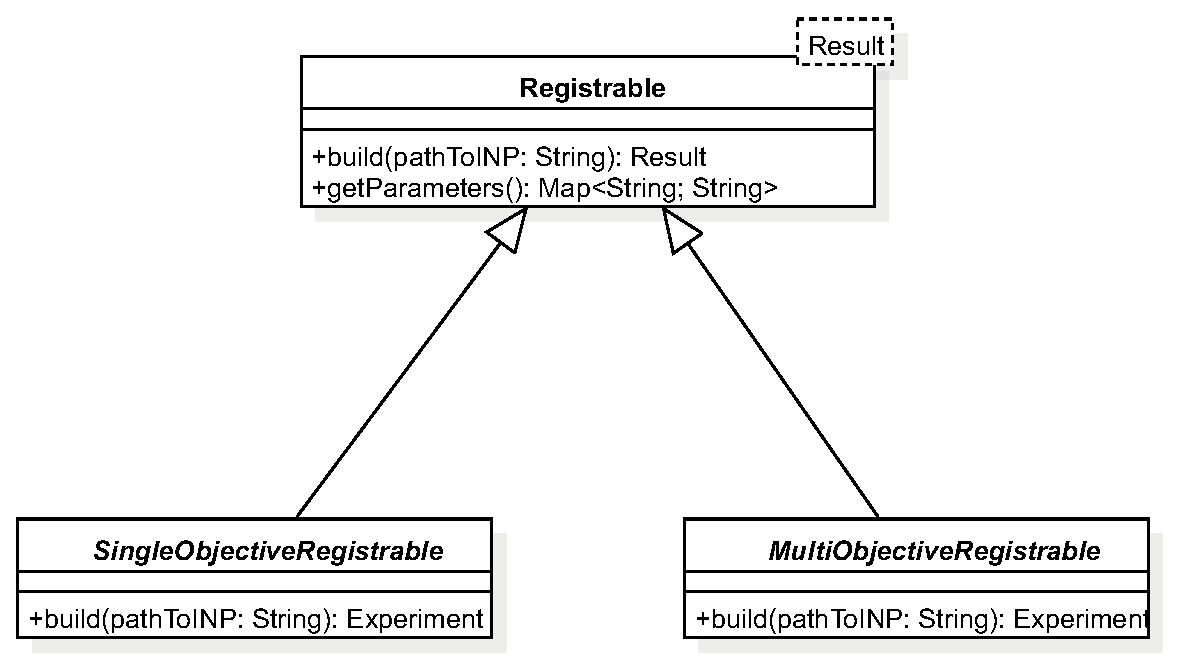
\includegraphics[width=\textwidth]{Capitulo4/assets/d_class_registrable.eps}
    \caption{Interfaz de clase \textit{Registrable}.}
    \label{fig:registrable}
\end{figure}

En el \textbf{Anexo~\ref{appendix:diseno}} se puede ver la el documento de dise�o de la aplicaci�n.

\clearpage

\section{Implementaci�n}
Con la fase de dise�o finalizada, se procede a realizar la fase de implementaci�n. Durante esta fase se genera el c�digo de la aplicaci�n y se genera el manual de usuario.

La aplicaci�n fue desarrollada en el lenguaje Java version 1.8. Con el fin de crear las interfaces de usuario se utilizo el Framework JavaFX.

En el cuadro~\ref{fig:actualizacion_implementacion} se presenta las tareas realizadas durante esta fase del desarrollo del software.

\begin{longtable}{||c| m{10cm}||}
  \caption{Actividades fase de implementaci�n}
  \label{fig:actualizacion_implementacion}
  \endfirsthead
  \hline
  N� Iteraci�n & Descripci�n\\ [0.5ex] 
  \hline\hline
  1 & Se codifican las clases para cargar la red \textit{Network}.\\
  \hline
  2 & Se codifican las clases del modulo metaheuristica. \newline Se implementa el Algoritmo Gen�tico.\newline Se implementa la codificaci�n del problema monoobjetivo \textit{Pipe Optimizing}. \newline Se implementan los operadores IntegerRandomMutation, SBXCrossover, IntegerPolinomialMutation, IntegerRangeRandomMutation y UniformSelection.\\
  \hline
  3 & Se implementan la interfaz de usuario principal. \newline Se implementa el componente para visualizar la red \newline Se implementa la interfaz de configuraci�n del problema. \newline Se implementa la interfaz de visualizaci�n de resultados de optimizaci�n. \newline Se implementa la interfaz que muestra el gr�fico con los resultados de la optimizacion. \newline Se implementa la funcionalidad para guardar las soluciones en TSV. \newline Se implementa funcionalidad para exportar la soluci�n escogida como un inp(Formato del archivo de configuraci�n de red). \\
  \hline
  4 & Se agrega el algoritmo NSGAII. \newline Se implementa la codificaci�n del problema multiobjetivo \textbf{Pumping Schedule}.\\
  \hline
  5 & Se modifican las clases y archivos relacionados a la interfaces de usuario. \newline Se implementa la funcionalidad para realizar m�ltiples simulaciones independientes de un mismo algoritmo para los problemas multiobjetivos (Experimentos). \newline Se implementa la funcionalidad para realizar la simulaci�n usando los valores del archivo de red.\\
  \hline
  6 & Se modifica el componente de visualizaci�n de red para mostrar para cada tipo de elemento que conforma la red un s�mbolo distinto. \newline Se implementa funcionalidad para mostrar una leyenda de los s�mbolos. \newline Se implementa ventana de configuraci�n de la aplicaci�n. \newline Se implementa la funcionalidad para realizar m�ltiples simulaciones independientes para los problemas monoobjetivo (Se adapta para utilizar los Experimentos antes utilizados solo en problemas multiobjetivos).\newline Se permite agregar valores por defecto en la ventana de configuraci�n del problemas. \newline Se implementa la funcionalidad para exportar resultados a un Excel.\\
  \hline
\end{longtable}

A continuaci�n se presentara para cada una de las funcionalidades escogidas las interfaces implementadas.

\paragraph{Funcionalidad 1}: La Figura~\ref{fig:ventana_visualizacion} muestra la ventana de visualizaci�n de la red.

\begin{figure}[H]
  \centering
  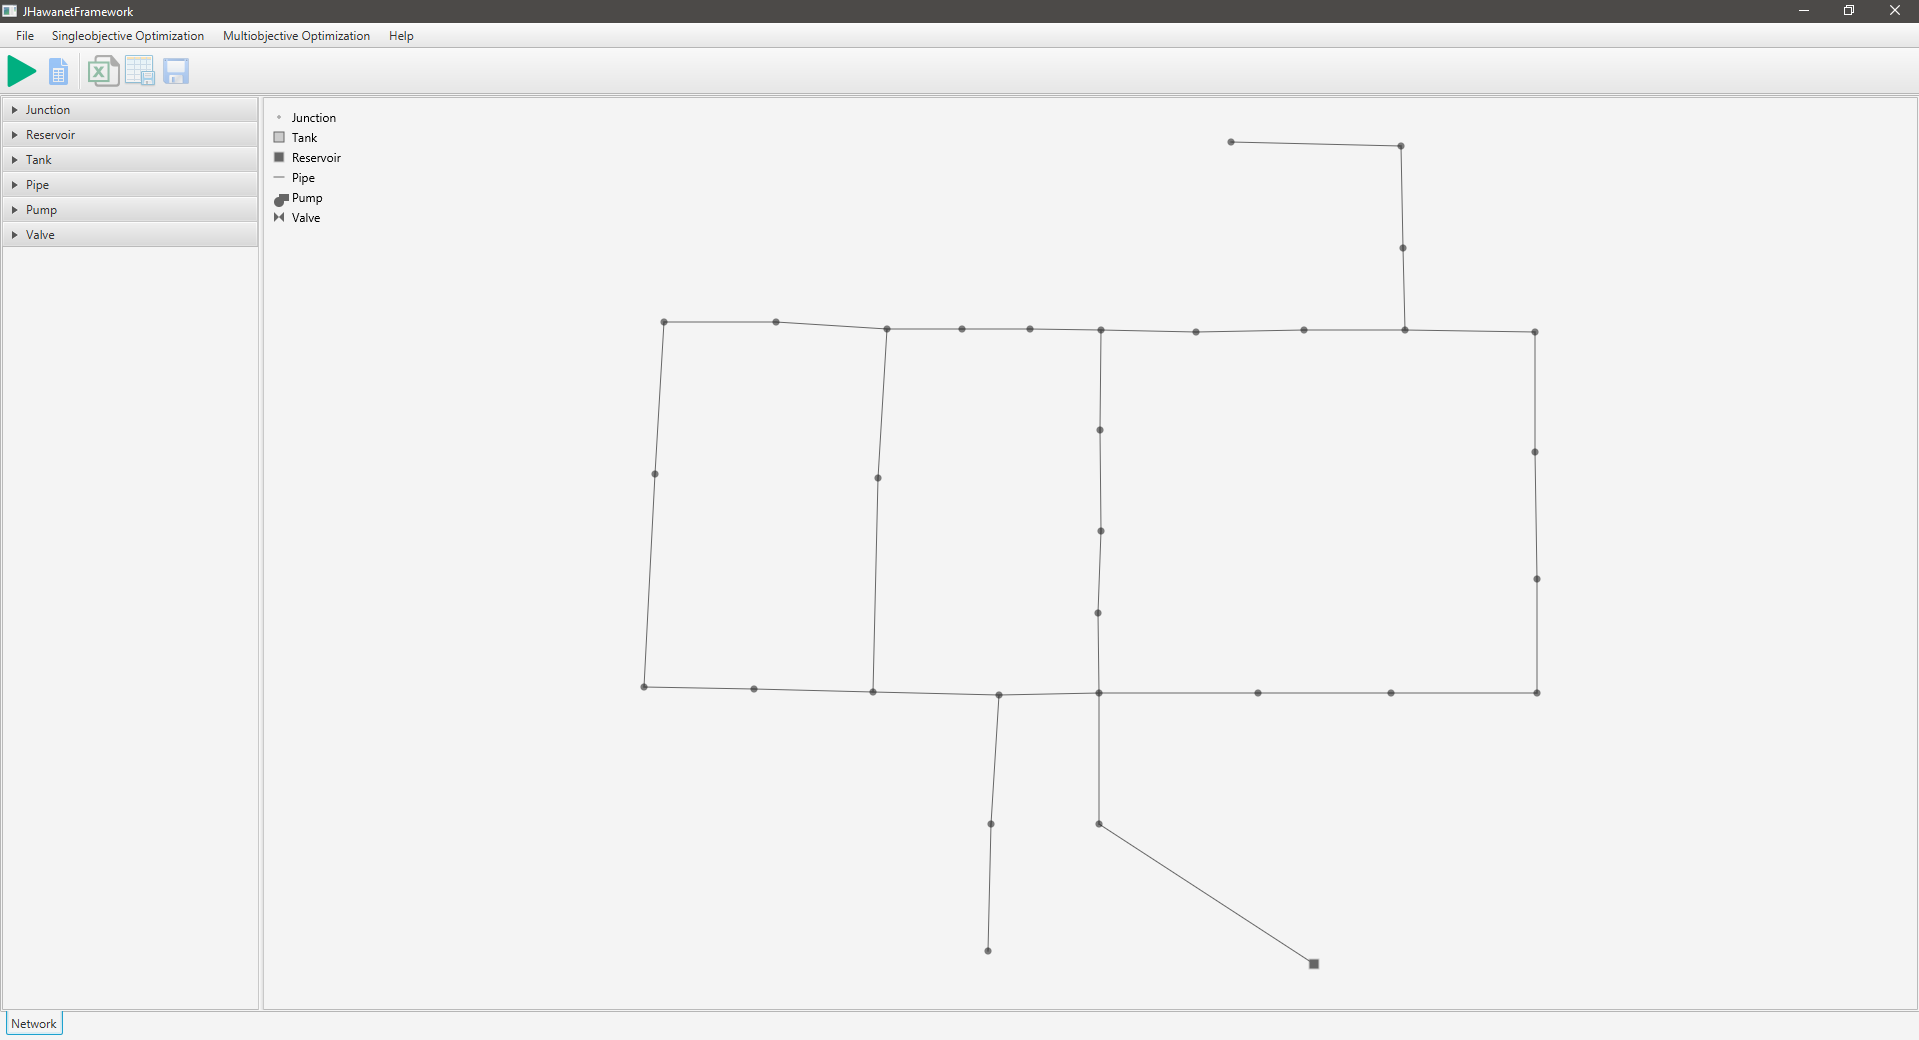
\includegraphics[width=\textwidth]{Capitulo4/assets/VisualizacionRed.png}
	\caption{Ventana principal de la aplicaci�n donde se visualiza la red}
	\label{fig:ventana_visualizacion}
\end{figure}

\paragraph{Funcionalidad 2}: Las Figuras~\ref{fig:ventana_descripcion},~\ref{fig:ventana_configuracion_problema},~\ref{fig:ventana_operador},~\ref{fig:ventana_retroalimentacion} y~\ref{fig:ventana_resultados_opt} muestran las ventana utilizadas durante el cumplimiento de esta funcionalidad.

\begin{figure}[H]
  \centering
  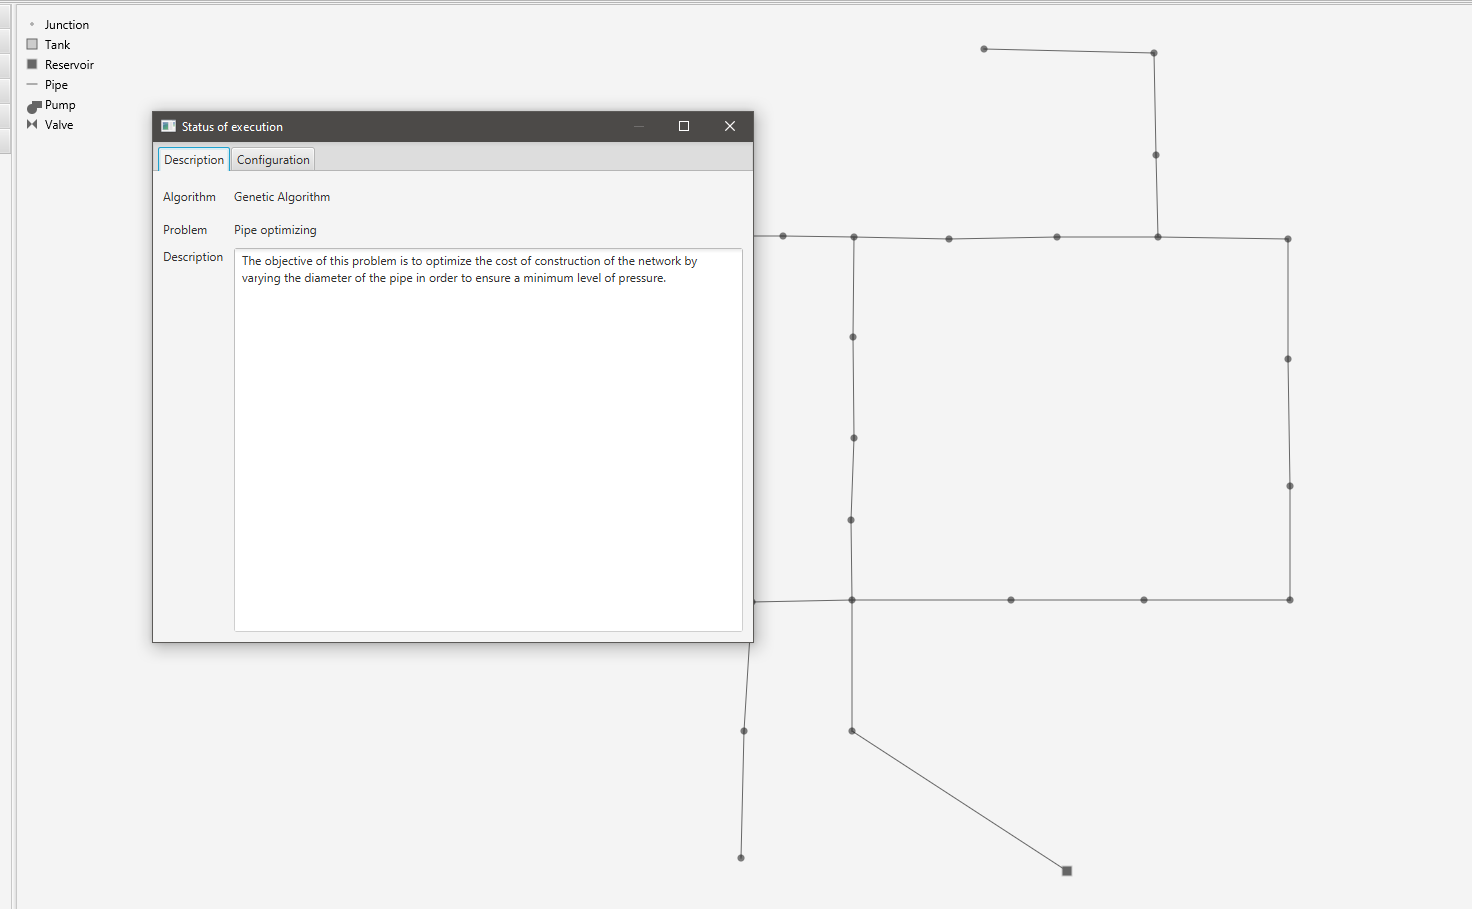
\includegraphics[width=\textwidth]{Capitulo4/assets/ConfiguracionProblema1.png}
	\caption{Ventana de descripci�n del problema.}
	\label{fig:ventana_descripcion}
\end{figure}

\begin{figure}[H]
  \centering
  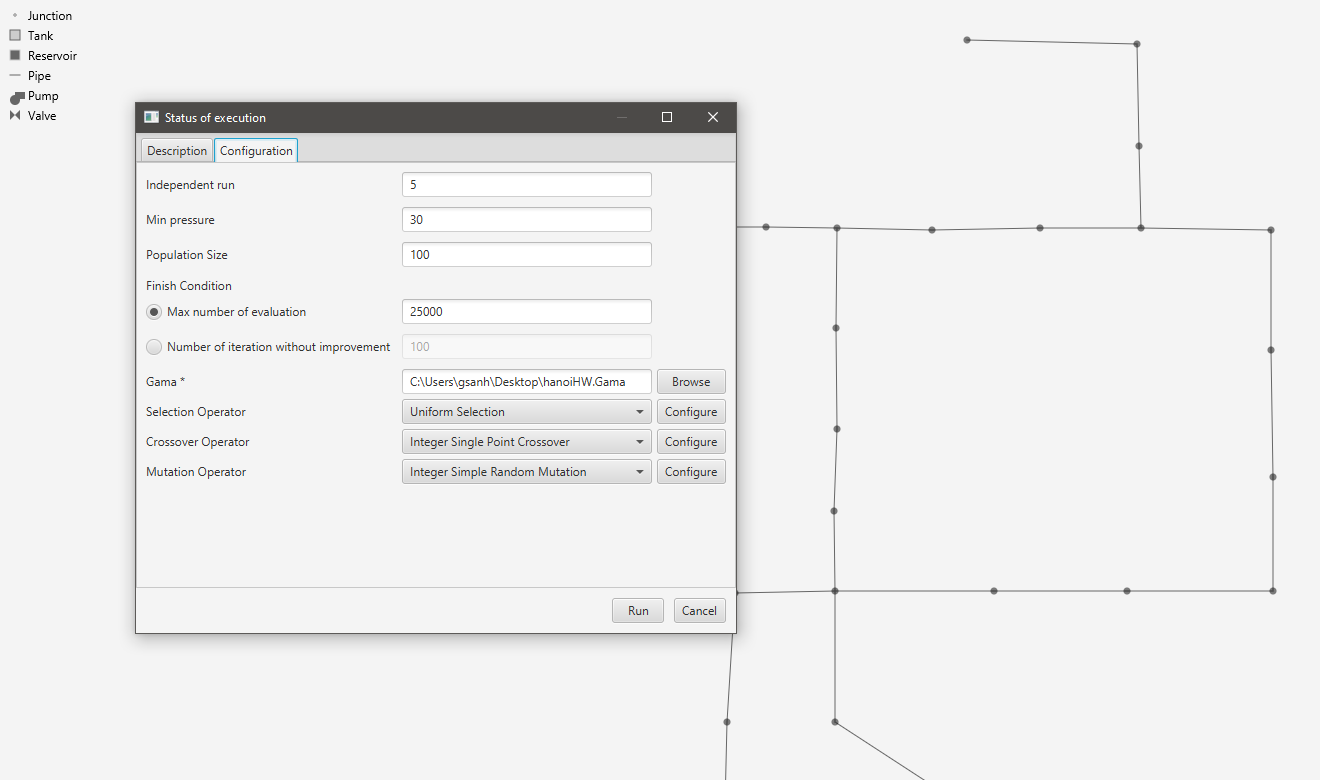
\includegraphics[width=\textwidth]{Capitulo4/assets/ConfiguracionProblema2.png}
	\caption{Ventana de configuraci�n del problema.}
	\label{fig:ventana_configuracion_problema}
\end{figure}

\begin{figure}[H]
  \centering
  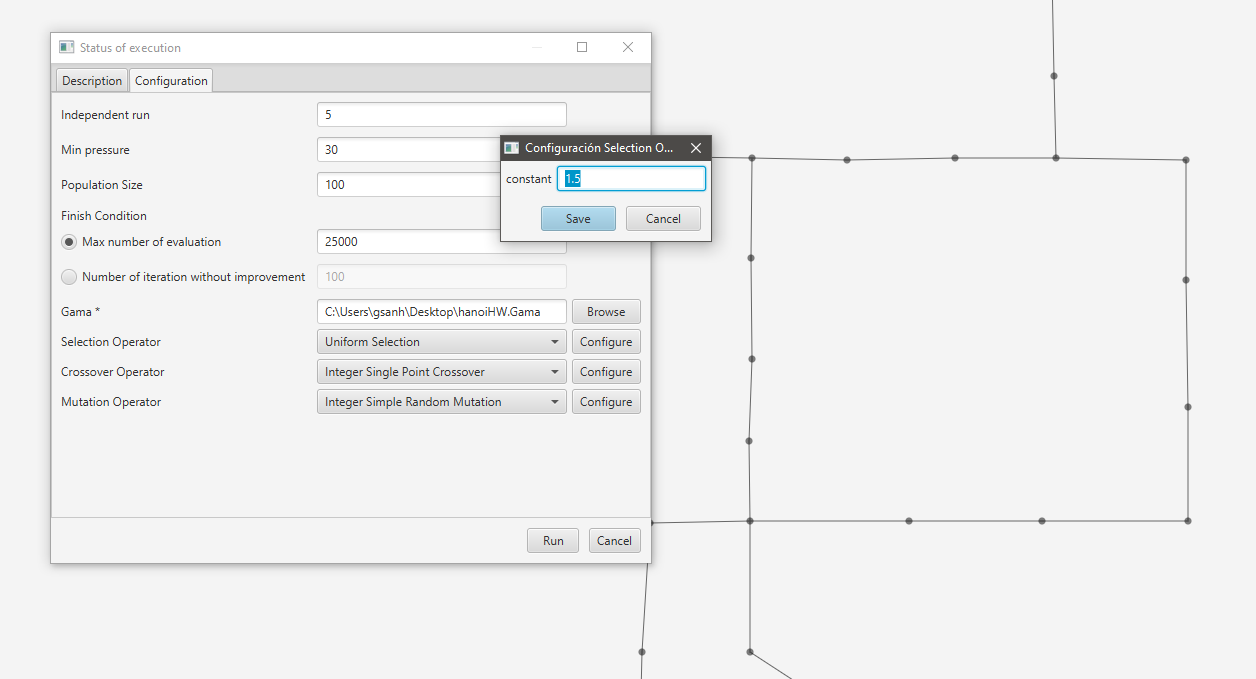
\includegraphics[width=\textwidth]{Capitulo4/assets/ConfiguracionProblema3.png}
	\caption{Ventana de configuraci�n de par�metros del operador \textit{UniformSelection}}
	\label{fig:ventana_operador}
\end{figure}

\begin{figure}[H]
  \centering
  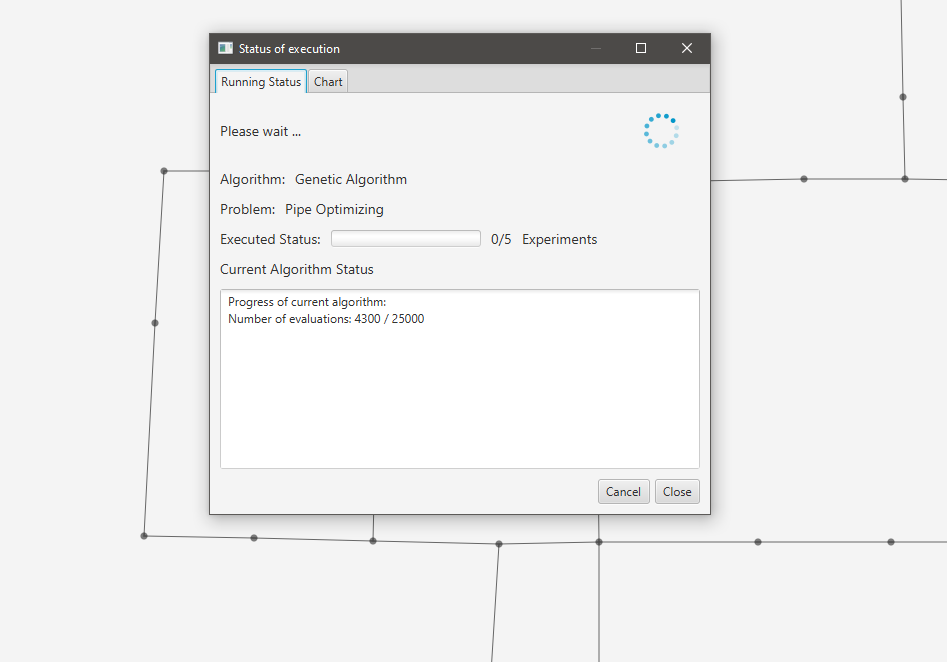
\includegraphics[width=\textwidth]{Capitulo4/assets/VentanaDeEjecucionMono.png}
	\caption{Ventana del retroalimentaci�n mostrada durante la ejecuci�n}
	\label{fig:ventana_retroalimentacion}
\end{figure}

\begin{figure}[H]
  \centering
  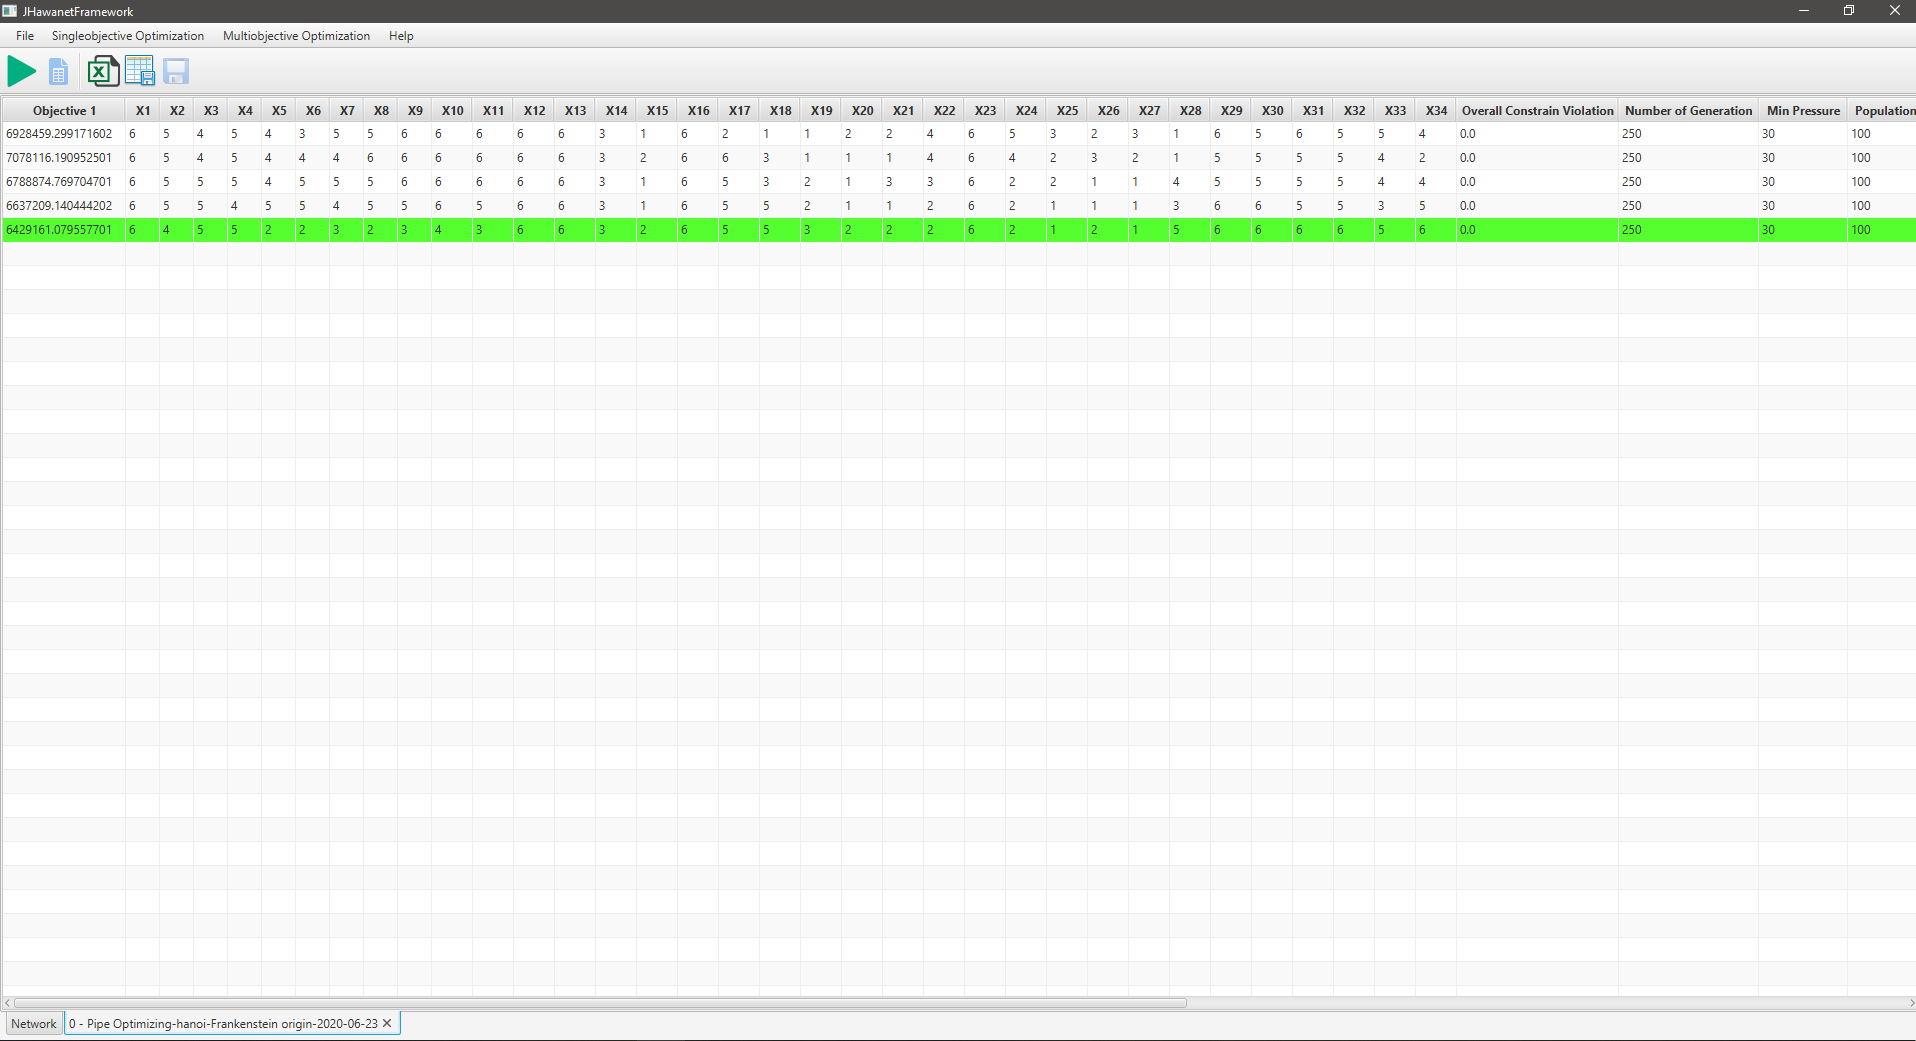
\includegraphics[width=\textwidth]{Capitulo4/assets/VentanaDeResultadosMono.png}
	\caption{Ventana de resultados generada cuando termina la ejecuci�n para el problema monoobjetivo Pipe Optimizing}
	\label{fig:ventana_resultados_opt}
\end{figure}

\paragraph{Funcionalidad 3}: La Figura~\ref{fig:ventana_simulacion_hyd} muestra la ventana con los resultados de una simulaci�n hidr�ulica para la red cargada.


\begin{figure}[H]
  \centering
  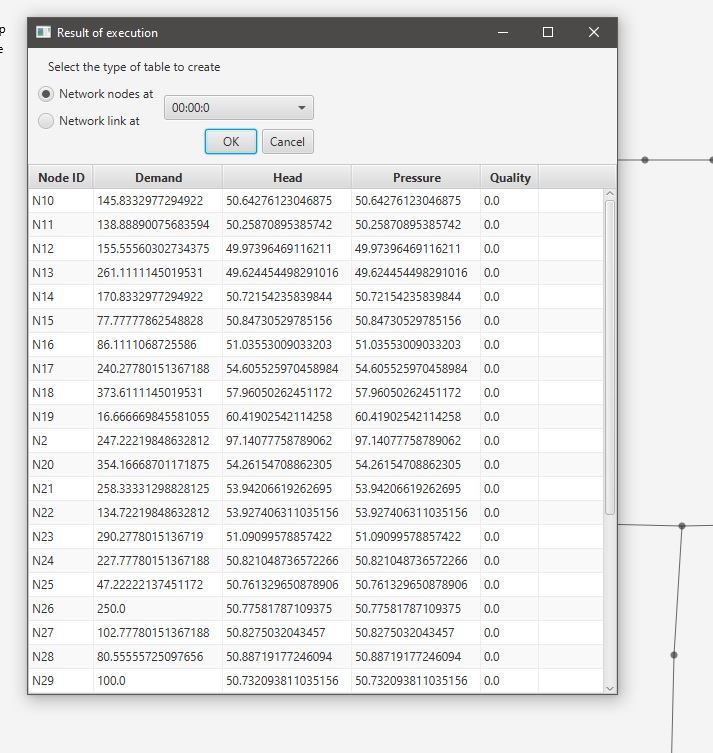
\includegraphics[width=\textwidth]{Capitulo4/assets/VentanaDeSimulacionHidraulica.png}
	\caption{Ventana de simulaci�n hidr�ulica utilizando los valores del archivo de red}
	\label{fig:ventana_simulacion_hyd}
\end{figure}

\subsection{Modelo matem�tico de los problemas}
En esta subsecci�n se presentan los modelos matem�ticos de los problemas resueltos, as� como la representaci�n de sus soluciones.

\subsubsection{\textit{Pipe Optimizing}}
\textit{Pipe Optimizing} es un problema de dise�o cuyo objetivo es minimizar el costo de inversi�n en la construcci�n de las tuber�as. Para �sto, se busca aquella combinaci�n de di�metros que disminuyan el costo de la construcci�n de las tuber�as a la vez que se cumplen las restricci�n de presi�n m�nima impuesta sobre la red. La ecuaci�n \ref{eq:costos_de_inversion} presentada en \cite{Pereyra2017} muestra la ecuaci�n a optimizar.
	
\begin{equation}
    \label{eq:costos_de_inversion}
    \begin{aligned}
        \text{Costo de inversi�n} = \sum_{i=1}^{N} (C_i \times D_i \times L_i)
    \end{aligned}
\end{equation}

En la ecuaci�n anteriormente presentada el termino $C_i$ se refiere al costo unitario de la tuber�a $i$, el t�rmino $D_i$ corresponde al di�metro de la tuber�a y finalmente $L_i$ hace referencia su longitud. Como se menciono anteriormente, el problema debe satisfacer la siguiente restricci�n:

\begin{equation}
    \label{eq:restriccion_costo_inversion}
    \begin{aligned}
        H_i < H_{min}
    \end{aligned}
\end{equation}

\noindent donde $H_i$ corresponde a la presi�n sobre la tuber�a $i$ y $H_{min}$ a la presi�n m�nima de la red.

La soluci�n retornada por el algoritmo utilizado, en este caso GA, se puede ver en la Figura~\ref{fig:solution_pipe_optimizing}. En dicha soluci�n los valores que toman la variable de decisi�n corresponden al �ndice a una tabla donde se encuentra el di�metro y el costo de la tuber�a. El largo de la tuber�a esta configurado en el archivo de configuraci�n de red (El archivo con extensi�n inp). 

\begin{figure}[H]
    \centering
    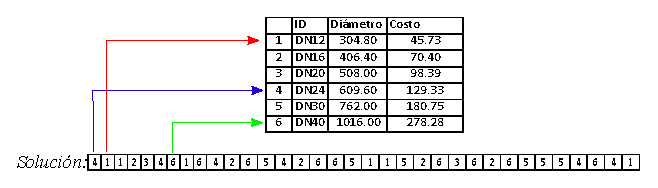
\includegraphics[width=\textwidth]{Capitulo4/assets/representacion_solucion_monoobjetivo.eps}
    \caption{Representaci�n de la soluci�n del problema monoobjetivo \textit{Pipe Optimizing}}
    \label{fig:solution_pipe_optimizing}
\end{figure}

\subsubsection{\textit{Pump Schedule}}

\textit{Pump Schedule} \cite{Makaremi2017, JHawanet-2019} es un problema de operaci�n que tiene como objetivos optimizar tanto el costo energ�tico, as� como el costo de operaci�n. A continuaci�n se expresan las ecuaciones utilizadas para calcular los objetivos y las restricciones.

Para el c�lculo de los costos energ�ticos se ocupa la siguiente ecuaci�n:
  
\begin{equation}
    \label{eq:costos_energeticos}
    \begin{aligned}
        C_E(S) &= \sum_{n=1}^{NP}\sum_{t=0}^{NT-1}(P_c(t) \times E_c(n, t) \times S(n, t))
    \end{aligned}
\end{equation}

\noindent donde:
\begin{itemize}
    \item	$C_E(S)$: Costos energ�tico.
    \item   $NP$: El numero de bombas.
    \item 	$NT$: N�mero de periodos de simulaci�n. El m�ximo son 24 horas.
    \item 	$P_c(t)$: La tarifa energ�tica en el periodo $t$.
    \item 	$E_c(n, t)$: Consumo energ�tico de la bomba $n$ en el tiempo $t$.
    \item 	$S(n,t)$: El estado de la bomba. 1 si esta encendida y 0 si esta apagada.
\end{itemize}

Para calcular el consumo energ�tico de la bomba $n$ se utiliza la siguiente formula:
\begin{equation}
    \label{eq:costos_energeticos}
    \begin{aligned}
        E_c(n, t) &= \frac{10^{-3} \times \gamma \times Q(n, t) \times h(n, t)}{e(n, t)}
    \end{aligned}
\end{equation}

\noindent donde:
\begin{itemize}
    \item	$\gamma$: Peso del agua.
    \item   $Q(n, t)$: Flujo a trav�s de la bomba $n$ en el tiempo $t$
    \item 	$h(n, t)$: Altura manom�trica de la bomba.
    \item 	$e(n, t)$: Eficiencia de la bomba $n$ en el tiempo $t$.
\end{itemize}

Para c�lcular el costo de bombeo se c�lcula el n�mero de encendido y apagados de todas las bombas en el periodo de tiempo analizado. Matem�ticamente la funci�n para calcular dicho costo corresponde a:

\begin{equation}
    \label{eq:costos_de_mantenimiento}
    \begin{aligned}
        C_N(S) &= \sum_{n=1}^{NP}\sum_{t=0}^{NT-1}r_t
    \end{aligned}
\end{equation}
donde:
\begin{itemize}
    \item $C_N(S)$ Costo de mantenimiento.
    \item $r_t$: Valor indicando si en el periodo $t$ hubo un cambio de estado en la bomba desde apagado a encendido. Este valor es 1 cuando la bomba ha sido encendida.
\end{itemize}

La funciones \ref{eq:costos_energeticos} y \ref{eq:costos_de_mantenimiento} deben cumplir las siguientes restricciones:
% restricciones asociadas a la conservaci�n de la masa y la energ�a; la presi�n m�nima, el caudal en la bomba $n$ y el nivel de agua almacenado en el reservorio en un periodo de tiempo especifico.

Conservaci�n de la masa:
\begin{equation}
    \label{eq:conservation_of_mass}
    \begin{aligned}
        \sum q_{in}-q_{out} &= C_j
    \end{aligned}
\end{equation}

\noindent donde:
\begin{itemize}
    \item $q_{in}$: Flujo de entrada.
    \item $q_{out}$: Flujo de salida.
    \item $C_j$: Consumo del nodo $j$.
\end{itemize}

Conservaci�n de la energ�a:
\begin{equation}
    \label{eq:conservation_of_energy}
    \begin{aligned}
        \sum h_f - \sum E_p &= 0
    \end{aligned}
\end{equation}

\noindent donde:
\begin{itemize}
    \item $h_f$: Perdida de energ�a por fricci�n.
    \item $E_p$: Energ�a aportada por la bomba.
\end{itemize}

Perdida de carga por fricci�n:
\begin{equation}
    \label{eq:pipe_head_losses}
    \begin{aligned}
        h_f &= \frac{10.67 \times L_q^{1.85}}{CH^{1.85} \times D^{4.87}}
    \end{aligned}
\end{equation}

\noindent donde:
\begin{itemize}
    \item $L_q$: Largo de la tuber�a.
    \item $CH$: Coeficiente de Hazen-Williams.
    \item $D$: Di�metro de la tuber�a.
\end{itemize}

Presi�n m�nima:
\begin{equation}
    \label{eq:min_pressure}
    \begin{aligned}
        H_i < H_{min}
    \end{aligned}
\end{equation}

\noindent donde:
\begin{itemize}
    \item $H_i$: Presi�n en el nodo $i$.
    \item $H_{min}$: Presi�n m�nima.
\end{itemize}

Caudal:
\begin{equation}
    \label{eq:min_pressure}
    \begin{aligned}
        Q_{i,t} \geq Q_i^{max}
    \end{aligned}
\end{equation}

\noindent donde:
\begin{itemize}
    \item $Q_{i,t}$: Caudal del nodo $i$ en el tiempo $t$.
    \item $Q_i^{max}$: Caudal m�ximo del nodo $i$.
\end{itemize}

Nivel de dep�sito:
\begin{equation}
    \label{eq:min_pressure}
    \begin{aligned}
        TS_{i, NT} \geq TS_{i, 0}
    \end{aligned}
\end{equation}

\noindent donde:
\begin{itemize}
    \item $TS_{i, NT}$: Nivel del reservorio $i$ en el tiempo $t$.
    \item $TS_{i, 0}$: Nivel del reservorio $i$ en el tiempo $0$.
\end{itemize}

En la Figura~\ref{fig:solution_pump_schedule} muestra como se codifica la soluci�n a este problema. Como se puede observar la soluci�n cuenta con 24 variables de decisi�n correspondiente a las 24 horas del d�a. Cada variable es un �ndice a la matriz de combinaciones posibles para cada bomba. Posteriormente, se genera una matriz binaria en donde cada fila es una bomba, cada columna es el periodo y el valor es el estado de la bomba en dicho periodo. Esta matriz binaria es usada para calcular el n�mero de cambios de estado en las bombas de la ecuaci�n \ref{eq:costos_de_mantenimiento}, asi como para obtener el estado de la bomba en el periodo $t$ de la ecuaci�n \ref{eq:costos_energeticos} referente al termino $S(n, t)$.

\begin{figure}[H]
    \centering
    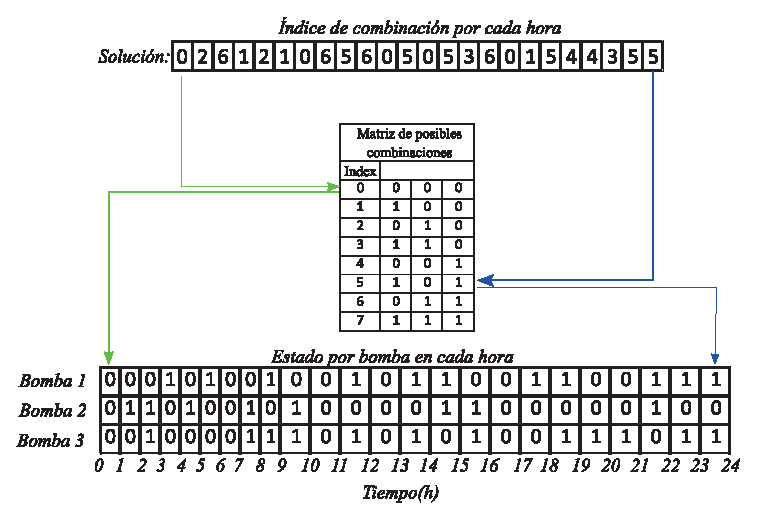
\includegraphics[width=\textwidth]{Capitulo4/assets/representacion_solucion_multiobjetivo.eps}
    \caption{Representaci�n de la soluci�n problema multiobjetivo \textit{Pump Schedule}}
    \label{fig:solution_pump_schedule}
  \end{figure}

\section{Pruebas}

En esta ultima fase del proceso de desarrollo se procede a evaluar las funcionalidades implementadas.

Para la evaluaci�n de las funcionalidades de la aplicaci�n se aplican una serie de casos de prueba. Estos casos de prueba se dividen en dos categor�a. Los casos de prueba utilizados para pruebas automatizadas y aquellos casos de prueba utilizados para pruebas manuales. 

Los casos de prueba automatizados son aquellos realizados utilizando herramientas que permiten automatizar las tareas necesarias para evaluar los elementos que componen el software. Estas pruebas se llevan a cabo sobre los elementos del software como las clases o funciones implementadas. Estos casos de prueba se identificaron usando diversos m�todos de testeo como herramienta para especificar los casos que deben ser evaluados. Los m�todos utilizados principalmente para identificar los casos de prueba fueron los de caja negra y los de caja blanca.

Los caso de prueba manuales se refieren a aquellas pruebas realizadas con la ayuda humana. Es decir, realizados personalmente por un ser humano. Estos casos de prueba son utilizados principalmente para comprobar la funcionalidades de la interfaz gr�fica donde automatizar las pruebas tiene una mayor complejidad.

% \begin{table}
%    \begin{center}
%        \caption{Actividades fase de pruebas}
%        \bigskip
%        \begin{tabular}{||c|c||}
%             \hline
%             N� Iteraci�n & Tareas\\ [0.5ex] 
%             \hline\hline
%             1 & \\
%             2 & \\
%             3 & \\
%             4 & \\
%             5 & \\
%             6 & \\
%             \hline
%        \end{tabular}
%        \label{fig:cambios_pruebas}
%    \end{center}
% \end{table}

A continuaci�n se presentan las pruebas realizadas que abarcan a cada una de las funcionalidades escogidas.

\paragraph{Funcionalidad 1}: El Cuadro~\ref{fig:MT001} muestra la especificaci�n formal para el caso de prueba manual realizado sobre esta funcionalidad.
\paragraph{Funcionalidad 2}: Los Cuadros~\ref{fig:MT002} y \ref{fig:MT003} muestran la especificaci�n para los casos de prueba manuales de esta funcionalidad.
\paragraph{Funcionalidad 3}: Los Cuadros~\ref{fig:MT013}, \ref{fig:MT014}, \ref{fig:MT015} y \ref{fig:MT016} muestran la especificaci�n para los casos de prueba manuales de esta funcionalidad.

\begin{prueba}[fig:MT001][Especificaci�n caso de prueba manual MT001][0.8\textwidth]
    \TestID{MT001}
    \Titulo{Visualizaci�n de la red.}
    \Caracteristica{Mostrar visualizaci�n de la red.}
    \Objetivo{Confirmar que la red puede ser leida desde un archivo ``.inp'' y ser visualizada en la applicaci�n.}
    \Configuracion{El equipo tiene la applicaci�n JHawanetFramework lista para ejecutar.}
    \DatosPrueba{%
        inp: hanoi-Frankenstein.inp
    }
    \AccionesPrueba{%
        1. Abrir JHawanetFramework\\
        2. Cargar archivo de red.
    }
    \ResultadosEsperados{El sistema muestra la red leida desde un archivo inp gr�ficamente en la applicaci�n.}
\end{prueba}

\begin{prueba}[fig:MT002][Especificaci�n caso de prueba manual MT002][0.8\textwidth]
    \TestID{MT002}
    \Titulo{Optimizaci�n monoobjetivo realizada completamente.}
    \Caracteristica{Realizar simulaci�n monoobjetivo.}
    \Objetivo{Confirmar que se puede llevar a cabo la resoluci�n del problema \textit{PipeOptimizing} sobre la red abierta.}
    \Configuracion{El equipo tiene la applicaci�n JHawanetFramework lista para ejecutar.}
    \DatosPrueba{%
        independentRun = 10\\
        Archivo inp: hanoi-Frankenstein.inp\\
        Archivo gama: hanoiHW.Gama
    }
    \AccionesPrueba{%
        1. Abrir JHawanetFramework\\
        2. Cargar archivo de red.\\
        3. Seleccionar el problema \textit{PipeOptimizing del men�}.\\
        4. Configurar el problema usando la ventana de configuraci�n.\\
        5. Realizar la optimizaci�n.
    }
    \ResultadosEsperados{Al terminar la optimizaci�n el sistema muestra una interfaz con las soluciones generadas por la optimizaci�n. Debe haber tantas soluciones como el numero de configuraciones independientes (\textit{independentRun}).}
\end{prueba}

\begin{prueba}[fig:MT003][Especificaci�n caso de prueba manual MT003][0.8\textwidth]
    \TestID{MT003}
    \Titulo{Optimizaci�n monoobjetivo cancelada.}
    \Caracteristica{Realizar simulaci�n monoobjetivo.}
    \Objetivo{Confirmar que se puede llevar a cabo la resoluci�n del problema \textit{PipeOptimizing} sobre la red abierta y que se puede cancelar el proceso  cerrando la ventana o pulsando cancelar.}
    \Configuracion{El equipo tiene la applicaci�n JHawanetFramework lista para ejecutar.}
    \DatosPrueba{%
        Archivo inp: hanoi-Frankenstein.inp\\
        Archivo gama: hanoiHW.Gama
    }
    \AccionesPrueba{%
        1. Abrir JHawanetFramework\\
        2. Cargar archivo de red.\\
        3. Seleccionar el problema \textit{PipeOptimizing del men�}.\\
        4. Configurar el problema usando la ventana de configuraci�n.\\
        5. Realizar la optimizaci�n.
    }
    \ResultadosEsperados{Al cancelar la busqueda de soluciones la ventana de estado indica que la optimizaci�n a sido detenida.}
\end{prueba}

\begin{prueba}[fig:MT013][Especificaci�n caso de prueba manual MT013][0.8\textwidth]
    \TestID{MT013}
    \Titulo{Simulaci�n hidr�ulica sobre red de un solo tiempo.}
    \Caracteristica{Realizar simulaci�n con configuraci�n de archivo de red.}
    \Objetivo{Confirmar que se puede realizar la simulaci�n utilizando los valores del archivo de red.}
    \Configuracion{El equipo tiene la applicaci�n JHawanetFramework lista para ejecutar.}
    \DatosPrueba{%
        Archivo inp: hanoi-Frankenstein.inp\\
        Archivo gama: hanoiHW.Gama
    }
    \AccionesPrueba{%
        1. Abrir JHawanetFramework\\
        2. Cargar archivo de red.\\
        3. Pulsar bot�n \textit{Execute} de la ventana principal.
    }
    \ResultadosEsperados{
        Ejecuci�n realizada sin ningun error.
    }
\end{prueba}

\begin{prueba}[fig:MT014][Especificaci�n caso de prueba manual MT014][0.8\textwidth]
    \TestID{MT014}
    \Titulo{Ver resultados de la simulaci�n hidr�ulica de un solo tiempo}
    \Caracteristica{Realizar simulaci�n con configuraci�n de archivo de red.}
    \Objetivo{Confirmar que se puede visualizar los resultados de la simulaci�n realizada.}
    \Configuracion{El equipo tiene la applicaci�n JHawanetFramework lista para ejecutar.}
    \DatosPrueba{%
        Archivo inp: hanoi-Frankenstein.inp\\
        Archivo gama: hanoiHW.Gama
    }
    \AccionesPrueba{%
        1. Abrir JHawanetFramework\\
        2. Cargar archivo de red.\\
        3. Pulsar bot�n \textit{Execute} de la ventana principal.\\
        4. Pulsar bot�n \textit{Results} de la ventana principal.
    }
    \ResultadosEsperados{
        Una interfaz que permite seleccionar si se quieren ver los resultados para los enlaces o los nodos.
    }
\end{prueba}

\begin{prueba}[fig:MT015][Especificaci�n caso de prueba manual MT015][0.8\textwidth]
    \TestID{MT015}
    \Titulo{Simulaci�n hidr�ulica sobre red de mas de un tiempo.}
    \Caracteristica{Realizar simulaci�n con configuraci�n de archivo de red.}
    \Objetivo{Confirmar que se puede realizar la simulaci�n utilizando los valores del archivo de red.}
    \Configuracion{El equipo tiene la applicaci�n JHawanetFramework lista para ejecutar.}
    \DatosPrueba{%
        Archivo inp: Vanzyl.inp\\
        Archivo gama: VanzylConfiguration.json
    }
    \AccionesPrueba{%
        1. Abrir JHawanetFramework\\
        2. Cargar archivo de red.\\
        3. Pulsar boton \textit{Execute} de la ventana principal.
    }
    \ResultadosEsperados{
        Ejecuci�n realizada sin ningun error.
    }
\end{prueba}

\begin{prueba}[fig:MT016][Especificaci�n caso de prueba manual MT016][0.8\textwidth]
    \TestID{MT016}
    \Titulo{Ver resultados de la simulaci�n hidr�ulica de mas de un tiempo}
    \Caracteristica{Realizar simulaci�n con configuraci�n de archivo de red.}
    \Objetivo{Confirmar que se puede visualizar los resultados de la simulaci�n realizada.}
    \Configuracion{El equipo tiene la applicaci�n JHawanetFramework lista para ejecutar.}
     \DatosPrueba{%
        Archivo inp: Vanzyl.inp\\
        Archivo gama: VanzylConfiguration.json
    }
    \AccionesPrueba{%
        1. Abrir JHawanetFramework\\
        2. Cargar archivo de red.\\
        3. Pulsar bot�n \textit{Execute} de la ventana principal.\\
        4. Pulsar bot�n \textit{Results} de la ventana principal.
    }
    \ResultadosEsperados{
        Una interfaz que permite seleccionar si se quieren ver los resultados para los enlaces o los nodos. Adicionalmente, permite escoger el tiempo de simulaci�n y listar los resultados para todos los tiempos de un elemento de la red espec�fico.
    }
\end{prueba}

La especificaci�n de las restantes pruebas realizadas se encuentra en el \textbf{Anexo~\ref{appendix:prueba}}.
\chapter{Metodolog�a de evaluaci�n}
\chapter{Evaluaci�n de la soluci�n}

En este cap�tulo se da a conocer la metodolog�a de evaluaci�n y su aplicaci�n, detallando las fases y los resultados de �stas, con el fin de evaluar la soluci�n implementada.


\section{Metodolog�a de evaluaci�n}

La metodolog�a que se ha escogido para realizar este an�lisis consiste en el estudio de caso. Para llevar a cabo este estudio de caso se comienza realizando el dise�o del caso de estudio, luego se realiza la recolecci�n de datos, el an�lisis de los datos recolectados y finalmente de reportan los resultados junto con las conclusiones del estudio.

En el dise�o del caso, se define el caso a estudiar, los objetivos, el protocolo para conducir el estudio, las caracter�sticas que se quieren evaluar y los sujetos de prueba o unidad de an�lisis.

En la recolecci�n de datos, se aplica el instrumento a la unidad de an�lisis.

Durante la etapa de an�lisis, se procesan los datos presentando una serie de gr�ficas que ayudar�n a visualizar de mejor manera la informaci�n recolectada.

Finalmente, durante la etapa de reporte se presentar�n las conclusiones de la aplicaci�n del caso de estudio.

\section{Dise�o del estudio de caso}

En esta secci�n, como se menciono anteriormente, se detalla el plan de acci�n previo a la aplicaci�n del caso.

\subsection{Elecci�n del caso}

El caso a evaluar consiste en el software desarrollado durante este proyecto de titulaci�n. Como ya se sabe, es un software que permite buscar soluciones a problemas hidr�ulicos utilizando algoritmos metaheur�sticos.

\subsection{Objetivos de la investigaci�n}

El estudio que se quiere llevar a cabo es un estudio del tipo cualitativo, transversal y descriptivo, con el cual se busca comprender como el sistema desarrollado se desempe�a en la practica y su grado de aceptaci�n.

Como pregunta de investigaci�n se establece la siguiente:

\begin{center}
    \textit{�C�mo el sistema desarrollado trabaja en la pr�ctica?}
\end{center}

\subsection{Caracter�sticas a evaluar}
\label{cap:caracteristicas_a_evaluar}

Las caracter�sticas que se buscan evaluar mediante la aplicaci�n del caso de estudio son las siguientes:

\begin{itemize}
    \item \textbf{Funcionalidad}: Con esta caracter�stica se busca evaluar lo que la aplicaci�n puede hacer, es decir, si el sistema cumple con las operaciones que se busca realizar con el programa.
    \item \textbf{Facilidad de uso}: Esta caracter�stica busca medir la usabilidad del software, es decir, que tan f�cil es de usar la aplicaci�n. 
    \item \textbf{Utilidad}: Con este criterio se busca medir el valor de la aplicaci�n. Con valor, nos referimos a si las funcionalidades implementadas por el sistema son de utilidad para quien haga uso de soluci�n.
    \item \textbf{Utilidad del manual de usuario}: Con este criterio se busca evaluar el manual de usuario realizado y si este fue de ayuda para aprender y poder conocer la aplicaci�n.
\end{itemize}

 La medici�n de cada una de estas caracter�sticas se lleva a cabo usando encuestas.

\subsection{Protocolo para conducir el estudio de caso}
El objetivo de este protocolo es establecer una gu�a para realizar la recolecci�n de datos.

Debido a la complejidad de coordinar y agendar una reuni�n se opt� por realizar la recolecci�n de datos de manera as�ncrona.

El protocolo para llevar a cabo la evaluaci�n del sistema consiste en:

\begin{enumerate}
    \item Enviar la aplicaci�n junto con su manual a los participantes del estudio.
    \item Dar un tiempo para que el participante del estudio se interiorice con la aplicaci�n.
    \item Enviar la encuesta a los participantes.
\end{enumerate}

El instrumento utilizado para evaluar la soluci�n se encuentra en el \textbf{Anexo~\ref{appendix:evaluacion}}.

\subsection{Unidad de an�lisis}
La recopilaci�n de datos se lleva a cabo sobre profesionales con conocimientos tanto en el �rea computacional, hidr�ulica y metaheur�sticas. 

\section{Consideraciones preliminar}

\textbf{Consideraciones t�cnicas}:
En esta secci�n se mencionan algunas consideraciones preliminares t�cnicas como de usuario.
\begin{itemize}
    \item Para utilizar el software se requiere el sistema operativo Window con la versi�n de Java 1.8.
    \item Para crear una nueva red se debe usar un programa externo. Este programa es Epanet y la red debe ser exportada a un archivo .inp. Debido a que la versi�n en espa�ol y la en ingl�s de Epanet crean el archivo .inp cambiando algunas palabras claves que forman parte del archivo de configuraci�n de red exportado, se opt� por utilizar el formato de la versi�n en ingl�s de Epanet dentro del programa desarrollado.
    \item Para visualizar los resultados de la exportaci�n a un documento de Excel, se requiere dicho programa o alguna alternativa que permita visualizar las hojas de c�lculo con extensi�n .xslx.
\end{itemize}

\textbf{Consideraciones para los usuarios}:
\begin{itemize}
    \item Para poder implementar nuevos problemas y algoritmos se requiere tener conocimientos en hidr�ulica y programaci�n, as� como tambi�n en metaheur�sticas. Si no se requiere implementar nuevos elementos, los conocimientos en programaci�n no son tan necesarios, mientras que los de metaheur�sticas e hidr�ulica s�, con el objetivo de saber como interpretar los resultados.
\end{itemize}

\section{Recolecci�n de datos}
En esta secci�n se presentan los participantes del estudio y se detallan las caracter�sticas del instrumento utilizado para la obtenci�n de datos.

\subsubsection{Participantes}
Los participantes del proceso de recolecci�n de datos fueron los siguientes:

\bigskip
\textbf{Evaluador}
\begin{itemize}
    \item Gabriel Sanhueza
\end{itemize}

\textbf{Usuario}

\begin{itemize}
    \item Yamisleydi Salgueiro
    \item Marco Alsina
    \item Sergio Silva
\end{itemize}

\subsubsection{Instrumentos para la recolecci�n de los datos}

Para el proceso de recolecci�n de los datos se utilizaran encuestas. La encuesta esta dise�ada para evaluar las caracter�sticas mencionadas en la subsecci�n~\ref{cap:caracteristicas_a_evaluar}. La funcionalidad y la utilidad se eval�an usando la escala de Likert. En cuanto a la usabilidad, este se eval�a usando la escala de usabilidad de SUS.

La escala de usabilidad de SUS cuenta con 10 preguntas, las cuales a efecto de la presente evaluaci�n son:

\begin{enumerate}
    \item Creo que usar�a esta aplicaci�n frecuentemente.
    \item Encuentro esta aplicaci�n innecesariamente complejo.
    \item Creo que la aplicaci�n fue f�cil de usar.
    \item Creo que necesitar�a ayuda de una persona con conocimientos t�cnicos para usar esta aplicaci�n.
    \item Las funciones de esta aplicaci�n est�n bien integradas.
    \item Creo que la aplicaci�n es muy inconsistente.
    \item Imagino que la mayor�a de la gente aprender�a a usar esta aplicaci�n en forma muy r�pida.
    \item Encuentro que la aplicaci�n es muy dif�cil de usar.
    \item Me siento confiado al usar esta aplicaci�n.
    \item Necesit� aprender muchas cosas antes de ser capaz de usar esta aplicaci�n.
\end{enumerate}

La encuesta aplicada se encuentra en el \textbf{Anexo~\ref{appendix:evaluacion}}.

\section{An�lisis de datos}
En esta secci�n se presenta el an�lisis de los datos. El an�lisis se realiza de manera independiente por cada una de las caracter�sticas a evaluar, en donde se muestran los resultados utilizando herramientas como gr�ficos y tablas. Adicionalmente, se provee una interpretaci�n de los resultados.

A continuaci�n se presentan los resultados por cada categor�a evaluada.

\subsection{Funcionalidad}

En la Figura \ref{fig:app_functionality} se presentan los resultados de la evaluaci�n de la funcionalidad en forma de un gr�fico de barras. Mientras, que en el Cuadro \ref{fig:app_functionality_table} se muestra la tabla con el porcentaje obtenido por cada alternativa de la evaluaci�n.

\begin{figure}[H]
    \centering
    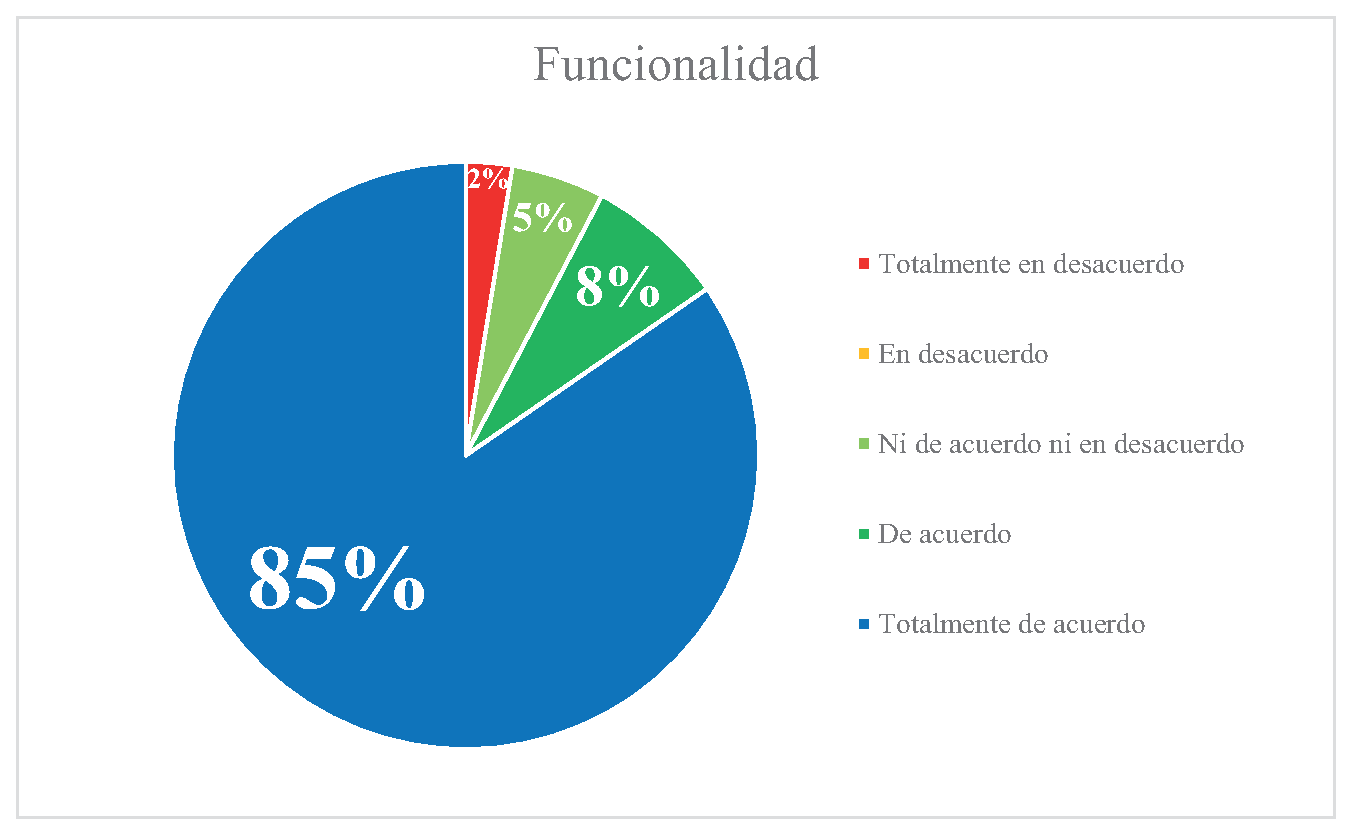
\includegraphics[width=\textwidth]{Capitulo5/assets/funcionality.eps}
    \caption{Gr�fico circular de los resultados de la evaluaci�n de funcionalidad de la aplicaci�n}
    \label{fig:app_functionality}
\end{figure}

\begin{table}[H]
    \centering
    \caption{Resultados de la evaluaci�n de la funcionalidad}
    \bigskip
    \begin{tabular}{||c|c||}
        \hline
        Respuesta & Porcentaje Obtenido\\ [0.5ex] 
        \hline\hline
        Totalmente en desacuerdo & 2.6\%\\
        \hline
        En desacuerdo & 0.0\%\\
        \hline
        Ni de acuerdo ni en desacuerdo & 5.1\%\\
        \hline
        De acuerdo & 7.7\%\\
        \hline
        Totalmente de acuerdo & 84.6\%\\
        \hline
        Total & 100\%\\
        \hline
    \end{tabular}
    \label{fig:app_functionality_table}
\end{table}

Como se puede ver en la Figura \ref{fig:app_functionality} y en el Cuadro \ref{fig:app_functionality_table}, el 93\% de las respuestas est�n ``de acuerdo'' y ``totalmente de acuerdo'' con el hecho de que las funcionalidades que incorpora la aplicaci�n han sido implementadas correctamente. Por otro lado, el 5\% de las respuestas apuntan a que no se est� ``ni de acuerdo ni en desacuerdo'' con el hecho de si las funcionalidades est�n correctamente integradas. Mientras que el 2\% de las respuestas apuntan a que las funcionalidades no fueron integradas correctamente o que hab�a una carencia de alguna de ellas.

\subsection{Usabilidad}
El Cuadro \ref{fig:sus} presenta la escala de clasificaci�n utilizada para comparar el puntaje SUS.

\begin{table}[H]
    \centering
    \caption{Escala de rangos de \textit{SUS Score}~\cite{sus-scale}}
    \bigskip
    \begin{tabular}{||c|c||}
        \hline
        \textit{SUS Score} & Calificaci�n\\ [0.5ex] 
        \hline\hline
        $>$ 80,3 & Excelente\\
        \hline
        68 - 80,3 & Buena\\
        \hline
        68 & Regular\\
        \hline
        51 - 68 & Mala\\
        \hline
        $<$ 51 & Terrible\\
        \hline
    \end{tabular}
    \label{fig:sus}
\end{table}

La aplicaci�n del instrumento de medici�n dio como resultado un promedio:

$$ \bar{x}_{SUS} = 79.17$$

con una desviaci�n est�ndar de :

$$ s_{SUS} = 9.46$$

De esto se puede concluir que en el aspecto de usabilidad la aplicaci�n se le califica como "Buena".

\subsection{Utilidad}
La Figura \ref{fig:app_utility} y el Cuadro \ref{fig:app_utility_table} muestran los resultados obtenidos de la evaluaci�n de la utilidad de la aplicaci�n.

\begin{figure}[H]
    \centering
    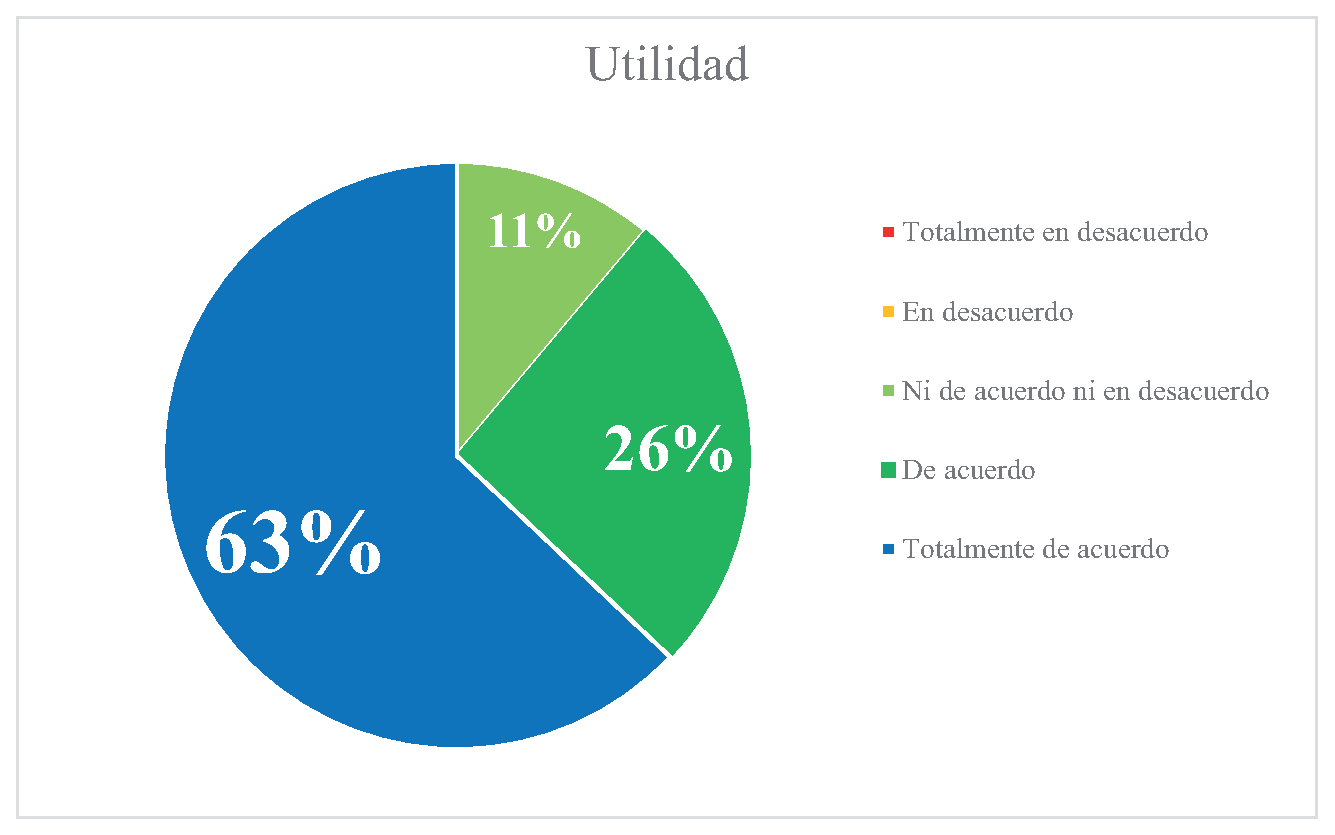
\includegraphics[width=\textwidth]{Capitulo5/assets/utility.eps}
    \caption{Gr�fico circular de los resultados de la evaluaci�n de utilidad de la aplicaci�n}
    \label{fig:app_utility}
\end{figure}

\begin{table}[H]
    \centering
    \caption{Resultados de la evaluaci�n de la utilidad}
    \bigskip
    \begin{tabular}{||c|c||}
        \hline
        Respuesta & Porcentaje Obtenido\\ [0.5ex] 
        \hline\hline
        Totalmente en desacuerdo & 0.0\%\\
        \hline
        En desacuerdo & 0.0\%\\
        \hline
        Ni de acuerdo ni en desacuerdo & 11.1\%\\
        \hline
        De acuerdo & 25.9\%\\
        \hline
        Totalmente de acuerdo & 63.0\%\\
        \hline
        Total & 100\%\\
        \hline
    \end{tabular}
    \label{fig:app_utility_table}
\end{table}

De la Figura \ref{fig:app_utility} y Cuadro \ref{fig:app_utility_table} se observa que el 89\% de las respuestas indican que se est� ``totalmente de acuerdo'' o ``de acuerdo'' con que las funcionalidades implementadas en la aplicaci�n son de utilidad para los encuestados. Mientras que un 11\% indican que no se est� ``ni se acuerdo ni en desacuerdo'' con si realmente son �tiles o no.

\subsection{Utilidad del manual de usuario}
Los resultados de la evaluaci�n de la utilidad del manual de usuario se presentan en la Figura \ref{fig:manual_utility} y el Cuadro \ref{fig:app_manual_utility_table}.

\begin{figure}[H]
    \centering
    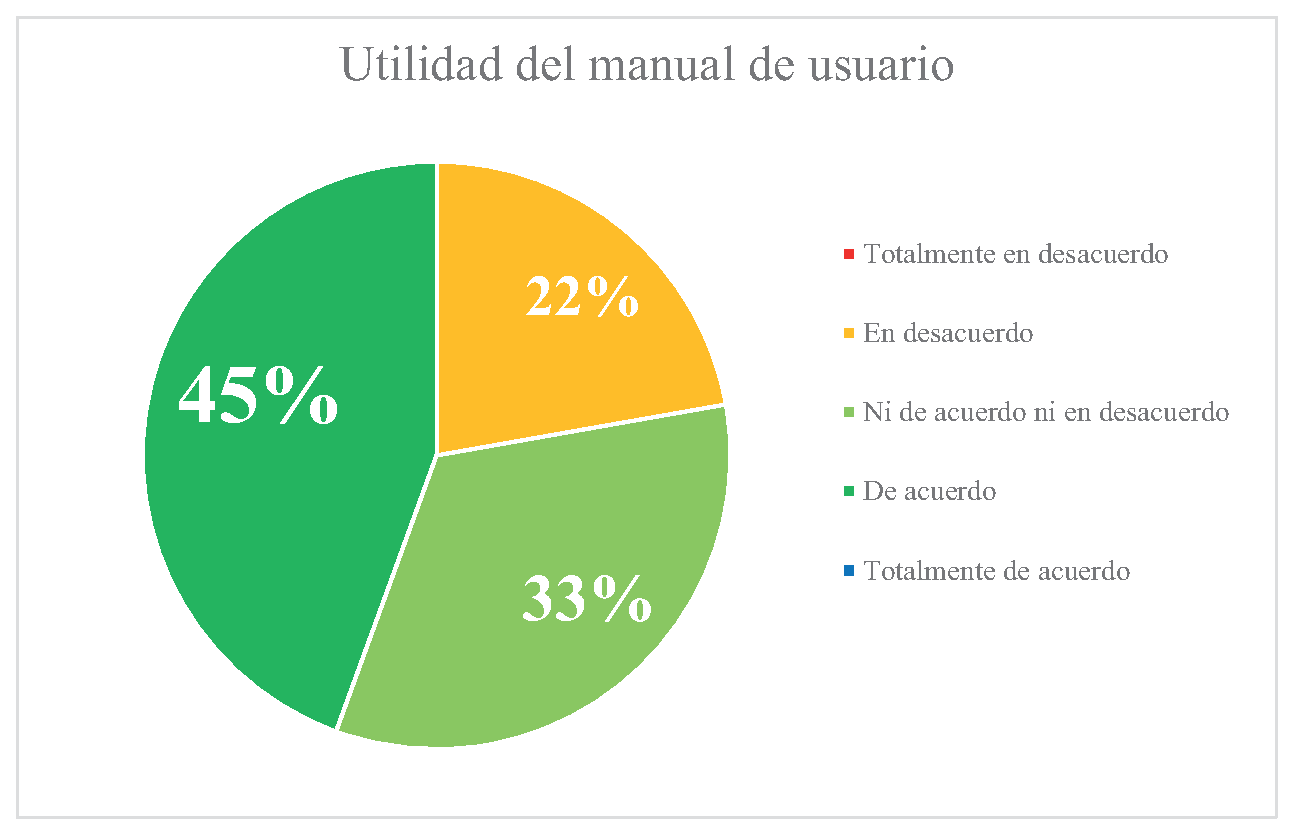
\includegraphics[width=\textwidth]{Capitulo5/assets/manual_utility.eps}
    \caption{Gr�fico circular de los resultados de la evaluaci�n de la utilidad del manual de usuario}
    \label{fig:manual_utility}
\end{figure}

\begin{table}[H]
    \centering
    \caption{Resultados de la evaluaci�n de la utilidad del manual de usuario}
    \bigskip
    \begin{tabular}{||c|c||}
        \hline
        Respuesta & Porcentaje Obtenido\\ [0.5ex] 
        \hline\hline
        Totalmente en desacuerdo & 0.0\%\\
        \hline
        En desacuerdo & 22.2\%\\
        \hline
        Ni de acuerdo ni en desacuerdo & 33.3\%\\
        \hline
        De acuerdo & 44.4\%\\
        \hline
        Totalmente de acuerdo & 0.0\%\\
        \hline
        Total & 100\%\\
        \hline
    \end{tabular}
    \label{fig:app_manual_utility_table}
\end{table}

Con respecto a la utilidad del manual de usuario, de acuerdo a los resultados presentados en la Figura \ref{fig:manual_utility} y el Cuadro \ref{fig:app_manual_utility_table}, se puede apreciar que el 45\% de las respuestas apuntan a que se est� ``de acuerdo'' con que el manual de usuario presentado junto con el software fue de utilidad para comprender como utilizarlo y realizar ciertas tareas con �ste. Por otro lado, un 33\% indica que no se est� ``ni de acuerdo ni en desacuerdo'' con si el manual de usuario fue �til o no, mientras que el 22\% indica que se est� en ``desacuerdo'' con la utilidad del manual y por lo tanto que es deficiente y debiera ser mejorado.

\section{Conclusiones del estudio}
Durante esta secci�n se presentan las conclusiones obtenidas a partir de la aplicaci�n del caso de estudio.

A partir de los resultados obtenidos se puede concluir que la aplicaci�n cumple con los criterios de funcionalidad, usabilidad y utilidad. Por lo tanto, puede ser ocupada en un contexto real y ser ocupada para buscar soluciones a problemas de RDA.

Por otra parte, si bien el manual de usuario sirvi� para utilizar y comprender la aplicaci�n este debe ser mejorado incorporando m�s detalles y ejemplos de las funcionalidades explicadas.
\clearpage

\chapter{Conclusiones Y Trabajos Futuros}
En este cap�tulo se presentan las conclusiones del trabajo desarrollado asi como la propuestas de trabajo futuro que puede ser realizados sobre la herramienta.

\section{Conclusiones}
Se ha desarrollado un software que permite optimizar los procesos de dise�o y operaci�n en redes de agua potable. Dicho software, incorpora por defecto dos problemas y dos algoritmos. Los problemas implementados son el de dise�o de RDA basado en la selecci�n del di�metro de tuber�as y el problema del r�gimen de bombeo. En cuanto a los algoritmos a�adidos, se encuentran el Algoritmo Gen�tico y el algoritmo NSGAII. 

Los objetivos definidos para este trabajo son exitosamente logrados en el tiempo planificado. 

La aplicaci�n de la metodolog�a se llevo a cabo realizando las cuatro fases correspondientes a requisitos, dise�o, implementaci�n y pruebas en cada una de las iteraciones. Al finalizar el periodo de desarrollo todas las funcionalidades solicitadas se encuentran implementadas.

La metodolog�a de desarrollo utilizada fue la adecuada dando como resultado documentaci�n extra que puede ser consultada por aquellos que deseen continuar mejorando el sistema en futuros trabajos. Los documentos generados son la especificaci�n de requisitos (Anexo~\ref{appendix:requisito}), la especificaci�n del dise�o (Anexo~\ref{appendix:diseno}); el manual de usuario (Anexo~\ref{appendix:manual}); y la especificaci�n de los casos de prueba (Anexo~\ref{appendix:prueba}). 

Gracias a la utilizaci�n de los patrones de Inversi�n de Control y Inyecci�n de Dependencias, as� como la utilizaci�n de las funcionalidades de Java, \textit{Java Reflection} y \textit{Java Annotation}, se logra mejorar la capacidad de extensibilidad del programa facilitando la incorporaci�n de nuevos algoritmos y problemas.

En relaci�n a la evaluaci�n de la soluci�n se concluye que la aplicaci�n incorpora las funcionalidades solicitadas en un principio por los interesados, el software es evaluado como ``bueno'' en cuanto a la usabilidad de acuerdo a la escala SUS utilizada y es de utilidad para los usuarios que se desempe�an en el �rea de redes de agua potable. Sin embargo, el manual de usuario debe ser mejorado incorporando m�s detalles de la aplicaci�n.

La aplicaci�n de encuentra disponible en el repositorio de GitHub \url{https://github.com/EinherjarSt/ProyectoDeMemoria}.

\section{Trabajo futuro}
Una vez terminado el desarrollo del proyecto se identifico por parte del desarrollador, los colaboradores y los sujetos del estudio realizado, una serie de cadencias y detalles que pueden ser mejorados, as� como algunas funcionalidades extras que incrementan el valor de la aplicaci�n. �stas se listan a continuaci�n:

\begin{itemize}
    \item Agregar nuevos algoritmos, operadores y problemas al sistema.
    \item Recortar el n�mero de decimales con que se presentan los resultados en la aplicaci�n.
    \item Exportar el gr�fico de la red como una imagen vectorial.
    \item Exportar el gr�fico de soluciones para uno y dos objetivos como una imagen vectorial.
    \item Cambiar el tama�o de los iconos de la red cuando se posicione el cursor sobre �stos.
    \item Permitir agregar formulas utilizando Latex en la descripci�n de los algoritmos.
    \item Permitir utilizar distintos algoritmos en un mismo experimento.
    \item Incorporar m�tricas de comparaci�n entre algoritmos.
    \item Mostrar en la interfaz los patrones de demanda y bombeo de la red cuanto �sta los especifique.
    \item Permitir restablecer los valores por defecto en la pesta�a de configuraci�n del problema.
    \item Incorporar una cola de trabajo para ejecutar m�s de una optimizaci�n a la vez.
\end{itemize}

%% ambiente glosario
\begin{glosario}
  \item[RDA] Este es el significado del primer t�rmino, realmente no se bien lo que significa pero podr�a haberlo averiguado si hubiese tenido un poco mas de tiempo.
  \item[GA] Este si se lo que significa pero me da lata escribirlo...
\end{glosario}


%% genera las referencias
\bibliography{refs}


%% comienzo de la parte de anexos
\appendixpart

%% contenido del primer anexo
\appendix{Documento de especificaci�n de requisitos}



%% contenido del segundo anexo
\appendix{Documento de dise�o}

%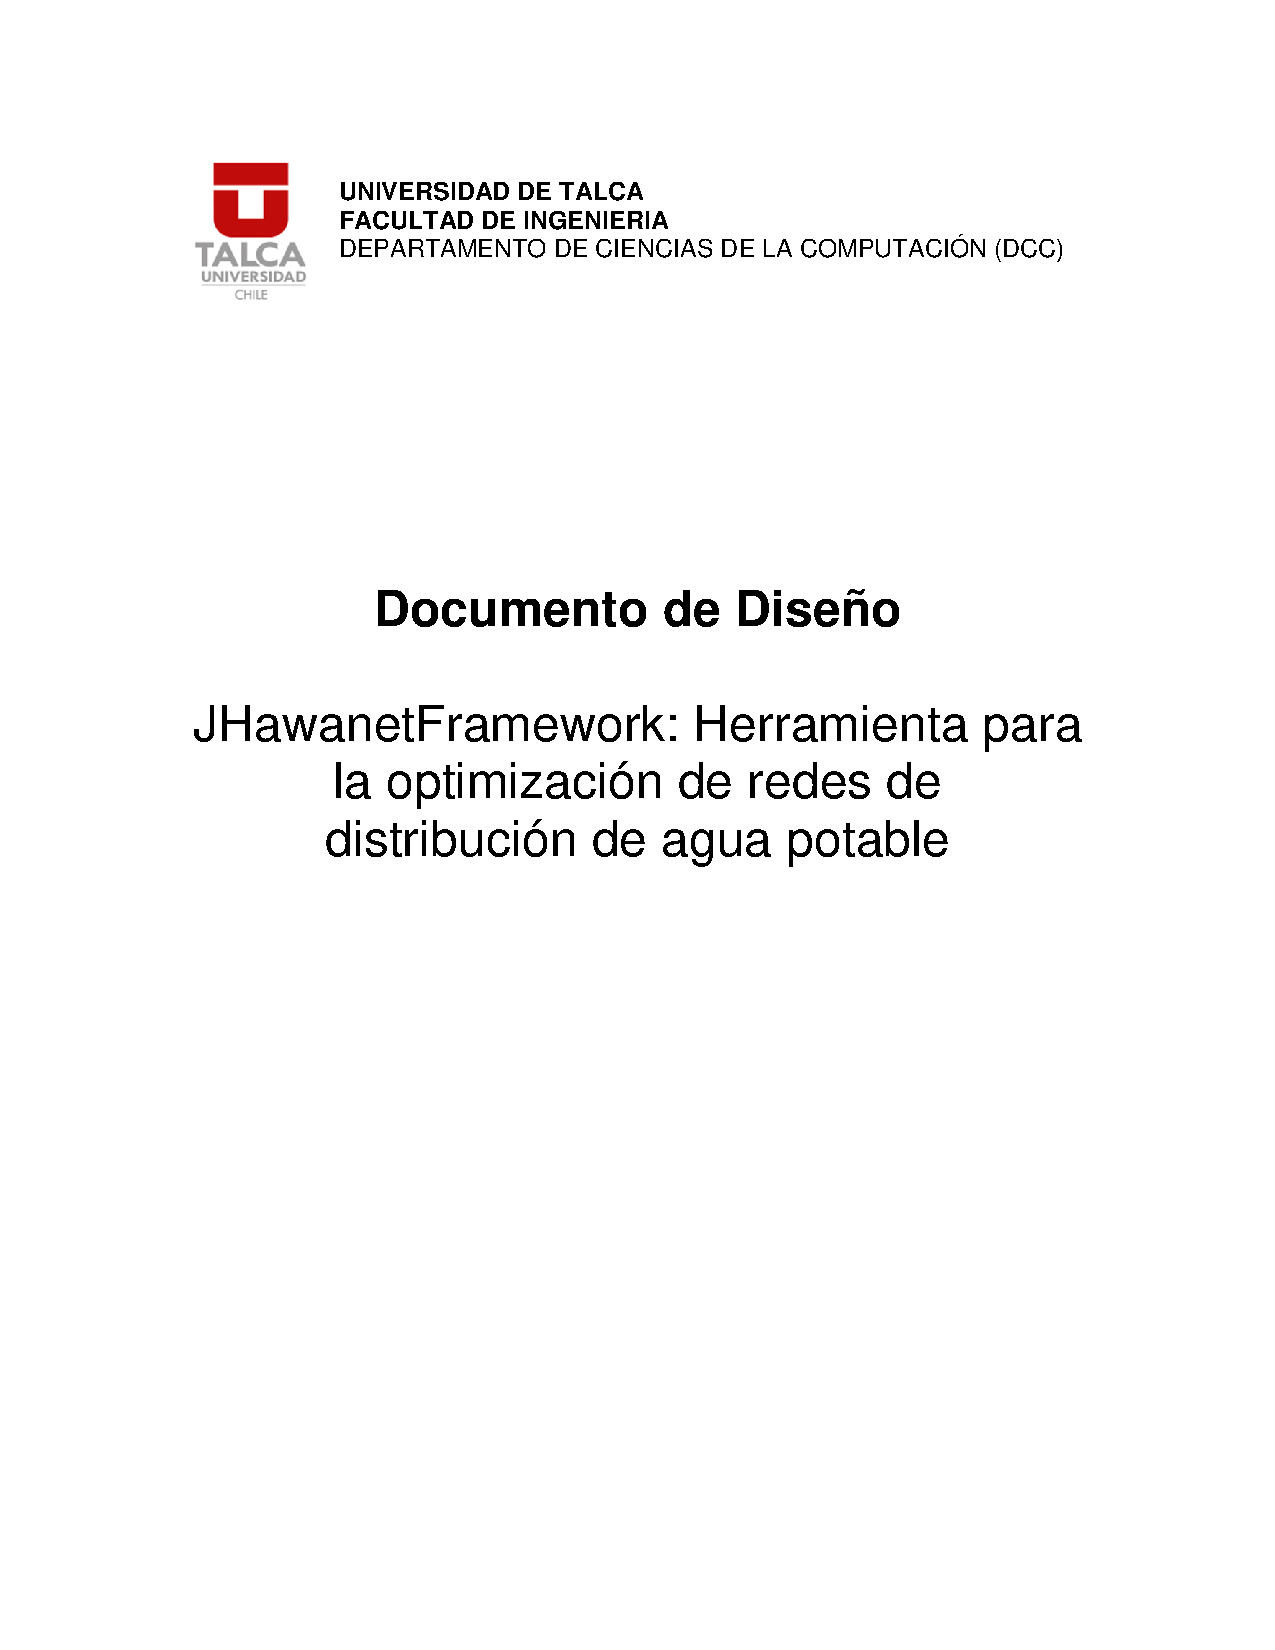
\includepdf[pages=-]{Documentodedisenio.pdf}
\appendix{Manual de usuario}

\appendix{Documento de casos de prueba}

\appendix{Cuestionario para la evaluaci�n de la aplicaci�n}
%% fin
\end{document}

   

